%\documentclass{article}

\documentclass[review,onefignum,onetabnum]{siamart190516}

%Packages
\usepackage[utf8]{inputenc}
\usepackage{geometry, graphicx,wrapfig}
\usepackage{enumerate}
%\usepackage{amsmath,amssymb,amsfonts,amsthm, bm}
\usepackage{amsmath,amssymb,amsfonts,bm}
\usepackage{xcolor} %just for visible comments.
\usepackage[linesnumbered,ruled,vlined,algo2e]{algorithm2e}
\usepackage[toc,page]{appendix}
\usepackage{makecell}
\usepackage{cleveref}

% New theorems and commands
%\newtheorem{theorem}{Theorem}[section]
%\newtheorem{lemma}[theorem]{Lemma}
%\newtheorem{corollary}[theorem]{Corollary}
\newtheorem{assump}[theorem]{Assumption}
\newcommand\mycommfont[1]{\ttfamily\textcolor{orange}{#1}}
%\SetCommentSty{mycommfont}
\newcommand{\R}{\mathbb{R}}
\newcommand{\F}{\mathbb{F}}
\newcommand{\dd}{\delta}
\newcommand{\tth}{\theta}
\newcommand{\bb}[1]{\mathbf{#1}}
\newcommand{\fl}{\mathrm{fl}}
\newcommand{\cO}{\mathcal{O}}

\newcommand\blfootnote[1]{%
	\begingroup
	\renewcommand\thefootnote{}\footnote{#1}%
	\addtocounter{footnote}{-1}%
	\endgroup
}

\crefname{algocf}{alg.}{algs.}
\Crefname{algocf}{Algorithm}{Algorithms}
%\theoremstyle{definition}
%\newtheorem{definition}{Definition}[section]
% Document
\title{Rounding error analysis of mixed-precision Householder QR algorithms}
\author{L. Minah Yang, Alyson Fox, and Geoffrey Sanders}
\date{\today}
\begin{document}

\maketitle
\begin{abstract}
	Although mixed precision arithmetic has recently garnered interest for training dense neural networks, many other applications could benefit from the  speed-ups and lower storage if applied appropriately. 
	The growing interest in employing mixed precision computations motivates the need for rounding error analysis that properly handles behavior from mixed precision arithmetic.
	We present a framework for mixed precision analysis that builds on the foundations of rounding error analysis presented in \cite{Higham2002} and demonstrate its practicality by applying the analysis to various Householder QR Algorithms. 
	%In addition, we present successful results from using mixed precision QR factorization for some small-scale benchmark problems in graph clustering. 
	\blfootnote{This work was performed under the auspices of the U.S. Department of Energy by Lawrence Livermore National Laboratory under Contract DE-AC52-07NA27344 and was supported by the LLNL-LDRD Program under Project No. 17-SI-004, LLNL-JRNL-795525-DRAFT.}
\end{abstract}
%TODO: remove graph stuff.
\section{Introduction}\label{sec:intro}
%The accuracy of a numerical algorithm depends on several factors, including numerical stability and well-conditionedness of the problem, both of which may be sensitive to rounding errors, the difference between exact and finite-precision arithmetic. 
%Low precision floats use fewer bits than high precision floats to represent the real numbers and naturally incur larger rounding errors. 
%Therefore, error attributed to round-off may have a larger influence over the total error when using low precision, and some standard algorithms may yield insufficient accuracy when using low precision storage and arithmetic.
%%TODO: MINAH comment reviewer 
%%that are in wide use may no longer be numerically stable when using half precision floating arithmetic and storage. 
%However, many applications exist that would benefit from the use of lower precision arithmetic and storage that are less sensitive to floating-point round off error, such as clustering or ranking graph algorithms \cite{vonLuxburg2007} or training dense neural networks \cite{micikevicius2018mixed}, to name a few.\par
%
%Many computing applications today require solutions quickly and often under low size, weight, and power constraints (low SWaP), e.g., sensor formation, etc. 
%%TODO: Reviewer #2 asks what does weight mean here.
%Computing in low-precision arithmetic offers the ability to solve many problems with improvement in all four parameters.
%Utilizing mixed precision, one can achieve similar quality of computation as high-precision and still achieve 
%speed, size, weight, and power constraint improvements. 
%There have been several recent demonstrations of computing using half-precision arithmetic (16 bits) achieving around half an order to an 
%order of magnitude improvement of these categories in comparison to double precision (64 bits).
%Trivially, the size and weight of memory required for a specific problem is 4$\times$.
%Additionally, there exist demonstrations that the power consumption improvement is similar
%\cite{fagan2016powerwall}.
%Modern accelerators (e.g., GPUs, Knights Landing, or Xeon Phi) are able to achieve this factor or better speedup improvements.
%Several examples include:
%(i)   2-4$\times$ speedup in solving dense large linear equations \cite{haidar2018iterative,haidar2019tensorcore},
%(ii)  12$\times$ speedup in training dense neural networks,
%and
%(iii) 1.2-10$\times$ speedup in small batched dense matrix multiplication \cite{abdelfattah2019batched} (up to 26$\times$ for batches of tiny matrices).
%Training deep artificial neural networks by employing lower precision arithmetic to various tasks such as multiplication \cite{Courbariaux2014Mult} and storage \cite{Courbariaux2014Storage} can easily be implemented on GPUs and are already a common practice in data science applications.\par
%
%The low precision computing environments that we consider are \emph{mixed precision} settings, which are designed to imitate those of new GPUs that employ multiple precision types for certain tasks. 
%For example, Tesla V100's TensorCores perform matrix products of half precision input data with exact products and single precision (32 bits) summation accumulate \cite{nvdia}.
%The existing rounding error analyses are built within what we call a \emph{uniform precision} setting, which is the assumption that all arithmetic operations and storage are performed via the same precision.
%In this work, we develop a framework for deterministic mixed precision rounding error analysis, and explore half-precision Householder QR factorization (HQR) algorithms for data and graph analysis applications. 
%QR factorization is known to provide a backward stable solution to the linear least squares problem and thus, is ideal for mixed precision. 
%%TODO: Remove it and just explain in response to reviewers. didn't serve purpose of paper mixed precision is an active area of research
%%TODO: algorithms with better stability should be looked at first in mixed precision. 
%
%However, additional analysis is needed as the additional round-off error will effect orthogonality, and thus the accuracy of the solution. 
%Here, we focus on analyzing specific algorithms in a specific set of types (IEEE754 half (fp16), single (fp32), and double(fp64)), but the framework we develop 
%could be used on different algorithms or different floating point types (such as bfloat16 in \cite{tagliavini2018floating}).\par
%
%This work discusses several aspects of using mixed precision arithmetic: (i) error analysis that can more accurately describe mixed precision arithmetic than existing analyses, (ii) algorithmic design that is more resistant against lower numerical stability associated with lower precision types, and (iii) an example where mixed precision implementation performs as sufficiently as double-precision implementations. 
%Our key findings are that the new mixed precision error analysis produces tighter error bounds, that some block QR algorithms by Demmel et al. \cite{Demmel2012} are able to operate in low precision more robustly than non-block techniques, and that some small-scale benchmark graph clustering problems can be successfully solved with mixed precision arithmetic.
%%TODO: MINAH rewrite outline of paper paragraph, and remove graph references in above paragraph.
%%In Section~\ref{sec:FPREA}, we will give an overview of the modern developments in hardware that motivates rounding error analysis that supports multiple precision types, and we will present a set of error analysis tools. 
%%The HQR factorization algorithm and a mixed precision rounding error analysis of its implementation is discussed in Section~\ref{sec:HQRf}.
%%In Section~\ref{sec:TSQR}, we present the TSQR algorithm as well as numerical experiments that show that TSQR can be useful in low precision environments. Section~\ref{sec:Apps} explores the use of low and mixed precision QR algorithms as subroutines for an application: spectral clustering.
\section{Background: Build up to rounding error analysis for inner products}\label{sec:background}
In this section, we introduce the basic motivations and tools for mixed-precision rounding error analysis needed for the {\it QR factorization}.
A matrix $\bb{A} \in \R^{m \times n}$ for $m\geq n$ can be written as
$$\bb{A} = \bb{QR},
\qquad
\bb{Q} \in \R^{m \times m},
\qquad
\bb{R} \in \R^{m \times n},$$
where $\bb{Q}$ is orthogonal, $\bb{Q}^\top \bb{Q} = \bb{I}_{m\times m}$ , and $\bb{R}$ is upper trapezoidal.
The above formulation is a \emph{full} QR factorization, whereas a more efficient \emph{thin} QR factorization results in $\bb{Q}_{1}\in\R^{m\times n}$ and $\bb{R}_{1}\in\R^{n\times n}$, that is
\[
\bb{A} = \bb{QR} = \begin{bmatrix}\bb{Q}_{1} & \bb{Q}_2\end{bmatrix} \begin{bmatrix}\bb{R}_{1} \\ \bb{0}_{m-n \times n}\end{bmatrix} = \bb{Q}_{1}\bb{R}_{1}.
\]
If $\bb{A}$ is full rank then the columns of $\bb{Q}_{1}$ are orthonormal (i.e. $\bb{Q}_{1}^{\top}\bb{Q}_{1}=\bb{I}_{n\times n}$) and $\bb{R}_1$ is upper triangular.
In many applications, computing the \emph{thin} decomposition requires less computation and is sufficient in performance. 
While important definitions are stated explicitly in the text, Table~\ref{table:notation} serves to establish basic notation.
\begin{table}[H]
	\centering
	%\begin{tabular}{|m{3cm}|m{9cm}|c|}
	\begin{tabular}{|m{1.7cm}|m{10.3cm}|c|}
		\hline
		%DONE: change table have the following 3 columns, add sections
		Symbol(s) & Definition(s) & Section(s) \\ \hline
		${\bb x}$, ${\bb A}$  & Vector, matrix  & \ref{sec:background} \\
		%	${\bb A}$ & Matrix & \ref{sec:intro}\\
		%$m$, $n$ & Number of rows, columns of matrix, or length of vector&  \ref{sec:intro}\\
		%$i$, $j$ & Row, column index of matrix or vector & \ref{sec:HQRfA} \\
		%$\|{\bf x}\|_2$, $\|\bb{A}\|_2$ & Vector operator 2-norm & \ref{sec:HQRf}\\
		%$|c|$, $|\bb{x}|$ ,$|\bb{A}|$ & Absolute value of constant, all elements of vector, matrix & \ref{sec:HQRf} \\
		%$\bb{x}_i$, $\hat{e}_i$  & $i^{th}$ element of vector $\bb{x}$, cardinal vector &  \ref{sec:HQRfA}, \ref{sec:HQRf}\\
		%$\bb{A}[a:b, c:d]$ &Rows $a$ to $b$ and columns $c$ to $d$ of matrix $\bb{A}$ & \ref{sec:HQRfA}\\
		%$\bb{A}[a:b,:]$, $\bb{A}[:,c:d]$ & Rows $a$ to $b$, columns $c$ to $d$ of matrix $\bb{A}$& \ref{sec:HQRfA}\\
		\hline
		$\bb{Q}$  & Orthogonal factor $\bb{A}\in\R^{m\times n}$: $m$-by-$m$ (full) or $m$-by-$n$ (thin)  & \ref{sec:background}\\
		$\bb{R}$ & Upper triangular or trapezoidal factor of $\bb{A}\in\R^{m\times n}$:  $m$-by-$n$ (full) or $n$-by-$n$ (thin)  &  \ref{sec:background}\\ 
		%$\bb{A}^{(k)}$ & Matrix $\bb{A}$ after $k$ Householder transformations. &\ref{sec:HQRfA}\\
		\hline
		$\fl(\bb{x})$, $\hat{\bb{x}}$ & Quantity $\bb{x}$ calculated from floating point operations & \ref{sec:backgroundRE} \\
		$b$, $t$, $\mu$, $\eta$  & Base/precision/mantissa/exponent bits & \ref{sec:backgroundRE} \\
		%\tt{Inf} & Values outside the range of representable numbers & \ref{sssec:NormalizeHV} \\ %https://www.doc.ic.ac.uk/~eedwards/compsys/float/nan.html
		$k$ & Number of successive FLOPs &  \ref{sec:backgroundRE}\\
		$u^q$ & Unit round-off for precision $t_q$ and base $b_q$: $\frac{1}{2}b_q^{1-t_q}$ & \ref{sec:backgroundRE} \\ 
		$\dd^{q}$ &Quantity bounded by: $|\dd^{q}| < u^q$ &  \ref{sec:backgroundRE} \\
		$\gamma^{q}_{k}$,  $\tth^{q}_{k}$& $\frac{ku^q}{1-ku^q}$, Quantity bounded by: $|\tth^{q}_{k}|\leq\gamma^q_{k}$ &  \ref{sec:backgroundRE} \\
		%$\tth_{q}^{(k)}$ & Quantity bounded by: $|\tth_{q}^{(k)}|\leq\gamma_q^{(k)}$ &  \ref{sec:FPREA} \\ 
		\hline
			%$\bb{0}_{m\times n}$, $\bb{I}_{n}$ & $m$-by-$n$ zero matrix, $n$-by-$n$ identity  matrix &  \ref{sec:intro}\\
		%$\bb{I}_{n} & $n$-by-$n$ identity  matrix  & \ref{sec:HQRfA} \\
		%$\bb{I}_{m\times n}$ & $[\bb{I}_{n} \quad \bb{0}_{n \times (m-n)}]^{\top}$ & \ref{sec:TSQR}\\ \hline
		%$\bb{P}_{\bb{v}}$, $\bb{P}_i$ & Householder transformation define by $\bb{v}$, $i^{th}$ Householder transformation in HQR& \ref{sec:HQRfA}\\
		%$\bb{P}_i$ & $i^{th}$ Householder transformation in the HQR algorithm & \ref{sec:HQRfA} \\ 
		\hline		
		%$u^h, u^l, u_w$ & Unit round-off for sum, product, and storage (write) & \ref{ssec:IP}\\ 
		%		$\gamma_{p,q}^{(k_l,k_q)}$ & $(1+\gamma_p^{(k_l)})(1+\gamma_q^{(k_q)})-1$ & \ref{ssec:IP}\\
		%		$\tth_{p,q}^{(k_l,k_q)}$ & Quantity bounded by: $|\tth_{p,q}^{(k_l,k_q)}|<\gamma_{p,q}^{(k_l,k_q)}$ & \ref{ssec:IP}\\
		\hline
	\end{tabular}
	\caption{Basic definitions}
	\label{table:notation}
\end{table}
\Cref{sec:backgroundRE} introduces basic concepts for rounding error analysis, and \Cref{sec:backgroundIP} exemplifies the need for mixed-precision rounding error analysis using the inner product.
\subsection{Basic rounding error analysis of floating point operations}\label{sec:backgroundRE}
We use and analyze the IEEE 754 Standard floating point number systems.
Let $\F \subset \R$ denote the space of some floating point number system with base $b\in\mathbb{N}$, precision $t\in\mathbb{N}$, significand $\mu\in\mathbb{N}$, and exponent range $[\eta_{\text{min}}, \eta_{\text{max}}]\subset \mathbb{Z}$.
Then every element $y$ in $\F$ can be written as 
\begin{equation}
y = \pm \mu\times b^{\eta-t},
\label{eqn:FPbasic}
\end{equation} 
where $\mu$ is any integer in $[0,b^{t}-1]$ and $\eta$ is an integer in  $[\eta_{\text{min}}, \eta_{\text{max}}]$.
While base, precision, and exponent range are fixed and define a floating point number,the sign, significand, and exponent identifies a unique number within that system.
Although operations we use on $\R$ cannot be replicated exactly due to the finite cardinality of $\F$, we can still approximate the accuracy of analogous floating point operations (FLOPs).
We adopt the rounding error analysis tools described in \cite{Higham2002}, which allow a relatively simple framework for formulating error bounds for complex linear algebra operations. 
A short analysis of FLOPs (see Theorem 2.2 \cite{Higham2002}) shows that the relative error is 
controlled by the unit round-off, $u:=\frac{1}{2}b^{1-t}$. \par 
\vspace{.2cm}
\begin{table}[H]
	\begin{tabular}{||l|c|c|c|c|c|c||} 
		\hline 
		Name & $b$ & $t$ & \# of exponent bits & $\eta_{\text{min}}$ & $\eta_{\text{max}}$ & unit round-off $u$ \\ \hline 
		fp16 (IEEE754 half)& 2 & 11 & 5 & -15 & 16  & {\tt 4.883e-04} \\ \hline 
		fp32 (IEEE754 single)& 2 & 24 & 8 & -127 & 128  & {\tt 5.960e-08} \\ \hline 
		fp64 (IEEE754 double)& 2 & 53 & 11 & -1023 & 1024 & {\tt 1.110e-16} \\ \hline 
	\end{tabular}
%\end{center}
	\caption{IEEE754 formats and their primary attributes.} % with $j$ exponent bits ranging from $1-2^{j-1}$ to $2^{j-1}$.}
	\label{table:ieee}
\end{table}
\vspace{.2cm}

Let `op' be any basic operation from the set OP $=\{+, -, \times, \div\}$ and let $x,y\in \R$.
The true value $(x\text{ op }y)$ lies in $\R$, and it is rounded using some conversion to a floating point number, $\fl(x\text{ op }y)$, admitting a rounding error. 
The IEEE 754 Standard requires \emph{correct rounding}, which rounds the exact solution $(x\text{ op }y)$ to the closest floating point number and, in case of a tie, to the floating point number that has a mantissa ending in an even number.
\emph{Correct rounding} gives us an assumption for the error model where a single basic floating point operation yields a relative error, $\dd$, bounded in the following sense:
\begin{equation}
\fl(x\text{ op }y) = (1 + \dd)(x\text{ op }y),\quad |\dd|\leq u, \quad \text{op}\in\{+, -, \times, \div\}. \label{eqn:singlefpe}
\end{equation}
We use \cref{eqn:singlefpe} as a building block in accumulating errors from successive FLOPs.
For example, consider computing $x+y+z$, where $x,y,z\in\R$ with a machine that can only compute one operation at a time.
Then, there is a rounding error in computing $\hat{s_1}:= \fl(x+y) = (1+\dd)(x+y)$, and another rounding error in computing $\hat{s_2}:= \fl(\hat{s_1}+ z) = (1+\tilde{\dd})(\hat{s_1}+z)$, where $|\dd|,|\tilde{\dd}|<u$.
Then, 
\begin{equation}
\fl(x+y+z) = (1+\tilde{\dd})(1+\dd) (x+y) + (1+\tilde{\dd}) z.\label{eqn:FPbasic3}
\end{equation}
Multiple successive operations introduce multiple rounding error terms, and keeping track of all errors is challenging.
Lemma \ref{lem:gamma} introduces a convenient and elegant bound that simplifies accumulation of rounding error. 
\begin{lemma}[Lemma 3.1 \cite{Higham2002}]
	\label{lem:gamma}
	Let $|\dd_i|<u$ and $\rho_i \in\{-1, +1\}$, for $i = 1 , \cdots, k$ and $ku < 1$. Then, 
	\begin{equation}
	\prod_{i=1}^k (1+\dd_i)^{\rho_i} = 1 + \tth_{k},
	\qquad \mbox{where} \qquad
	|\tth_{k}|\leq \frac{ku}{1-ku}=:\gamma_{k}.
	\end{equation}
	We also use 
	\begin{equation*}
	\tilde{\gamma}_{k} = \frac{cku}{1-cku},
	\end{equation*}
	where $c>0$ is a small integer.  
\end{lemma}
In other words, $\tth_{k}$ represents the accumulation of rounding errors from $k$ successive operations, and it is bounded by $\gamma_{k}$. 
Allowing $\tth_{k}$'s to be any arbitrary value within the corresponding $\gamma_{k}$ bounds further aids in keeping a clear, simple error analysis. 
Applying this lemma to our example of adding three numbers results in
\begin{equation}
\fl(x+y+z) = (1+\tilde{\dd})(1+\dd) (x+y) + (1+\tilde{\dd})z = (1+\tth_{2})(x+y) + (1+\tth_{1})z. \label{eqn:FPbasic4}
\end{equation}
Since $|\tth_{1}| \leq \gamma_{1} < \gamma_{2}$, we can further simplify \cref{eqn:FPbasic4} to
\begin{equation}
\fl(x+y+z) = (1+\tilde{\tth}_{2})(x+y+z), \quad \mbox{where} \quad |\tilde{\tth}_{2}| \leq \gamma_{2}, \label{eqn:FBbasic5}
\end{equation}
at the cost of a slightly larger upper bound. 
Typically, error bounds formed in the fashion of \cref{eqn:FBbasic5} are converted to relative errors in order to put the error magnitudes in perspective.
The relative error bound for our example is
\begin{equation*}
\frac{|(x+y+z) - \fl(x+y+z)|}{|x+y+z|} \leq \gamma_{2}
\end{equation*}
when we assume $x+y+z\neq 0$.\par

Although Lemma~\ref{lem:gamma} requires $ku<1$, we actually need $ku <\frac{1}{2}$ to maintain a meaningful relative error bound as this assumption implies $\gamma_k < 1$ and guarantees a relative error below 100\%. 
Since higher precision floating points have smaller unit round-off values, they can tolerate more successive FLOPs than lower precision floating points before reaching $\gamma_m=1$. 
Table \ref{table:ieeen} shows the maximum number of successive floating point operations that still guarantees a relative error below $100$\% for various floating point types. 
\begin{table}[h]
	\centering
	\begin{tabular}{||c|c|c||} 
		\hline
		precision &$\tilde{k} = \arg\max_{k}(\gamma_k \leq 1)$ \\ \hline
		FP16 & {\tt 512}\\
		FP32 & $\approx$ {\tt 4.194e06} \\ 
		FP64 &  $\approx$ {\tt 2.252e15}\\ \hline 
	\end{tabular}
	\caption{Upper limits of meaningful relative error bounds in the $\gamma^{(k)}$ notation.}
	\label{table:ieeen}
\end{table}
\vspace*{-10pt}
Thus, accumulated rounding errors in lower precision types can lead to an instability with fewer operations in comparison to higher precision types and prompts us to evaluate whether existing algorithms can be naively adapted for mixed-precision arithmetic. \par
%Thus, accumulated rounding errors in lower precision types can lead to an instability with fewer operations in comparison to higher precision types.
%As $k$ represents the number of FLOPs, this constraint restricts low-precision floating point operations to smaller problem sizes and lower complexity algorithms.\par
%TODO: mention in comment to reviewers 

\subsection{Rounding Error Example for the Inner Product}\label{sec:backgroundIP}
We now consider computing the inner product of two vectors to clearly illustrate how this situation restricts rounding error analysis in fp16. 
An error bound for an inner product of $m$-length vectors is
\begin{equation}
|\bb{x}^{\top}\bb{y} - \fl(\bb{x}^{\top}\bb{y})| \leq \gamma_{m} |\bb{x}|^{\top}|\bb{y}|, \quad \bb{x},\bb{y}\in\R^{m} \label{eqn:DDerr}
\end{equation}
as shown in \cite{Higham2002}.
While this result does not guarantee a high relative accuracy when $|\bb{x}^{\top}\bb{y}| \ll |\bb{x}|^{\top}|\bb{y}|$, high relative accuracy is expected in some special cases.
For example, let $\bb{x}=\bb{y}$.
Then we have exactly $|\bb{x}^{\top}\bb{x}| = |\bb{x}|^{\top}|\bb{x}|=\|\bb{x}\|_2^2$, which leads to a forward error: $\left|\|\bb{x}\|_2^2 - \fl(\|\bb{x}\|_2^2)\right| \leq \gamma_m \|\bb{x}\|_2^2$.
Since vectors of length $m$ accumulate rounding errors that are bounded by $\gamma_{m}$, the dot products of vectors computed in fp16 already face a 100\% relative error bound in the worst-case scenario ($\gamma_{512}^\text{\text{fp16}}=1$). \par

We present a simple numerical experiment that shows that the standard deterministic error bound is too pessimistic and cannot be practically used to approximate rounding error for half-precision arithmetic. 
In this experiment, we generated 2 million random half-precision vectors of length $512$ from two random distributions: the standard normal distribution, $N(0,1)$, and the uniform distribution over $(0,1)$.
Half precision arithmetic was simulated by calling \cref{algo:simulate}, which was proven to be a faithful simulation in \cite{HighamPranesh2019b}, for every FLOP (multiplication and addition for the dot product).
%TODO: comment reviewer
The relative error in this experiment is formulated as the LHS in Equation \ref{eqn:DDerr} divided by $|\bb{x}|^{\top}|\bb{y}|$ and all operations outside of calculating $\fl(\bb{x}^{\top}\bb{y})$ are executed by casting up to fp64 and using fp64 arithmetic.
Table \ref{table:HPdoterr} shows some statistics from computing the relative error for simulated half precision dot products of $512$-length random vectors. 
We see that the inner products of vectors sampled from the standard normal distribution have backward relative errors that do not deviate much from the unit round-off ($\cO$({\tt 1e-4})), whereas the vectors sampled from the uniform distribution tend to accumulate larger errors on average ($\cO$({\tt 1e-3})). 
Even so, the theoretical upper error bound of 100\% is far too pessimistic as the maximum relative error does not even meet 2\% in this experiment.
%TODO: comment reviewer
Recent work in developing probabilistic bounds on rounding errors of floating point operations (see \cite{Higham2019a,Ipsen2019}) have shown that the inner product relative backward error for the conditions used for this experiment is bounded by {\tt 5.466e-2} with probability 0.99. \par
%TODO: MINAH check this statement!
\begin{algorithm2e}
	\DontPrintSemicolon % Some LaTeX compilers require you to use \dontprintsemicolon instead
	\KwIn{$\bb{x}^{\text{fp16}}, \bb{y}^{\text{fp16}}\in\F_{\text{fp16}}^m$, $f:\R^{m}\times \R^m \rightarrow \R^n$}
	\KwOut{$\fl(f(\bb{x}^{\text{fp16}}, \bb{y}^{\text{fp16}}))\in\F_{\text{fp16}}^n$}
	$\bb{x}^{\text{fp32}}, \bb{y}^{\text{fp32}} \gets$ {\tt castup}$([\bb{x}^{\text{fp16}},\bb{y}^{\text{fp16}}])$\\
	$\bb{z}^{\text{fp32}} \gets \fl(f(\bb{x}^{\text{fp32}}, \bb{y}^{\text{fp32}}))$\\
	$\bb{z}^{\text{fp16}} \gets$ {\tt castdown}$(\bb{z}^{\text{fp32}})$\\
	\Return $\bb{z}^{\text{fp16}}$\\
	\caption{$\bb{z}^{\text{fp16}} = {\tt simHalf}(f, \bb{x}^{\text{fp16}}, \bb{y}^{\text{fp16}})$. Simulate function $f\in$ OP$\cup \{{\tt dot\_product} \}$ in half precision arithmetic given input variables $\bb{x},\bb{y}$. Function {\tt castup} converts half precision floats to single precision floats, and {\tt castdown} converts single precision floats to half precision floats by rounding to the nearest half precision float.}
	\label{algo:simulate}
\end{algorithm2e}
\begin{table}
	\centering
	\begin{tabular}{||c|c|c|c||} 
		\hline
		Random Distribution & Average & \makecell{Standard\\deviation}& Maximum\\ \hline
		Standard normal &{\tt 1.627e-04} & {\tt 1.640e-04 } & {\tt 2.838e-03}\\ \hline
		Uniform $(0,1)$ & {\tt 2.599e-03}& {\tt 1.854e-03} & {\tt 1.399e-02}\\ \hline
	\end{tabular}
	\caption{Statistics from dot product backward relative error in for 512-length vectors stored in half-precision and computed in simulated half-precision from 2 million realizations.}
	\label{table:HPdoterr}
\end{table}

Most importantly, no rounding error bounds (deterministic or probabilistic) allow flexibility in the precision types used for different operations. 
This restriction is the biggest obstacle in gaining an understanding of rounding errors to expect from computations done on emerging hardware that support mixed-precision such as GPUs that employ mixed-precision arithmetic.
%In this paper, we extend the rounding error analysis framework established in \cite{Higham2002} to mixed-precision arithmetic operations. 
%TODO: consider rewriting above sentence to suit the revisions since we may have to emphasize our role in doing mp analysis for QR (the LU paper also does mixed preicion rounding error analysis.\cite{Blanchard2019}.)

We start by introducing some additional rules from \cite{Higham2002} that build on \cref{lem:gamma} in \cref{lem:up}. 
These rules summarize how to accumulate errors represented by $\tth$'s and $\gamma$'s in a \emph{uniform precision} setting.
These relations aid in writing clear and simpler error analyses.
Regardless of the specific details of a mixed-precision setting, a rounding error analysis for mixed-precision arithmetic must support at least two different precision types. 
Thus, \cref{lem:mp} allows low and high precision types and is a simple modification of \cref{lem:up}.
The rules for $\tth$ allows us to keep track of the two precision types separately and the rules we present for $\gamma$ were chosen to be useful for casting down to the lower of the two precisions, a pertinent procedure in our mixed-precision analysis in the later sections. 
%In Lemma~\ref{lem:mp}, we present modified versions of the rules in Lemma~\ref{lem:up}.
%This mixed-precision error analysis relies on the framework given by Lemma~\ref{lem:gamma}, which best allows us to keep a simple analysis. 
%The modifications support multiple precision types, whereas Lemma \ref{lem:up} assumes that the same precision is used in all operations. 
%We distinguish between the different precision types using subscripts--- these types include products ($p$), sums ($s$), and storage formats ($w$).

\begin{lemma}
	\label{lem:up}
	For any positive integer $k$, let $\tth_{k}$ denote a quantity bounded according to $|\tth_{k}|\leq \frac{k u }{1-ku} =:\gamma_{k}$. The following relations hold for positive integers $i$, $j$, and nonnegative integer $k$.
	Arithmetic operations between $\tth_{k}$'s: 
	\begin{equation}
	(1+\tth_{k})(1+\tth_{j})
	=(1+\tth_{k+j}) 
	\qquad \mbox{and} \qquad
	\frac{1+\tth_{k}}{1+\tth_{j}} 
	=
	\begin{cases}
	1+\tth_{k+j},& j \leq k\\
	1+\tth_{k+2j},& j > k\\
	\end{cases} 
	\end{equation}
	Operations on $\gamma$'s: 
	\begin{align*}
	\gamma_{k}\gamma_{j} &\leq \gamma_{\rm{min}(k,j)}, \quad\text{for } \rm{max}_{(j,k)} u \leq \frac{1}{2}, \\
	n\gamma_{k} &\leq \gamma_{nk}, \quad \mbox{for} \quad n \leq \frac{1}{uk},\\
	\gamma_{k} + u &\leq \gamma_{k+1}, \\ 
	\gamma_{k}+\gamma_{j}+\gamma_{k}\gamma_{j} & \leq \gamma_{k+j}.
	\end{align*}
\end{lemma}
\begin{lemma}
	\label{lem:mp}
	For any nonnegative integer $k$ and some precision $q$, let $\tth^{q}_{k}$ denote a quantity bounded according to $|\tth^q_{k}|\leq \frac{k u^q }{1-ku^q} =:\gamma^{q}_{k}$.
	The following relations hold for two precisions l (low) and h (high), positive integers, $j_{l}$,$j_{h}$, non-negative integers $k_{l}$, and $k_{h}$, and $c>0$:
	\begin{equation}
	(1+\tth^{l}_{k_{l}})(1+\tth^{l}_{j_{l}})(1+\tth^{h}_{k_{h}})(1+\tth^{h}_{j_{h}})=(1+\tth^{l}_{k_{l}+j_{l}})(1+\tth^{h}_{k_{h}+j_{h}}), \\
	\end{equation}
	\begin{align}
	\frac{(1+\tth^{l}_{k_{l}})(1+\tth^{h}_{k_{h}})}{(1+\tth^{l}_{j_{l}})(1+\tth^{h}_{j_{h}})} &=\left\{\begin{alignedat}{2}
	(1+\tth^{h}_{k_{h}+j_{h}})(1+\tth^{l}_{k_{l}+j_{l}})&,\quad& j_{h} \leq k_{h}, j_{l} \leq k_{l},\\
	(1+\tth^{h}_{k_{h}+2j_{h}})(1+\tth^{l}_{k_{l}+j_{l}})&,\quad& j_{h} \leq k_{h}, j_{l} > k_{l},\\
	(1+\tth^{h}_{k_{h}+j_{h}})(1+\tth^{l}_{k_{l}+2j_{l}})&,\quad& j_{h} > k_{h}, j_{l} \leq k_{l},\\
	(1+\tth^{h}_{k_{h}+2j_{h}})(1+\tth^{l}_{k_{l}+2j_{l}})&,\quad& j_{h} > k_{h}, j_{l} > k_{l}.
	\end{alignedat}\right.
	\end{align}
	Without loss of generality, let $1 \gg u_{l} \gg u_{h}>0$.
	Let $d$, a nonnegative integer, and $r\in[0, \lfloor\frac{u_l}{u_h}\rfloor]$ be numbers that satisfy $k_{h}u_h = d u_l + r u_h$. 
	Alternatively, $d$ can be defined by $d := \lfloor\frac{k_{h}u_h}{u_l}\rfloor$.
	Then,
	\begin{align}
	\gamma^{h}_{k_{h}}\gamma^{l}_{k_{l}} &\leq \gamma^{l}_{k_{l}}, \quad\text{for } k_{l} u^l \leq \frac{1}{2}  \\
	\gamma^{h}_{k_{h}}+u^l &\leq \gamma^{l}_{d+2} \\
	\gamma^{l}_{k_{l}} + u^{h} &\leq \gamma^{l}_{k_{l}+1} \\ %\quad{\color{blue}\text{(A loose bound)}}
	\gamma^{l}_{k_{l}}+\gamma^{h}_{k_{h}}+\gamma^{l}_{k_{l}}\gamma^{h}_{k_{h}} & < \gamma^{l}_{k_{l}+ d+ 1}. \label{eqn:mp1}
	\end{align} 
\end{lemma}
%We show the proof for \cref{eqn:mp1}.
%\begin{proof}
%	%We wish to round up to the lower precision, $p$, since $1\gg u^l \gg u^h$.  
%	%Recall that $d := \left\lfloor k_h u^h  / u^l \right\rfloor$ and $r \leq \left\lfloor u^l  / u^h \right\rfloor$,
%	Since
%	%%% \begin{equation*}
%	$ k_lu^l+k_hu^h = (k_l+d)u_l + r u_h \leq (k_l+d+1)u_l$, 
%	%%% \end{equation*}
%	\begin{align*}
%	\gamma^{l}_{k_l}+\gamma^{h}_{k_h}+\gamma^{l}_{k_l}\gamma^{h}_{k_h} 
%	&= \frac{k_lu^l}{1-k_lu^l} + \frac{k_hu^h}{1-k_hu^h} + \frac{k_lu^l}{1-k_lu^l}\frac{k_hu^h}{1-k_hu^h} \\
%	= \frac{k_lu^l+k_hu^h-k_lk_hu^lu^h}{1-(k_lu^l+k_hu^h)+k_lk_hu^lu^h} %%% \\
%	&\leq \frac{(k_l+d+1)u^l-k_lk_hu^lu^h}{1-(k_l+d+1)u^l+k_lk_hu^lu^h} \\
%	&< \frac{(k_l+d+1)u^l}{1-(k_l+d+1)u^l} = \gamma^{l}_{k_l+d+1}
%	\end{align*}
%\end{proof}
%TODO: Do you think this proof should be here? 

We use these principles to establish a mixed-precision rounding error analysis for computing the dot product, which is crucial in many linear algebra routines such as the QR factorization.
Let us define an ad hoc mixed-precision setting that is similar to the TensorCore Fused Multiply-Add (FMA) block but works at the level of a dot product. 
While the FMA block in TensorCore is for matrix-matrix products (level-3 BLAS), we consider a vector inner product(level-2 BLAS) FMA as defined in Assumption~\ref{assump:mp}.
%TODO: BLAS and FMA should have been introduced in the introduction section.
%TODO: talk more about other FMA operations and cite properly.
\begin{assump}
	\label{assump:mp}
	Let $l$ and $h$ each denote low and high precision types with unit round-off values $u^l$ and $u^h$, where $1 \gg u^l \gg u^h >0$.
	Consider an FMA operation for inner products that take vectors stored in precision $l$, compute products in full precision, and sum the products in precision $h$. 
	Finally, the result is then cast back down to precision $l$.
\end{assump}
The full precision multiplication in Assumption~\ref{assump:mp} is exact when the low precision type is fp16 and the high precision type of fp32 due to their specifications for precision and exponent range. 
As a quick proof, consider $x^{\text{fp16}} = \pm\mu_x2^{\eta_x -11},y^{\text{fp16}} = \pm\mu_y2^{\eta_y -11}$ where $\mu_x,\mu_y\in[0,2^{11}-1]$ and $\eta_x,\eta_y\in[-15,16]$.
Then the product in exact arithmetic is
$$
x^{\text{fp16}}y^{\text{fp16}} = \pm\mu_x\mu_y 2^{\eta_x+\eta_y+2-24},
$$
where  $\mu_x\mu_y \in[0,(2^{11}-1)^2] \subseteq [0,2^{24}-1]$ and $\eta_x+\eta_y +2\in[-28,34]\subseteq[-127,128]$.
Thus, the summation and the final cast down operations are the only sources of rounding error.\par
Let $\bb{x}^{\text{fp16}},\bb{y}^{\text{fp16}}$ be $m$-length vectors stored in fp16, $s_k$ b the $k^{th}$ partial sum, and $\hat{s_k}$ be $s_k$ computed with FLOPs.
Then,
\begin{align*}
\hat{s_1} &= \fl (\bb{x}_1\bb{y}_1) = \bb{x}_1\bb{y}_1,\\
\hat{s_2} &= \fl(\hat{s_1} + \bb{x}_2\bb{y}_2) = \left(\bb{x}_1\bb{y}_1+ \bb{x}_2\bb{y}_2\right)(1+\dd_{1}^h),\\
\hat{s_3} &= \fl(\hat{s_2}+\bb{x}_3\bb{y}_3) = \left[\left(\bb{x}_1\bb{y}_1 + \bb{x}_2\bb{y}_2\right)(1+\dd_{1}^h)  + \bb{x}_3\bb{y}_3\right](1+\dd_{2}^h).
\end{align*}
We can see a pattern emerging. 
The error for a general $m$-length vector dot product is then
\begin{equation}
\label{eqn:dperr_2}
\hat{s_m} = (\bb{x}_1\bb{y}_1+\bb{x}_2\bb{y}_2)\prod_{k=1}^{m-1}(1+\dd_{k}^h) + \sum_{i=3}^n \bb{x}_i\bb{y}_i\left(\prod_{k=i-1}^{m-1}(1+\dd_{k}^{h})\right).
\end{equation}
Using Lemma \ref{lem:gamma}, we further simplify to
\begin{equation}
\fl(\bb{x}^{\top}\bb{y}) = \hat{s_m} = (1+\tth^h_{m-1})\bb{x}^{\top}\bb{y}. \label{eqn:beforecd}
\end{equation}
Casting this down to fp16, then we incur a rounding error quantified by $d:=\lfloor\frac{(m-1)u^h}{u^l}\rfloor$. 
The resulting backward errors are
\begin{equation}
\fl(\bb{x}^{\top}\bb{y}) = (\bb{x}+\Delta\bb{x})^{\top}\bb{y} = \bb{x}^{\top}(\bb{y}+\Delta\bb{y}), \label{eqn:aftercd}
\end{equation}
where $|\Delta \bb{x}| \leq \gamma^l_{d+1}|\bb{x}|,\;\; |\Delta \bb{y}|  \leq \gamma_{d+1}^l|\bb{y}| $ componentwise.\par

\Cref{eqn:beforecd,eqn:aftercd} are crucial for our analysis in \cref{sec:mpanalysis} since the TensorCore technology outputs a matrix product in fp16 or fp32. 
Consider matrices $\bb{A}\in\F_{\text{fp16}}^{p\times m}$ and $\bb{B}\in\F_{\text{fp16}}^{m\times q}$, and $\bb{D}=\bb{A}\bb{B}\in\F_{\text{fp16}}^{p\times q}$.
If $\fl(\bb{D})$ is desired in fp16, then each component of that matrix incurs rounding errors as shown in \cref{eqn:aftercd} and if it is desired in fp32, the componentwise rounding error is given by \cref{eqn:beforecd}.
Similarly, we could consider other mixed-precision algorithms that cast down at various points within the algorithm to take advantage of better storage properties of lower precision types. 
Error bounds in the fashion of \cref{eqn:beforecd} can be used before the cast down operations, and the action of the cast down is best represented by error bounds similar to \cref{eqn:aftercd}.\par

In \cref{sec:algo}, we introduce various Householder QR algorithms as well as a skeleton for rounding error analysis for these algorithms that we will modify for different mixed precision assumptions in \cref{sec:mpanalysis}.
\section{Algorithms and existing round-off error analyses}\label{sec:algo}
We introduce the Householder QR factorization algorithm (HQR) in \cref{sec:HQR} and two block variants that use HQR within the block in \cref{sec:BQR,sec:TSQR}. 
The blocked HQR (BQR) in \cref{sec:BQR} partitions the columns of the target matrix and utilizes mainly level-3 BLAS operations and is a well-known algorithm that uses the WY representation of \cite{Bischof1987}.
%\cite{Schreiber1989}.
In contrast, the Tall-and-Skinny QR (TSQR) in \cref{sec:TSQR} partitions rows of the matrix and takes a communication-avoiding divide-and-conquer approach that can be easily parallelized (see \cite{Demmel2007}).
\subsection{Householder QR (HQR)}\label{sec:HQR}
The HQR algorithm uses Householder transformations to zero out elements below the diagonal of a matrix (see \cite{Householder1958}). 
We present this as zeroing out all but the first element of some vector, $\bb{x}\in\R^m$.
\begin{lemma}
	Given vector $\bb{x}\in\R^{m}$, there exist Householder vector, $\bb{v}$, and Householder transformation matrix, $\bb{P}_{\bb{v}}$, such that $\bb{P}_{\bb{v}}$ zeros out $\bb{x}$ below the first element. 
	\begin{equation}
	\begin{alignedat}{3} 
	\sigma =& -\rm{sign}(\bb{x}_1)\|\bb{x}\|_2, &&\quad  \bb{v} = \bb{x} -\sigma \hat{e_1},\\
	\beta = & \frac{2}{\bb{v}^{\top}\bb{v}}=-\frac{1}{\sigma\bb{v}_1}, && \quad \bb{P}_{\bb{v}}=  \bb{I}_{m} - \beta \bb{v}\bb{v}^{\top}.
	\end{alignedat}
	\label{eqn:HH} 
	\end{equation}
	The transformed vector, $\bb{P_vx}$, has the same 2-norm as $\bb{x}$ since Householder transformations are orthogonal: $\bb{P}_{\bb{v}}\bb{x} = \sigma\hat{\bb{e}_1}$.
	In addition, $\bb{P}_{\bb{v}}$ is symmetric and orthogonal, $\bb{P}_{\bb{v}}=\bb{P}_{\bb{v}}^{\top}=\bb{P}_{\bb{v}}^{-1}$.
	\label{lem:hhvec}
\end{lemma}
Given $\bb{A}\in\R^{m\times n}$ and Lemma \ref{lem:hhvec}, HQR is done by repeating the following processes until only an upper triangle matrix remains.
For $i = 1, 2, \cdots, n,$
\begin{enumerate}[Step 1)]
	\item Compute $\bb{v}$ and $\beta$ that zeros out the $i^{th}$ column of $\bb{A}$ beneath $a_{ii}$ (see \cref{algo:hh_v2}), and
	\item Apply $\bb{P}_{\bb{v}}$ to the bottom right partition, $\bb{A}[i:m, i:n]$ (lines 4-6 of \cref{algo:hhQR}).
\end{enumerate}

Consider the following $4$-by-$3$ matrix example adapted from \cite{Higham2002}. 
Let $\bb{P_i}$ represent the $i^{th}$ Householder transformation of this algorithm. 
\[\bb{A} = \left[ \begin{array}{ccc}
\times & \times & \times \\
\times & \times & \times \\
\times & \times & \times \\
\times & \times & \times
\end{array}
\right]\xrightarrow{\text{apply $\bb{P_1}$ to $\bb{A}$}}\left[ \begin{array}{c|cc}
\times & \times & \times \\ \hline
0 & \times & \times \\
0 & \times & \times \\
0 & \times & \times
\end{array}
\right]
\xrightarrow{\text{apply $\bb{P_2}$ to $\bb{P_1}\bb{A}$}}\]
\[ \left[
\begin{array}{cc|c}
\times & \times & \times \\
0 & \times & \times \\ \hline
0 & 0 & \times \\
0 & 0 & \times 
\end{array} \right]
\xrightarrow{\text{apply $\bb{P_3}$ to $\bb{P_2}\bb{P_1}\bb{A}$}} \left[ \begin{array}{ccc}
\times & \times & \times \\
0 & \times & \times \\
0 & 0 & \times \\
0 & 0 & 0 
\end{array}\right] = \bb{P_3}\bb{P_2}\bb{P_1}\bb{A}=:\bb{R} \] 
Then, the $\bb{Q}$ factor for a full QR factorization is $\bb{Q}:=\bb{P_1}\bb{P_2}\bb{P_3}$ since $\bb{P_i}$'s are symmetric, and the thin factors for a general matrix $\bb{A}\in\R^{m\times n}$ are
\begin{equation}
\bb{Q}_{\text{thin}} = \bb{P_1} \cdots \bb{P_n}\bb{I}_{m\times n}\quad \text{and} \quad \bb{R}_{\text{thin}} = \bb{I}_{m\times n}^{\top}\bb{P_n}\cdots \bb{P_1}\bb{A}.
\end{equation}

\begin{algorithm2e}[H]
	\DontPrintSemicolon % Some LaTeX compilers require you to use \dontprintsemicolon instead
	\KwIn{$\bb{x}\in\R^m$}
	\KwOut{$\bb{v}\in\R^m$, and $\sigma, \beta\in\R$ such that $(I-\beta \bb{v}\bb{v}^{\top})\bb{x} = \pm \|\bb{x}\|_2 \hat{e_1} = \sigma\hat{e_1}$ }
	%\tcc{We choose the sign of sigma to avoid cancellation of $\bb{x}_1$ (As is the standard in LAPACK, LINPACK packages \cite{Higham2002}). This makes $\beta>0$.}
	$\bb{v}\gets$ {\tt copy}($\bb{x}$)\\
	$\sigma \gets -\rm{sign}(\bb{x}_1)\|\bb{x}\|_2$\\
	$\bb{v}_1 \gets \bb{x}_1-\sigma$ \\
	%\tcp*{This is referred to as $\bb{\tilde{v}}_1$ later on.} 
	$\beta \gets -\frac{\bb{v}_1}{\sigma}$\\
	%$\bb{v} \gets \frac{1}{\bb{v}_1}\bb{v}$\\
	\Return $\beta$, $\bb{v}/\bb{v}_1$, $\sigma$
	\caption{$\beta$, $\bb{v}$, $\sigma = {\tt hh\_vec}(\bb{x})$. Given a vector $\bb{x}\in\R^n$, return $\bb{v}$, $\beta$, $\sigma$ that satisfy $(I-\beta \bb{v}\bb{v}^{\top})\bb{x} =\sigma\hat{e_1}$ and $\bb{v}_1=1$ (see \cite{LAPACK, Higham2002}).}
	\label{algo:hh_v2}
\end{algorithm2e}

\begin{algorithm2e}
	\DontPrintSemicolon
	\KwIn{$A\in\R^{m \times n}$ where $m \geq n$.}
	
	\KwOut{$\bb{V}$,$\bm{\beta}$, $\bb{R}$}
	%	\tcc{$\bb{v}_i = V[i:m, i] \in \R^{m-(i-1)}$ and $\bb{B}_i = \bb{B}[i:m, i:d] \in \R^{(m-(i-1))\times(d-(i-1))}$.}
	$\bb{V}, \bm{\beta} \gets \bb{0}_{m\times n}, \bb{0}_m$ \\
	
	\For{$i=1 : n$}{
		$\bb{v}, \beta, \sigma \gets \mathrm{hh\_vec}(\bb{A}[i:\mathrm{end}, i])$\\	
		$\bb{V}[i:\mathrm{end},i]$, $\bm{\beta}_i$,  $\bb{A}[i,i] \gets \bb{v}, \beta, \sigma$\\
		%\tcp*{Stores the Householder vectors and constants.}
		%\tcc{The next two steps update $\bb{A}$.}
		$\bb{A}[i+1:\mathrm{end}, i]\gets \mathrm{zeros}(m-i)$\\
		$\bb{A}[i:\mathrm{end}, i+1:\mathrm{end}]\gets \bb{A}[i:\mathrm{end}, i+1:\mathrm{end}] - \beta \bb{v} \bb{v}^{\top}\bb{A}[i:\mathrm{end}, i+1:\mathrm{end}]$
		
	}
	\Return $\bb{V}$, $\bm{\beta}$, $\bb{A}[1:n, 1:n]$
	\caption{$\bb{V}$, $\bm{\beta}$, $\bb{R}$ = ${\tt householder\_qr}(A)$. Given a matrix $\bb{A}\in\R^{m\times n}$ where $m\geq n$, return matrix $\bb{V}\in\R^{m\times n}$, vector $\bm{\beta}\in\R^{n}$, and upper triangular matrix $\bb{R}$. An orthogonal matrix $\bb{Q}$ can be generated from $\bb{V}$ and $\bm{\beta}$, and $\bb{QR}=\bb{A}$.}
	\label{algo:hhQR}
\end{algorithm2e}

\subsection{Block HQR with partitioned columns}\label{sec:BQR}
\subsection{Block HQR with partitioned rows : Tall-and-Skinny QR (TSQR)}\label{sec:TSQR}
\section{Mixed-precision error analysis}\label{sec:mpanalysis}
Let us first consider rounding errors incurred from carrying out HQR in high precision, then cast down at the very end.
This could be useful in applications that require economical storage but have enough memory to carry out HQR in higher precision, or in block algorithms as will be shown in \cref{sec:mp-3,sec:mp-2}.
Consider two floating point types $\F_{l}$ and $\F_{h}$ where $\F_{l}\subseteq \F_{h}$, and for all $x,y\in\F_{l}$, the exact product $xy$ can be represented in $\F_{h}$.
Some example pairs of $\{\F_{l}, \F_{h}\}$ include $\{\text{fp16}, \text{fp32}\}$, $\{\text{fp32}, \text{fp64}\}$, and $\{\text{fp16}, \text{fp64}\}$.
Suppose that the matrix to be factorized is stored with low precision numbers, $\bb{A}\in\F_{l}^{m\times n}$.
Casting up adds no rounding errors, so we can directly apply the analysis that culminated in \cref{thm:feHQR}, and we only consider the columnwise forward error in the $\bb{Q}$ factor.
Then, the $j^{th}$ column of $\hat{\bb{Q}}_{HQR} = \bb{Q} + \Delta \bb{Q}_{HQR}$ is bounded normwise via $\|\Delta \bb{Q}_{HQR}[:,j]\|_2 \leq n\tilde{\gamma}_{m}^{h},$ and incurs an extra rounding error when $\bb{Q}\in\F_{h}^{m\times n}$ is cast down to $F_{l}^{m\times n}$.\par

First, consider casting down a higher precision number $x\in\F_h$ to $\F_l$ without overflow. 
We result in \[\text{\tt castdown}(x) = x(1+\dd^{(l)}),\;\; |\dd^{(l)}| < u^{(l)},\]
and accrues a single rounding error in the lower precision.
Extending this result, we represent the backward error of a casting down a vector in $\F_h^{(m)}$ with a linear transformation, $\bb{I}^{(l)}\in\R^{m\times m}$.
This transformation is a diagonal perturbation of the identity, $\bb{I}_m$.
For some vector $\bb{x}\in\F_h$, the cast down operation yields
\begin{equation}
	\bb{x}^{(l)} := \text{\tt castdown}(\bb{x}^{(h)}) = \bb{I}_{l}\bb{x}^{(h)} = (\bb{I}+\bb{E})\bb{x}^{(h)} = \bb{x}^{(h)}+\Delta \bb{x},
\end{equation}
where $|\Delta \bb{x}| \leq u^{(l)} |\bb{x}^{(h)}|$ and  $\|\Delta \bb{x}\|_2 \leq u^{(l)} \|\bb{x}^{(h)}\|_2$.
Then, $\bb{E} = \Delta \bb{x x}^{\top}/\|\bb{x}\|_2^2$ and we can use the same argument as in \cref{eqn:outer} to form a backward matrix norm bound, 
\begin{equation}
	\|\bb{E}\|_F\leq u^{(l)}. \label{eqn:castdown}
\end{equation}
Using this in \cref{lem:3.7} to analyze the forward norm error for the $j^{th}$ column of the $\bb{Q}$ factor computed with \cref{algo:hhQR} yields
\begin{equation}
	\|\text{\tt castdown}(\hat{\bb{Q}}_{HQR}[:,j]) - \bb{Q}[:,j]\|_2 = \|\bb{I}_l\hat{\bb{P}}_{1}\cdots\hat{\bb{P}}_{n}\hat{e}_j\|_2 \leq u^{(l)}+n\tilde{\gamma}_m^{(h)} + nu^{(l)}\tilde{\gamma}_m^{(h)}.\label{eqn:HQR-mp}
\end{equation}
%To convert this bound to the lower precision, we define function $d$,
%\begin{equation}
%d(m,u^{(h)}, q,u^{(l)}) := \lceil (qu^{(l)}+mu^{(h)})/u^{(l)}\rceil = \cO(q+mu^{(h)}/u^{(l)}),\label{eqn:d}
%\end{equation} 
%so that if $\|\hat{\bb{x}}-\bb{x}\|_2 \leq \gamma_m^{(h)}$, then $\|\text{\tt castdown}(\hat{\bb{x}})-\bb{x}\|_2 \leq \gamma_{d(m,u^{(h)}, q,u^{(l)})}^{(l)}$.
%This is a looser bound but it allows us to easily compare the errors to the uniform, low precision implementation of forming $\hat{\bb{x}}$.
%A looser upper bound is given by $\tilde{\gamma}_d^{(l)}$ where $d = \lceil u^{(l)}_+mu^{(h)}/u^{(l)}\rceil$ and we benefit from being able to represent it in terms of the low precision . 
%Additionally, we can use this to identify a function that allows us to formulate the new error bound after applying a castdown operation to vectors whose error bounds were known in high precision,
%Let $d = \lceil nmu^{(h)}/u^{(l)}\rceil$, so that $nmu^{(h)}\leq du^{(l)}$, and there exists some $r\leq \lfloor u^{(h)}/u^{(l)} \rfloor$ so that $nmu^{(h)} = (d-1)u^{(l)}+ru^{(h)}$.
%This $d$ value allows us to convert the error in terms of the higher precision to the lower precision while also adding in the extra rounding error that may be incurred in the casting down step. 
%Then, the componentwise error is bounded by
%\begin{equation}
%	|\text{{\tt castdown}}(\Delta \bb{Q}_{HQR}[i,j])| \leq \frac{cnmu^{(h)}}{1-cmu^{(h)}} \leq \frac{cdu^{(l)}}{1-cmu^{(h)}} \leq \tilde{\gamma}_{d}^{(l)},
%\end{equation}
%and the columnwise error is 
%\begin{equation}
%	\|\text{{\tt castdown}}(\Delta \bb{Q}_{HQR}[:,j])\|_2 \leq \left(\sum_{i=1}^m |\tilde{\tth}_d^{(l)}|^2 \right)^{1/2} \leq \sqrt{m}\gamma_d^{(l)}
%\end{equation}
%Since $\hat{\bb{Q}}_{HQR}$ should be almost orthogonal with respect to the higher precision, we can expect all components to be within the dynamic range of $\F_{l}$.
%In \ref{sec:mp-f}, we look at the rounding errors incurred from carrying out a QR factorization in a high precision, then cast down at the very end.
%Since this requires only one cast down operation, this is very similar to the results from the standard uniform precision analysis.
Similarly, we can apply the operator $\bb{I}^{(l)}$ to cast down any quantity stored in the higher precision. 
If BQR and TSQR were computed entirely in the higher precision then cast down at the end, then the corresponding forward matrix norm errors on the $\bb{Q}$ factor are
\begin{align*}
	\|\hat{\bb{Q}}_{BQR}\|_F&\leq u^{(l)}+n\tilde{\gamma}_m^{(h)} +u^{(l)}n\tilde{\gamma}_m^{(h)},\\
	%\leq \tilde{\gamma}_{d(nm,u^{(h)},u^{(l)})}^{(l)},\\
	\|\hat{\bb{Q}}_{TSQR}\|_F&\leq u^{(l)}+n(L\tilde{\gamma}_{2n}^{(h)}+\tilde{\gamma}_{m2^{-L}}^{(h)}) +u^{(l)}n(L\tilde{\gamma}_{2n}^{(h)}+\tilde{\gamma}_{m2^{-L}}^{(h)}).
	%\leq \tilde{\gamma}_{d(n(L2n+m2^{-L}),u^{(h)},1,u^{(l)})}^{(l)}.
\end{align*}

We will modify BQR and TSQR so that matrix-matrix multiply and accumulate operations can be performed on TensorCore block FMAs which work on $4$-by-$4$ matrices, $\bb{A},\bb{B},\bb{C},$, and $\bb{D}$ that compute \[
\bb{D} = \fl( \bb{C} +\bb{A}\bb{B}),\]
where $\bb{A},\bb{B}\in \F_{\text{fp16}}^{4\times 4}$ and  $\bb{C},\bb{D}\in \F_{\text{fp16}}^{4\times 4}$ or $\bb{C},\bb{D}\in \F_{\text{fp32}}^{4\times 4}$.
The inner product step in forming $\bb{A}\bb{B}$ is similar to \cref{assump:mp} in that full precision (exact) products are accumulated in the higher precision, fp32.
One difference is that the cast down operation at the end of the inner product is optional.
Matrices larger than $4$-by-$4$'s can be multiplied and added using this optional cast down feature and by using block matrix multiplication with $4$-by-$4$ blocks.
In \cref{sec:mp-3}, we consider performing BQR and TSQR with high precision FLOPs within a block/level, but cast down to low precision in between blocks and at the very end.
Finally, in \cref{sec:mp-2}, we consider all 3 algorithms with the ad hoc mixed precision setting described in \cref{assump:mp} where inner products are performed in high precision before being cast down, and all other operations are computed in low precision.
%\subsection{Round down at the end of the factorization}\label{sec:mp-f}
%Results in this section are quite straight forward, but 
%\subsubsection{HQR}
\subsection{Round down at block-level (BLAS-3)}\label{sec:mp-3}
We directly apply \cref{eqn:HQR-mp} to all instances of HQR to the error analyses for BQR and TSQR in \cref{sec:algo}.
Therefore, a cast down operation should occur at every block/level and the insertion of low precision errors $u^{(l)}$ should be somewhat correlated to the number of blocks and levels. 

\subsubsection{Round down at block level: BQR}\label{sec:mp-3b}
%Let us consider a setting in which only $M$ blocks of width $r$ can be loaded onto memory.
%Then, lines 2-6 of \cref{algo:blockHQR} can be modified via \cref{algo:mpBQR}.
%\begin{algorithm2e}
%	$q = N/M$\tcc*{Note that $n=Nr=qMr$.}
%	\For{$q'=1:q$}{
%		\If {$q'>2$} {
%				Update $[\bb{C}_{(q'-1)M+1}\cdots\bb{C}_{qM}]$ with WY updates from blocks $1:(q'-1)M$.
%		}
%		\For{$k=1:M$}{
%		Apply HQR to $\bb{C}_{(q'-1)M+k}$\;
%		Form WY update for $\bb{C}_{(q'-1)M+k}$\;
%		WY update blocks to the right, $[\bb{C}_{(q'-1)M+k+1}\cdots \bb{C}_{q'M}]$.
%	}
%}
%\caption{\label{algo:mpBQR} A portion of a mixed precision BQR: modifying first for-loop in \cref{algo:blockHQR}.}
%\end{algorithm2e}
%We now impose a mixed-precision setting where the inner for-loop in \cref{algo:mpBQR} is performed in high precision, but the WY updates for the outer loop is stored in low precision and only $M$ blocks is updated at a time due to the memory constraint.
%These low precision WY updates would be used to build the $\bb{Q}$ factor serially in groups of $M$.
Consider the input matrix, $\bb{A}\in\F_l^{m\times n}$, partitioned into $N$ blocks of $r$ columns, $\bb{A}=[\bb{C}_1 \cdots \bb{C}_N]$ as was in the analysis in \cref{sec:BQR}.
We assume that the returned factors should also be represented in the lower precision, $\F_l$, and modify \cref{algo:blockHQR} so that matrix-matrix multiply and accumulate operations are performed with TensorCore block FMAs.
Since approximately $\cO(1/N)$ (small) fraction of FLOPs are performed in level-1 and level-2 BLAS operations, we assume that we can afford to compute these in high precision.
Let us store the $\bb{R}$ factor from each call to HQR in low precision, and keep the Householder constants and vectors ($\bm{\beta}_k^{(j)}$,$\bb{v}_k^{(j)}$)in high precision to build the WY representation.
Since the WY representations ($\bb{W}_k$, $\bb{V}_k$) should be stored in low precision, we enforce a cast down at the end of \cref{algo:buildWY}.
Finally, all but the last WY update for each block are stored in the higher precision, and the last WY update returned in low precision. 
This mixed precision BQR variant is rich in level-3 BLAS operations can be implemented with TensorCore block FMAs easily, and is formally introduced in \cref{algo:mpBQR}.
\begin{algorithm2e}
	\DontPrintSemicolon % Some LaTeX compilers require you to use \dontprintsemicolon instead
	\KwIn{$\bb{A}\in\F_l^{m \times n}$, $r\in\R$ where $n=Nr$.}
	\KwOut{$\bb{Q}\in\F_l^{m \times n},\bb{R}\in\F_l^{n \times n}$}
	$N=\frac{n}{r}$\\
	\tcp{Let $\bb{A} = [\bb{C}_{1} \cdots  \bb{C}_{N}]$ where all blocks except $\bb{C}_{N}$ are $m$-by-$r$ sized.}
	%\tcp{Let $n_i=ri$ for $i=1:N-1$ and $n_N=n$.} 
	\For{$k=1:N-1$}{
		\If{$k == 1$}{
			$\bb{V}_{1},\bm{\beta}_1,\bb{C}_{1}\gets$ {\tt hhQR}({\tt castup}($\bb{C}_{k}$))\tcc*{\Cref{algo:hhQR} in high precision.}
		}
		\Else{
		$\bb{V}_{k},\bm{\beta}_k,\bb{C}_{k}\gets$ {\tt hhQR}($\bb{C}_{k}$)\tcc*{\Cref{algo:hhQR} in high precision.}	
	}
		$\bb{C}_{k}\gets ${\tt castdown }($\bb{C}_{k}$)\tcc*{Builds $\bb{R}$ factor in low precision.}
		%$\bb{V}_i,\bm{\beta}_i,\bb{A}_{n_{i-1}+1:m,n_{i-1}+1:n_i}\gets$ {\tt hhQR}$(\bb{A}_{n_{i-1}:m,n_{i-1}+1:n_i})$\tcc*{\Cref{algo:hhQR}}
		$\bb{W}_{k}\gets $ {\tt buildWY}$(\bb{V}_{k},\bm{\beta}_k)$ \tcc*{\Cref{algo:buildWY} in high precision}
		$[\bb{V}_{k},\bb{W}_{k}]\gets ${\tt castdown}($[\bb{V}_{k},\bb{W}_{k}]$)\;
		$[\bb{C}_{k+1}\cdots\bb{C}_{N}]$ -= $\bb{V}_{k} \left(\bb{W}_{k}^{\top}[\bb{C}_{k+1}\cdots\bb{C}_{N}]\right) $ \tcc*{returned in low precision}
	}
	\tcp{Now build $\bb{Q}$ using level-3 BLAS operations.} 
	$\bb{Q}\gets \bb{I}$\tcc*{$\bb{I}_m$ if full QR, and $\bb{I}_{m\times n}$ if thin QR.}
	\For{$k=N:-1:1$}{
		\tcp{All updates are returned in low precision.}
		$\bb{Q}[(k-1)r+1:m,(k-1)r+1:n]$-= $\bb{W}_k \left(\bb{V}_k^{\top}\bb{Q}[(k-1)r+1:m,(k-1)r+1:n]\right)$
	}
	%\tcp{The last update is returned in low precision.}
	%$\bb{Q}$-= $\bb{W}_1 \left(\bb{V}_1^{\top}\bb{Q}\right)$\;
	\Return $\bb{Q},\bb{A}$
	\caption{\label{algo:mpBQR} $\hat{\bb{Q}}_{mpBQR},\hat{\bb{R}}_{mpBQR}\gets {\tt mpBQR}(\bb{A}, r)$: Perform Householder QR factorization of matrix $\bb{A}$ with column partitions of size $r$. All inputs and outputs are stored in low precision. Matrix-matrix multiplication and accumulate operations in lines 10, 13, and 14 require low precision inputs but can return in either of the two precisions.}
\end{algorithm2e}


Since $\hat{\bb{W}}_{k},\hat{\bb{Y}}_k$'s are computed with \cref{algo:buildWY} then cast down, the low precision WY update is $\hat{\bb{X}}_{k}^{(l)} = \bb{I}-\bb{I}^{(l)}\hat{\bb{W}}_k\bb{I}^{(l)}\hat{\bb{V}}_k^{(\top)}$.
Consider applying $\hat{\bb{X}}_k^{(l)}$ to some matrix stored in low precision, $\bb{B}$ using the TensorCore block FMAs.
We analyze a single column $\bb{b}_j:=\bb{B}[:,j] \in \F_l^{m-(k-1)r}$ even though this operation is done on $\bb{B}$ as a whole.
Let $\bb{I}^{(l)}\hat{\bb{W}}_k = \hat{\bb{W}}_k + \bb{E}_W\hat{\bb{W}}_k$ and $\bb{I}^{(l)}\hat{\bb{W}}_k = \hat{\bb{Y}}_k + \bb{E}_Y\hat{\bb{Y}}_k$, where $|\bb{E}_W|,|\bb{E}_Y| \leq u^{(l)}$ componentwise.  
Since \[\hat{\bb{X}}_{k}^{(l)}- \bb{X}_k = \hat{\bb{X}}_{k}^{(l)} -\hat{\bb{X}}_{k}+ \hat{\bb{X}}_{k}- \bb{X}_k= \hat{\bb{X}}_{k}^{(l)} -\hat{\bb{X}}_{k}+ \Delta \bb{X}_{k},\]
we only need to add the errors introduced from casting down to the errors derived in \cref{eqn:deltX},
\begin{align*}
	\|(\hat{\bb{X}}_{k}^{(l)}- \hat{\bb{X}}_{k}+ \Delta \bb{X}_{k})\bb{b}_j \|_2 %&=\| (\bb{b}_j-(\hat{\bb{W}}_k + \bb{E}_W\hat{\bb{W}}_k)((\hat{\bb{Y}}_k + \bb{E}_Y\hat{\bb{Y}}_k)^{\top}\bb{b}_j)) - (\bb{b}_j-\hat{\bb{W}}_k(\hat{\bb{Y}}_k^{(\top)}\bb{b}_j) + \Delta \bb{X}_{k} \bb{b}_j\|_2\\
	&= \| \left(-\left(\bb{E}_W+\bb{E}_Y+ \bb{E}_W\bb{E}_Y\right)\hat{\bb{W}}_k\hat{\bb{Y}}_k^{\top} + \Delta \bb{X}_{k} \right)\bb{b}_j\|_2,\\
	&= (\gamma_2^{(l)}(1+r\tilde{\gamma}_{m-(k-1)r}^{(h)}) + r\tilde{\gamma}_{m-(k-1)r}^{(h)}) \|\bb{b}_j\|_2.
%	\text{\tt castdown}(\hat{\bb{P}}_{k'}^{(1)}\cdots\hat{\bb{P}}_{k'}^{(r)}) \\
%	\|\hat{\bb{X}}_{k'} - \bb{X}_{k'}\|_F &= \|\bb{I}^{(l)}\hat{\bb{P}}_{k'}^{(1)}\cdots\hat{\bb{P}}_{k'}^{(r)} -\bb{P}_{k'}^{(1)}\cdots\bb{P}_{k'}^{(r)} \|_F \leq (1+u^{(l)})(1+r\tilde{\gamma}_{m-(k'-1)r})-1,
\end{align*}
Therefore, we have $\|(\hat{\bb{X}}_k^{(l)}-\bb{X}_k)\bb{b}_j\|_2 \leq (\gamma_2^{(l)} +r\tilde{\gamma}_{m-(k-1)r}^{(h)} + r\gamma_2^{(l)}\tilde{\gamma}_{m-(k-1)r}^{(h)}) \|\bb{b}_j\|_2 $ and the error bound on the corresponding backward matrix norm is

\begin{equation}
	\|\Delta^{(l)}\bb{X}_k\|_F \leq \gamma_2^{(l)} +r\tilde{\gamma}_{m-(k-1)r}^{(h)} + r\gamma_2^{(l)}\tilde{\gamma}_{m-(k-1)r}^{(h)},\label{eqn:mpdeltX}
\end{equation}
where $\Delta^{(l)}\bb{X}_k = \hat{\bb{X}}_k^{(l)}-\bb{X}_k$.

We can finally compute the forward errors on the QR factorization computed via \cref{algo:mpBQR}.
Consider the $j^{th}$ column of the $\bb{Q}$ factor, which we denote with $\bb{q}_j:=\hat{\bb{Q}}_{mpBQR}[:,j]$, and let $k = \lfloor j/r\rfloor$.
for $k'=1:N$, and \cref{eqn:mpdeltX} was used to invoke \cref{lem:3.7}.
Then the columnwise error is 
\begin{align}
	\|\Delta \bb{q}_j \|_2 &\leq -1 + \prod_{k'=1}^k (1+\gamma_2^{(l)})(1+r\tilde{\gamma}_{m-(k'-1)r}^{(h)})\\ 
	&\leq k\gamma_{2}^{(l)} + kr\tilde{\gamma}_m^{(h)} + k^2r\gamma_{2}^{(l)}\tilde{\gamma}_m^{(h)}, \label{eqn:mpBQRcol}
\end{align} 
where $\Delta \bb{q}_j = (\hat{\bb{X}}_1^{(l)}\cdots\hat{\bb{X}}_k^{(l)} - \bb{X}_1\cdots\bb{X}_k )\hat{e}_j.$
Summing over the columns to find a matrix norm error bound yields
\begin{equation}
	\|\hat{\bb{Q}}_{mpBQR}-\bb{Q}\|_F \leq n^{1/2}\tilde{\gamma}_{N}^{(l)} + n^{(3/2)}\tilde{\gamma}_m^{(h)},
\end{equation}
where the summation of the third term in \cref{eqn:mpBQRcol} is swept under the tilde notation in $n^{1/2} \tilde{\gamma}_{N}^{(l)}$.
This bound shows that \cref{algo:mpBQR} only adds $n^{1/2}\tilde{\gamma}_{N}^{(l)}$ order errors to the bounds in \cref{eqn:BQRmat}.
Using that $u^{(l)}=M_{l,h}u^{(h)}$, this increase corresponds to a multiplicative factor shown below,
\begin{equation}
	n^{1/2}\tilde{\gamma}_{N}^{(l)} + n^{(3/2)}\tilde{\gamma}_m^{(h)} \approx \left(1+\frac{M_{l,h}}{rm}\right)n^{(3/2)}\tilde{\gamma}_m^{(h)}. \label{eqn:mpBQR3}
\end{equation}
Therefore, the loss in accuracy due to mixed precision computing is relatively small when the disparity in precision ($M_{l,h}$) is small in comparison to the block size, $mr$.
Whether this loss in accuracy in the worst-case scenario is worth the speed-ups from using mixed precision hardware is an open question that can be tackled in future research.
We expect that the block size $r$, the dimension of the input matrix $m,n$, and hardware specificities will be contributing factors. 

\subsubsection{Round down at block level: TSQR}\label{sec:mp-3t}
%Unlike BQR, which is rich in level-3 BLAS operations, TSQR d
%Since the majority of FLOPs in BQR use level-3 BLAS operations, it was simple to adapt TensorCore block FMAs within the algorithm.
%
%TSQR is best suited for tall-and-skinny matrices where $m\gg n$. 
%The majority of the computational gains are from parallelizing the QR factorizations of the initial level blocks, which are performed by different node/tasks ideally.
Let us now consider a variant of TSQR, where all instances of {\tt hh\_mult} are replaced by some level-3 BLAS operations.
Note that for all blocks in all levels, exactly $n$ Householder transformations of lengths either $m2^{-L}$ or $2n$ are applied via {\tt hh\_mult}.
Let $\tilde{m} := \max\{m2^{-L},2n\}$ be the larger of the two. 
We consider two ways of applying $n$ Householder transformations with level-3 BLAS operations.
\begin{enumerate}
	\item Consider building the WY representation using high precision arithmetic, casting them down and then applying the update with TensorCore block FMAs.
	The multiplication by the $\bb{Y}$ factor requires at most $\tilde{m}$-length inner products and a cast down operation and the multiplication by the $\bb{W}$ factor requires $n$-length inner products and another cast down operation.
	The errors accumulated from these actions are bounded by $\cO(3u^{(l)}+\tilde{\gamma}_{\tilde{m}n}^{(h)})$ componentwise.
	\item Now, consider applying the $n$ Householder transformations by forming the operator explicitly then computing a single matrix-matrix product.
	We form the operator using the same steps as forming the $\bb{Q}$ factor in HQR in high precision arithmetic, then cast the result down. 
	The construction of the operator and the cast down result in error bounded by $\cO(u^{(l)}+\tilde{\gamma}_{\tilde{m}n}^{(h)})$, and the matrix-matrix product requires $\tilde{m}$-length inner products and another cast down operation. 
	This option also accrues error bounded by $\cO(2u^{(l)}+\tilde{\gamma}_{\tilde{m}n}^{(h)})$.
\end{enumerate}

Both of these options require more FLOPs than in the standard algorithm implemented with level-2 BLAS operations, since the same number of level-2 BLAS operations are required to form the matrices required for the level-3 variants. 
The level-3 variants are built during the formation of the $\bb{R}$ factor and can be reused when forming the $\bb{Q}$ factor.
Notice that unlike BQR which is rich in level-3 BLAS operations by design, it is not clear whether implementing TSQR with level-3 BLAS operations has obvious benefits.
Regardless, we still perform a rounding error analysis of TSQR performed with mixed precision level-3 BLAS operations, i.e. TensorCore block FMAs.

The analysis in \cite{Mori2012} shows that each column of $\bb{Q}$ is transformed by $n$ Householder transformations of length $2n$ from levels $L:-1:1$, and another set of $n$ Householder transformations of length $m2^{-L}$ at level $0$.
We can easily modify the analysis in \cite{Mori2012} and applying \cref{lem:3.7} by adding $(1+2u^{(l)})$ to every set of $n$ Householder transformations in each level.
There are two low precision rounding errors in each block per level since casting down the matrix operator formed with high precision is cast down to the low precision, and the matrix-matrix product used in applying this operator with TensorCore block FMAs incurs another low precision rounding error. 
Therefore, all instances of $n\tilde{\gamma}_{m2^{-L}},n\tilde{\gamma}_{2n}$ are replaced with \[(1+2u^{(l)})(1+n\tilde{\gamma}_{m2^{-L}}^{(h)})-1,\quad\text{and}\quad (1+2u^{(l)})(1+n\tilde{\gamma}_{2n}^{(h)})-1.\]
Then, the $\bb{Q}$ factor formed with this mixed precision variant of TSQR is denoted with $\hat{\bb{Q}}_{mpTSQR}$ and its $j^{th}$ column has rounding errors bounded by,
\begin{equation}
\|\hat{\bb{Q}}_{mpTSQR}[:,j] - \bb{Q}[:,j]\|_2 \leq \tilde{\gamma}_{L+1}^{(l)}+n\left(L\tilde{\gamma}_{2n}^{(h)}+\tilde{\gamma}_{m2^{-L}}^{(h)}\right)\label{eqn:mpTSQR1}.
\end{equation}
Summing up the columns for a matrix norm error bound, we result in 
\begin{equation}
	\|\hat{\bb{Q}}_{mpTSQR} - \bb{Q}\|_F \leq n^{1/2}\tilde{\gamma}_{L+1}^{(l)}+n^{3/2}\left(L\tilde{\gamma}_{2n}^{(h)}+\tilde{\gamma}_{m2^{-L}}^{(h)}\right).\label{eqn:mpTSQR2}
\end{equation}
Therefore, we can convert the additional low precision rounding errors into a multiplicative factor of the original bound in \cref{eqn:tsqrQ},
\begin{equation}
	n^{1/2}\tilde{\gamma}_{L+1}^{(l)}+n^{3/2}\left(L\tilde{\gamma}_{2n}^{(h)}+\tilde{\gamma}_{m2^{-L}}^{(h)}\right) = (1+ \frac{M_{l,h}L}{n(2nL+m2^{-L})})n^{3/2}\left(L\tilde{\gamma}_{2n}^{(h)}+\tilde{\gamma}_{m2^{-L}}^{(h)}\right).
\end{equation}
Once again, the constant that represents the disparity in the two precisions, $M_{l,h}$ is compared against the original matrix size $m,n$ and the block size specifications defined by $2^{L}$ and the number of levels, $L$.
%TODO: conclusion maybe a parameter regime analysis for m, n, L, M?
%Let us now consider a WY variant of TSQR, where all instances of {\tt qr} (lines 6,7,9 of \cref{algo:par_tsqr}) are followed by {\tt buildWY} (see \cref{algo:buildWY}), and all instances of {\tt hh\_mult} is replaced by a WY update (line 6 of \cref{algo:blockHQR}).
%We additionally impose a mixed precision assumption similar to \cref{sec:mp-3b}, where we store all WY representations of HQR within the for-loop (lines 4-8) of \cref{algo:par_tsqr} in low precision, and consider the construction of the $\bb{Q}$ factor.
%We can assume that each $2n$-by-$n$ and $m2^{-L}$-by-$n$ size matrices can fit into memory and only introduce one cast down for each $\bb{Q}_j^{(i)}$ block, where $i=1:L-1$ and $j=1:2^{i-1}$.
%Let us compute lines 9-10 in the higher precision, which introduces an error of order $n\tilde{\gamma}_{2n}^{(h)}$.
%In levels $L-1$ to $1$, each WY update adds error $u^{(l)}+n\tilde{\gamma}_{2n}^{(h)}$, and the final construction at the $0^{th}$ level (line 16), the WY update adds error $u^{(l)} + n\tilde{\gamma}_{m2^{-L}}^{(h)}$.

\subsection{Round down at inner-product}\label{sec:mp-2}
While the previous section discussed blocked variants of HQR that can be easily adapted for the mixed precision setting specific to TensorCore's level-3 BLAS operations, we want to provide a more general mixed precision environment in this section.
Recall that HQR, BQR, and TSQR all rely on Householder transformations in one way or another, and Householder transformations are essentially performed via \cref{eqn:effH}.
This implementation capitalizes on the rank-1 update structure of Householder transformations where the predominant share of FLOPs is spent on an inner product, and computing the Householder vector and constant also rely heavily on inner products.
Therefore, we can attribute nearly all of the computational tasks for \cref{algo:hhQR,algo:blockHQR,algo:par_tsqr} to the inner product.
In addition, the inner product is just as important in non-HQR linear algebra tools, where some examples include projections and matrix-vector, matrix-matrix multiply.
Consequently, we return to the mixed precision setting described in \cref{sec:background}, where every inner product is cast down to the lower precision as shown in \cref{eqn:aftercd}.
\subsubsection{Round down at inner product: HQR}
Consider forming a Householder transformation that zeros out $\bb{x}\in\R^m$ below the the $i^{th}$ element. 
We need to compute $\sigma$, $\beta$, $\tilde{\bb{v}}_1$, and $\bb{v}$ as defined in \cref{sec:HQR}:
\begin{align}
\fl(\sigma) &= \rm{fl}(-\rm{sign}(\bb{x}[1])\|\bb{x}\|_2) = \sigma + \Delta \sigma,\;\;|\Delta\sigma| \leq (\gamma_{2}^{(l)}+\gamma_{m}^{(h)}+\gamma_{2}^{(l)}\gamma_{m}^{(h)})|\sigma|,\label{eqn:mpsigma}\\
\fl(\bb{\tilde{v}}[1])& =\bb{\tilde{v}}[1] + \Delta \bb{\tilde{v}}[1] = (1+\dd^{(l)}) (\bb{x}[1]-\sigma-\Delta\sigma), \;\;|\Delta\bb{\tilde{v}}[1]| \leq (\gamma_{3}^{(l)}+\tilde{\gamma}_{m}^{(h)})|\bb{\tilde{v}}[1]| \label{eqn:mpv1}\\
\fl(\beta) &= \beta +\Delta \beta= (1+\dd^{(l)})\left(-\tilde{\bb{v}}[1]/\hat{\sigma}\right), \;\; |\Delta\beta| \leq (\gamma_{8}^{(l)}+\tilde{\gamma}_{m}^{(h)})|\beta|, \label{eqn:mpbeta}
\end{align}
\begin{equation}
	\fl(\bb{v}[j])	= \bb{v}[j] + \Delta \bb{v}[j]\text{ where }|\Delta \bb{v}_j|\leq 
	\begin{cases}
	0,& j=1\\
	(\gamma_{7}^{(l)} + \tilde{\gamma}_{m}^{(h)})|\bb{v}_j|,&j=2:m-i+1.
	\end{cases}  \label{eqn:mpv}
\end{equation}
These bounds on $\Delta\sigma$, $\Delta \bb{\tilde{v}}[1]$, $\Delta \beta$, and $\Delta \bb{v}[j]$ are computed by using the rules from \cref{lem:mp} on the analysis shown in \cref{sec:HQR}.
Using these, we can formulate the mixed precision version of \cref{eqn:applyP} where $\hat{\bb{y}}=\fl(\bb{P_vx})\in\R^m$ is implemented via \cref{eqn:effH}.
Note that the inner product $\hat{\bb{v}}^{\top}\bb{x}$ is computed with the mixed precision inner product scheme outlined in \cref{assump:mp}, and all other operations are done in the lower precision.
Then, the transformed vector is bounded by
\begin{equation}
	\hat{\bb{y}} = \bb{y}+\Delta \bb{y},\;\; \|\Delta \bb{y}\|_2 \leq (\gamma_{25}^{(l)} + \tilde{\gamma}_{m}^{(h)})\|\bb{y}\|_2.\label{eqn:mpdelty}
\end{equation}
Thus, a backward error can be formed using $\Delta \bb{P_v} = \Delta \bb{y}\bb{x}^{
\top}/\|\bb{x}\|_2^2$,
\begin{equation}
	\hat{\bb{y}} = (\bb{P_v} + \Delta \bb{P_v})\bb{x},\;\; \|\Delta \bb{P_v}\|_F\leq (\gamma_{25}^{(l)} + \tilde{\gamma}_{m}^{(h)}). \label{eqn:mpapplyP}
\end{equation}
Now, we form the error bounds for applying $n$ Householder transformations to $\bb{x}$ using \cref{lem:3.7},
\begin{align}
\hat{\bb{y}} &= \bb{Q} (\bb{x} +\Delta \bb{x}) = (\bb{Q} + \Delta \bb{Q})\bb{x},\\
\|\Delta \bb{y}\|_2 &\leq (\tilde{\gamma}_n^{(l)}+n\tilde{\gamma}_m^{(h)})\|\bb{x}\|_2,\;\; \|\Delta \bb{Q}\|_F\leq (\tilde{\gamma}_n^{(l)}+n\tilde{\gamma}_m^{(h)}).\label{eqn:mp19.3}
\end{align} 
Note that we have additionally assumed that $25 \ll n$ and used the $\tilde{\gamma}^{(l)}$ notation.
The analogous mixed precision QR factorization error bounds are shown in \cref{thm:mpHQR}.
\begin{theorem}
	\label{thm:mpHQR}
	Let $\bb{A}\in\R^{m\times n}$ with $m\geq n$ have full rank, $n$. 
	Let $\hat{\bb{Q}}_{mpHQR}\in\R^{m\times n}$ and $\hat{\bb{R}}\in\R^{n\times n}_{mpHQR}$ be the thin QR factors of $\bb{A}$ obtained via \cref{algo:hhQR} with mixed precision FLOPs where inner products are computed in precision $h$ then cast down.
	All other operations are carried out in precision $l$.
	Then,
	\begin{align*}
%	\hat{\bb{R}} &= \bb{R} + \Delta \bb{R}__{mpHQR} = \fl(\hat{\bb{P}}_n\cdots\hat{\bb{P}}_1 \bb{A}),\\
%	\hat{\bb{Q}} &= \bb{Q} + \Delta \bb{Q} = \fl(\hat{\bb{P}}_1\cdots\hat{\bb{P}}_n \bb{I}),\\
	\|\Delta \bb{R}_{mpHQR}[:,j]\|_2&\leq (\tilde{\gamma}_n^{(l)}+n\tilde{\gamma}_m^{(h)}) \|\bb{A}[:,j]\|_2,\;\; \|\Delta \bb{R}_{mpHQR}\|_F\leq (\tilde{\gamma}_n^{(l)}+n\tilde{\gamma}_m^{(h)}) \|\bb{A}\|_F\\
	\|\Delta \bb{Q}[:,j]_{mpHQR}\|_2&\leq (\tilde{\gamma}_n^{(l)}+n\tilde{\gamma}_m^{(h)}),\;\; \|\Delta \bb{Q}_{mpHQR}\|_F \leq n^{1/2} (\tilde{\gamma}_n^{(l)}+n\tilde{\gamma}_m^{(h)}).
	\end{align*}
%	Let $\bb{A}+\Delta \bb{A} = \hat{\bb{Q}}\hat{\bb{R}}$, where $\hat{\bb{Q}}$ and $\hat{\bb{R}}$ are obtained via Algorithm~\ref{algo:hhQR}.
%	Then the backward e|rror is
%	\begin{equation}
%	\|\Delta \bb{A}\|_F \leq n^{3/2}\tilde{\gamma}_{m}\|\bb{A}\|_F.
%	\end{equation}
\end{theorem}

%TODO: what do these bounds mean?

\subsubsection{Round down at inner product: BQR}
Now, we analyze \cref{algo:blockHQR} with the mixed precision inner product scheme of \cref{assump:mp}. 
At the $k^{th}$ block, we first apply the mixed precision HQR summarized in \cref{thm:mpHQR}.
Next, we construct the WY representation, where we can now use \cref{eqn:mpdelty,eqn:mpapplyP,lem:3.7} to form
\begin{equation}
	\|\hat{\bb{X}}_{k}^{(l)}- \bb{X}_k\|_F = \|(\hat{\bb{P}}_k^{(1)}\cdots \hat{\bb{P}}_k^{(r)})-(\bb{P}_k^{(1)}\cdots \bb{P}_k^{(r)}))\|_F \leq \tilde{\gamma}_{r}^{(l)} + r\tilde{\gamma}_{m}^{(h)}.
\end{equation}
Then, the $j^{th}$ column of the $\bb{Q}$ factor resulting from this mixed precision variant of BQR incurs rounding errors bounded by
\begin{equation}
	\|\hat{\bb{Q}}_{mpBQR2}[:,j]\|_F = \|\hat{\bb{X}}_1\cdots\hat{\bb{X}}_N\hat{e}_j\|_2\leq N\tilde{\gamma}_{r}^{(l)} + n\tilde{\gamma}_{m}^{(h)},
\end{equation}
and the matrix norm error bound is, 
\begin{equation}
	\|\hat{\bb{Q}}_{mpBQR2}\|_F \leq n^{1/2}N\tilde{\gamma}_{r}^{(l)} + n^{3/2}\tilde{\gamma}_{m}^{(h)} \approx (1+\frac{M_{l,h}}{m})n^{3/2}\tilde{\gamma}_{m}^{(h)}. \label{eqn:mpBQR2}
\end{equation}
Recall that the block mixed precision variant of \cref{sec:mp-3b} yielded a multiplicative factor of $(1+\frac{M_{l,h}}{rm})$ (see \cref{eqn:mpBQR3}).
This implies that the mixed precision inner product introduces low precision error $r\times $ larger than the low precision errors incurred from casting down at the block level.
However, if $m$ is sufficiently larger than $M_{l,h}$, the mixed precision inner product can still had non-leading order error terms to the worst-case scenario.
\subsubsection{Round down at inner product: TSQR}
Finally, we consider using the mixed precision inner product of \cref{assump:mp} in \cref{algo:par_tsqr}.
This corresponds to replacing every instance of $n\tilde{\gamma}_{m'}$ for $m'\in\{2n, m2^{-L}\}$ in \cref{thm:moriTSQR} with $\tilde{\gamma}_n^{(l)} + n\tilde{\gamma}_{m'}^{(h)}$.
We first consider the norm errors for the $j^{th}$ column of the $\bb{Q}$ factor computed by this mixed precision variant of \cref{algo:par_tsqr},
\begin{equation}
	\|\hat{\bb{Q}}_{mpTSQR2}[:,j] -\bb{Q}[:,j]\|_2 \leq (L+1)\tilde{\gamma}_n^{(l)} +n(\tilde{\gamma}_{m2^{-L}}^{(h)} + L\tilde{\gamma}_{ 2n}^{(h)}).\label{eqn:mptsqr2Qcol}
\end{equation} 
Then, the matrix norm error bound is 
\begin{align}
\|\hat{\bb{Q}}_{mpTSQR2}-\bb{Q}\|_F \leq n^{1/2}(L+1)\tilde{\gamma}_n^{(l)} +n^{3/2}(\tilde{\gamma}_{m2^{-L}}^{(h)} + L\tilde{\gamma}_{ 2n}^{(h)})\\
\approx \left(1+ \frac{M_{l,h}L}{m2^{-L}+ 2Ln}\right)n^{3/2}(\tilde{\gamma}_{m2^{-L}}^{(h)} + L\tilde{\gamma}_{ 2n}^{(h)}).\label{eqn:mptsqr2Q}
\end{align} 
%TODO: conclude
\subsection{Round down at the end of the factorization}
\subsection{Round down at block-level (BLAS-3)}
\subsection{Round down at inner-product level (BLAS-2)}
\section{Numerical Experiments}

%Can see first submitted draft by uncommenting below. 
%\section{Introduction}
\label{sec:intro}
The accuracy of a numerical algorithm depends on several factors, including numerical stability and well-conditionedness of the problem, both of which may be sensitive to rounding errors, the difference between exact and finite-precision arithmetic. 
Low precision floats use fewer bits than high precision floats to represent the real numbers and naturally incur larger rounding errors. 
Therefore, error attributed to round-off may have a larger influence over the total error when using low precision, and some standard algorithms that are in wide use may no longer be numerically stable when using half precision floating arithmetic and storage. 
However, many applications exist that would benefit from the use of lower precision arithmetic and storage that are less sensitive to floating-point round off error, such as clustering or ranking graph algorithms \cite{vonLuxburg2007} or training dense neural networks \cite{micikevicius2018mixed}, to name a few.\par

Many computing applications today require solutions quickly and often under low size, weight, and power constraints (low SWaP), e.g., sensor formation, etc. 
Computing in low-precision arithmetic offers the ability to solve many problems with improvement in all four parameters.
Utilizing mixed-precision, one can achieve similar quality of computation as high-precision and still achieve 
speed, size, weight, and power constraint improvements. 
There have been several recent demonstrations of computing using half-precision arithmetic (16 bits) achieving around half an order to an 
order of magnitude improvement of these categories in comparison to double precision (64 bits).
Trivially, the size and weight of memory required for a specific problem is 4$\times$.
Additionally, there exist demonstrations that the power consumption improvement is similar
\cite{fagan2016powerwall}.
Modern accelerators (e.g., GPUs, Knights Landing, or Xeon Phi) are able to achieve this factor or better speedup improvements.
Several examples include:
(i)   2-4$\times$ speedup in solving dense large linear equations \cite{haidar2018iterative,haidar2019tensorcore},
(ii)  12$\times$ speedup in training dense neural networks,
and
(iii) 1.2-10$\times$ speedup in small batched dense matrix multiplication \cite{abdelfattah2019batched} (up to 26$\times$ for batches of tiny matrices).
Training deep artificial neural networks by employing lower precision arithmetic to various tasks such as multiplication \cite{Courbariaux2014Mult} and storage \cite{Courbariaux2014Storage} can easily be implemented on GPUs and are already a common practice in data science applications.\par

The low precision computing environments that we consider are \emph{mixed precision} settings, which are designed to imitate those of new GPUs that employ multiple precision types for certain tasks. 
For example, Tesla V100's Tensor Cores perform matrix-multiply-and-accumulate of half precision input data with exact products and single precision (32 bits) summation accumulate \cite{nvdia}.
The existing rounding error analyses are built within what we call a \emph{uniform precision} setting, which is the assumption that all arithmetic operations and storage are performed via the same precision.
% TODO: just say what we do, deterministic worst-case bounds, and that it is a necessary first step.   leave the discussion of probabilistic bounds for the conclusion. -Geoff
%%% One way to approximate mixed precision procedures with uniform precision error analysis is to pick the lowest precision within the mixed precision setting and use that precision for all operations.
%%% While this yields overtly pessimistic error bounds, any other way of employing uniform precision error analysis for mixed precision procedures could result in optimistic bounds that may not hold for all possible cases.
%or the lowest precision within the mixed precision setting yields either overtly optimistic or pessimistic bounds, and cannot accurately represent mixed precision settings such as Tensor Cores.
%%% the existing rounding error bounds are known to be pessimistic even for uniform precision settings (cite), we can expect these bounds to be especially pessimistic for mixed precision settings. 
%%%One form of battling the pessimistic nature of deterministic error bounds is probabilistic error bounds (c.f. \cite{higham2018new}), but these also suffer from being restricted to uniform precision procedures.
In this work, we develop a framework for deterministic mixed-precision rounding error analysis, and explore half-precision Householder QR factorization (HQR) algorithms for data and graph analysis applications. 
QR factorization is known to provide a backward stable solution to the linear least squares problem and thus, is ideal for mixed-precision. 
However, additional analysis is needed as the additional round-off error will effect orthogonality, and thus the accuracy of the solution. 
Here, we focus on analyzing specific algorithms in a specific set of types (IEEE754 half, single, and double), but the framework we develop 
could be used on different algorithms or different floating point types (such as fp16 or bfloat \cite{tagliavini2018floating}).\par

This work discusses several aspects of using mixed-precision arithmetic: (i) error analysis that can more accurately describe mixed-precision arithmetic than existing analyses, (ii) algorithmic design that is more resistant against lower numerical stability associated with lower precision types, and (iii) an example where mixed-precision implementation performs as sufficiently as double-precision implementations. 
Our key findings are that the new mixed-precision error analysis produces tighter error bounds, that some block QR algorithms by Demmel et al. \cite{Demmel2012} are able to operate in low precision more robustly than non-block techniques, and that some small-scale benchmark graph clustering problems can successfully solved with mixed-precision arithmetic.

%Since communication-avoiding, parallelizable QR algorithms already exist for tall-and-skinny matrices, we study how those algorithms behave in half-precision. 
%We simulate half-precision arithmetic in our experiments in various ways that include conversions into single precision for computation and half precision for storage.
%While the standard HQR factorization algorithms are highly unstable in half-precision, our numerical simulations show that simulated mixed-precision implementation outperforms the pessimistic error bound and the Tall-and-Skinny QR (TSQR) algorithm often reduces the backward error of QR factorization. 
%These results motivate detailed numerical analysis of half precision block QR factorization both for the purposes of replacing higher-precision QR (in applications less sensitive to error) and using the half precision versions to produce warm starts that initialize higher precision QR factorization.\par
%We incorporated mixed-precision QR factorization into two applications: spectral clustering and sparse regression in the context of discovery of equations. 
%When using subspace iteration for graph clustering applications, half precision accuracy in forming the eigenspace is sufficient for clustering with high precision and recall for some small-scale benchmark problems. 
%Similarly, single precision accuracy in data-driven discovery of a simple system of ODEs is comparable to results from using double precision, and may even be more robust in noisy systems.\par
%TODO: only answer why these might want mixed-precision, and how they could use this error analysis
%Although we do not include any time/clockin
%Algorithms that followed the standardization of IEEE 754 floating point numbers relied on ... such that using these same algorithms for half precision is often infeasible and become unstable quickly even with ``small'' problems. 
%An algorithm is \emph{stable} if small perturbations in the input result in a small perturbation of the output, and \emph{unstable} when they admit large changes in the output.
\subsection{Preliminaries}
%TODO: save space and add clarity by only talking about thin QR.
Given a matrix $\bb{A} \in \R^{m \times n}$ for $m\geq n$, we consider performing the {\it QR factorization}, 
where
$$\bb{A} = \bb{QR},
\qquad
\bb{Q} \in \R^{m \times m},
\qquad
\bb{R} \in \R^{m \times n},$$
$\bb{Q}$ is orthogonal, $\bb{Q}^\top \bb{Q} = \bb{I}_{m\times m}$ , and $\bb{R}$ is upper-trapezoidal, $\bb{R}_{ij} = 0$ for $i>j$.
The above formulation is a \emph{full} QR factorization, whereas a more efficient \emph{thin} QR factorization results in $\bb{Q}\in\R^{m\times n}$ and $\bb{R}\in\R^{n\times n}$, that is
\[
\bb{A} = \bb{QR} = \begin{bmatrix}\bb{Q}_1 & \bb{Q}_2\end{bmatrix} \begin{bmatrix}\bb{R}_1 \\ \bb{0}_{m-n \times n}\end{bmatrix} = \bb{Q}_1\bb{R}_1.
\]
Here, $\bb{Q}_1\bb{R}_1$ is the \emph{thin} QR factorization, where the columns of $\bb{Q}_1$ are orthonormal, and $\bb{R}_1$ is upper-triangular.
In many applications, computing the \emph{thin} decomposition requires less computation and is sufficient in performance. 
While important definitions are stated explicitly in the text, Table~\ref{table:notation} serves to establish basic notation.

In Section~\ref{sec:FPREA}, we will give an overview of the modern developments in hardware that motivates rounding error analysis that supports multiple precision types, and we will present a set of error analysis tools. 
The HQR factorization algorithm and a mixed-precision rounding error analysis of its implementation is discussed in Section~\ref{sec:HQRf}.
In Section~\ref{sec:TSQR}, we present the TSQR algorithm as well as numerical experiments that show that TSQR can be useful in low precision environments. Section~\ref{sec:Apps} explores the use of low and mixed precision QR algorithms as subroutines for an application: spectral clustering. 
\begin{table}[h!]
	\centering
	\begin{tabular}{|m{3cm}|m{9cm}|c|}
		\hline
		%DONE: change table have the following 3 columns, add sections
		Symbol(s) & Definition(s) & Section(s) \\
		\hline
		$\bb{Q}$  & Orthogonal factor of matrix $\bb{A}\in\R^{m\times n}$: $m$-by-$m$ (full) or $m$-by-$n$ (thin)  & \ref{sec:intro}\\
		$\bb{R}$ & Upper triangular or trapezoidal factor of matrix $\bb{A}\in\R^{m\times n}$:  $m$-by-$n$ (full) or $n$-by-$n$ (thin)  &  \ref{sec:intro}\\ 
		$\bb{A}^{(k)}$ & Matrix $\bb{A}$ after $k$ Householder transformations. &\ref{sec:HQRfA}\\
		\hline
		$\fl(\bb{x})$, $\hat{\bb{x}}$ & Quantity $\bb{x}$ calculated from floating point operations & \ref{sec:FPREA} \\
		$b$, $t$, $\mu$, $\eta$  & Base/precision/mantissa/exponent bits & \ref{sec:FPREA} \\
		\tt{Inf} & Values outside the range of representable numbers & \ref{sssec:NormalizeHV} \\ %https://www.doc.ic.ac.uk/~eedwards/compsys/float/nan.html
		$k$ & Number of FLOPs &  \ref{sec:FPREA}\\
		$u_q$ & Unit round-off for precision $t$ and base $b$: $\frac{1}{2}b^{1-t}$ & \ref{sec:FPREA} \\  
		%TODO: this beta is different from householder beta.
		$\dd_{q}$ &Quantity bounded by: $|\dd_{q}| < u_q$ &  \ref{sec:FPREA} \\
		$\gamma_{q}^{(k)}$,  $\tth_{q}^{(k)}$& $\frac{ku_q}{1-ku_q}$, Quantity bounded by: $|\tth_{q}^{(k)}|\leq\gamma_q^{(k)}$ &  \ref{sec:FPREA} \\
		%$\tth_{q}^{(k)}$ & Quantity bounded by: $|\tth_{q}^{(k)}|\leq\gamma_q^{(k)}$ &  \ref{sec:FPREA} \\ 
		\hline
		${\bb x}$, ${\bb A}$  & Vector, matrix  & \ref{sec:FPREA} \\
		%	${\bb A}$ & Matrix & \ref{sec:intro}\\
		$m$, $n$ & Number of rows, columns of matrix, or length of vector&  \ref{sec:intro}\\
		$i$, $j$ & Row, column index of matrix or vector & \ref{sec:HQRfA} \\
		$\|{\bf x}\|_2$, $\|\bb{A}\|_2$ & Vector operator 2-norm & \ref{sec:HQRf}\\
		$|c|$, $|\bb{x}|$ ,$|\bb{A}|$ & Absolute value of constant, all elements of vector, matrix & \ref{sec:HQRf} \\
		$\bb{x}_i$, $\hat{e}_i$  & $i^{th}$ element of vector $\bb{x}$, cardinal vector &  \ref{sec:HQRfA}, \ref{sec:HQRf}\\
		%$\bb{A}[a:b, c:d]$ &Rows $a$ to $b$ and columns $c$ to $d$ of matrix $\bb{A}$ & \ref{sec:HQRfA}\\
		$\bb{A}[a:b,:]$, $\bb{A}[:,c:d]$ & Rows $a$ to $b$, columns $c$ to $d$ of matrix $\bb{A}$& \ref{sec:HQRfA}\\
		$\bb{0}_{m\times n}$, $\bb{I}_{n}$ & $m$-by-$n$ zero matrix, $n$-by-$n$ identity  matrix &  \ref{sec:intro}\\
		%$\bb{I}_{n} & $n$-by-$n$ identity  matrix  & \ref{sec:HQRfA} \\
		$\bb{I}_{m\times n}$ & $[\bb{I}_{n} \quad \bb{0}_{n \times (m-n)}]^{\top}$ & \ref{sec:TSQR}\\ \hline
		$\bb{P}_{\bb{v}}$, $\bb{P}_i$ & Householder transformation define by $\bb{v}$, $i^{th}$ Householder transformation in HQR& \ref{sec:HQRfA}\\
		%$\bb{P}_i$ & $i^{th}$ Householder transformation in the HQR algorithm & \ref{sec:HQRfA} \\ 
		\hline		
		$u_s, u_p, u_w$ & Unit round-off for sum, product, and storage (write) & \ref{ssec:IP}\\ 
		%		$\gamma_{p,q}^{(k_p,k_q)}$ & $(1+\gamma_p^{(k_p)})(1+\gamma_q^{(k_q)})-1$ & \ref{ssec:IP}\\
		%		$\tth_{p,q}^{(k_p,k_q)}$ & Quantity bounded by: $|\tth_{p,q}^{(k_p,k_q)}|<\gamma_{p,q}^{(k_p,k_q)}$ & \ref{ssec:IP}\\
		\hline
	\end{tabular}
	\caption{Basic definitions}
	\label{table:notation}
\end{table}
%\section{Floating Point Numbers and Error Analysis Tools}\label{sec:FPREA}
%TODO: due to space limitations a few sentences and refs in the intro will have to suffice.   -Geoff

\subsection{Representation of Real Numbers}
%%% Consider floating point number systems that are defined by
%%% \begin{equation}
%%% \text{significand} \times \text{base}^{\text{exponent}}.
%%% \end{equation}

%%% This is the generic form of floating point representations, including the IEEE 754 Standard which was established in 1985 and has been been accepted and followed by most modern machines since. %\cite?
We use and analyze the typical IEEE 754 Standard floating point number systems.
Let $\F \subset \R$ denote the space of some floating point number system with base $b\in\mathbb{N}$, precision $t\in\mathbb{N}$, significand $\mu\in\mathbb{N}$, and exponent range $[\eta_{\text{min}}, \eta_{\text{max}}]\subset \mathbb{Z}$.
Then every element $y$ in $\F$ can be written as 
\begin{equation}
y = \pm \mu\times b^{\eta-t}, %= \pm \frac{\mu}{b^t}b^{\eta},
\label{eqn:FPbasic}
\end{equation} 
where $\mu$ is any integer in $[0,b^{t}-1]$ and $\eta$ is an integer in  $[\eta_{\text{min}}, \eta_{\text{max}}]$.
While base, precision, and exponent range are fixed and define a floating point number system, the sign, significand, and exponent identifies a single number within that system:

\vspace{.2cm}
\begin{center}
	\begin{tabular}{||l|c|c|c|c|c|c||} 
		\hline 
		Name & $b$ & $t$ & \# of exponent bits & $\eta_{\text{min}}$ & $\eta_{\text{max}}$ & unit round-off $u$ \\ \hline 
		IEEE754 half & 2 & 11 & 5 & -15 & 16  & {\tt 4.883e-04} \\ \hline 
		IEEE754 single & 2 & 24 & 8 & -127 & 128  & {\tt 5.960e-08} \\ \hline 
		IEEE754 double& 2 & 53 & 11 & -1023 & 1024 & {\tt 1.110e-16} \\ \hline 
	\end{tabular}
\end{center}
\vspace{.2cm}
%%%	\caption{IEEE754 formats and their primary attributes.} % with $j$ exponent bits ranging from $1-2^{j-1}$ to $2^{j-1}$.}
%%%	\label{table:ieee}
%%%\end{table}

Although operations we use on $\R$ cannot be replicated exactly due to the finite cardinality of $\F$, we can still approximate the accuracy of analogous floating point operations.
We adopt the rounding error analysis tools described in \cite{Higham2002}, which allow a relatively simple framework for formulating error bounds for complex linear algebra operations. 
A short analysis of floating point operations (see Theorem 2.2 \cite{Higham2002}) shows that the relative error is 
controlled by the unit round-off, $u:=\frac{1}{2}b^{1-t}$. \par 

Let `op' be any basic operation between 2 floating point numbers from the set OP $=\{+, -, \times, \div\}$.
The true value $(x\text{ op }y)$ lies in $\R$, and it is rounded using some conversion to a floating point number, $\fl(x\text{ op }y)$, admitting a rounding error. 
The IEEE 754 Standard requires \emph{correct rounding}, which rounds the exact solution $(x\text{ op }y)$ to the closest floating point number and, in case of a tie, to the floating point number that has a mantissa ending in an even number.
\emph{Correct rounding} gives us an assumption for the error model where a single basic floating point operation yields a relative error, $\dd$, bounded in the following sense:
\begin{equation}
\fl(x\text{ op }y) = (1 + \dd)(x\text{ op }y),\quad |\dd|\leq u, \quad \text{op}\in\{+, -, \times, \div\}. \label{eqn:singlefpe}
\end{equation}
%The true value $(x\text{ op }y)$ lies in $\R$ and it is rounded to the nearest floating point number, $\fl(x\text{ op }y)$, admitting a rounding error. 
%A short analysis (cf. Theorem 2.2 \cite{Higham2002}) shows that the relative error $|\dd|$ is bounded by the unit round-off, $u:=\frac{1}{2}b^{1-t}$. \par

We use Equation \ref{eqn:singlefpe} as a building block in accumulating errors from successive floating point operations (FLOPs).
For example, consider computing $x+y+z$, where $x,y,z\in\R$.
Assume that the machine can only compute one operation at a time.
We take the convention of computing the left-most operation first.
Then there is a rounding error in computing $\hat{s_1}:= \fl(x+y) = (1+\dd)(x+y)$, and another rounding error in computing $\hat{s_2}:= \fl(\hat{s_1}+ z) = (1+\tilde{\dd})(\hat{s_1}+z)$, where $|\dd|,|\tilde{\dd}|<u$.
Then, 
%%% Let's expand the final result:
\begin{equation}
\fl(x+y+z) = (1+\tilde{\dd})(1+\dd) (x+y) + (1+\tilde{\dd}) z.\label{eqn:FPbasic3}
%%% &= \fl(\fl(x+y)+z) = \fl((1+\dd)(x+y)+z)\\
%%% &= (1+\tilde{\dd})\left((1+\dd)(x+y) + z\right) \\
\end{equation}
%%% We can see that keeping track of rounding errors from each operation can quickly grow to be challenging, even with just two successive operations. 
Multiple successive operations introduce multiple rounding error terms, and keeping track of all errors is challenging.
%A way of simplifying complicated expressions like Equation~{\ref{eqn:FPbasic3} is crucial in developing error analyses for complex linear algebra operations.
Lemma \ref{lem:gamma} introduces a convenient and elegant bound that simplifies accumulation of rounding error. 
\begin{lemma}[Lemma 3.1 \cite{Higham2002}]
	\label{lem:gamma}
	Let $|\dd_i|<u$ and $\rho_i \in\{-1, +1\}$, for $i = 1 , \cdots, k$ and $ku < 1$. Then, 
	\begin{equation}
	\prod_{i=1}^k (1+\dd_i)^{\rho_i} = 1 + \tth^{(k)},
	\qquad \mbox{where} \qquad
	|\tth^{(k)}|\leq \frac{ku}{1-ku}=:\gamma^{(k)}.
	\end{equation}
	% NOTE: I recommend skipping as \gamma^{(ck)} should suffice. -Geoff
	%We also use 
	%\begin{equation*}
	%\tilde{\gamma}^{(k)} = \frac{cku}{1-cku},
	%\end{equation*}
	%where $c>0$ is a small integer.  
\end{lemma}
In other words, $\tth^{(k)}$ represents the accumulation of rounding errors from $k$ successive operations, and it is bounded by $\gamma^{(k)}$. 
Allowing $\tth^{(k)}$'s to be any arbitrary value within the corresponding $\gamma^{(k)}$ bounds further aids in keeping a clear, simple error analysis. 
Applying this lemma to our example of adding three numbers results in
\begin{equation}
\fl(x+y+z) = (1+\tilde{\dd})(1+\dd) (x+y) + (1+\tilde{\dd})z = (1+\tth^{(2)})(x+y) + (1+\tth^{(1)})z. \label{eqn:FPbasic4}
\end{equation}
Since $|\tth^{(1)}| \leq \gamma^{(1)} < \gamma^{(2)}$, we can further simplify Equation~\ref{eqn:FPbasic4} to
\begin{equation}
\fl(x+y+z) = (1+\tilde{\tth}^{(2)})(x+y+z), \quad \mbox{where} \quad \tilde{\tth}^{(2)} \leq \gamma^{(2)}. \label{eqn:FBbasic5}
\end{equation}
% NOTE: probably nitpicky, but I find it better to use different symbols for non-equal things 
% (I know this isn't how the notation works in this field historically, though)  -Geoff
Typically, error bounds formed in the fashion of Equation~\ref{eqn:FBbasic5} are converted to relative errors in order to put the error magnitudes in perspective. 
In our example, for nonzero $(x+y+z)$, we have:
\begin{equation}
\frac{|(x+y+z) - \fl(x+y+z)|}{|x+y+z|} \leq \gamma^{(2)}.
\end{equation}

Although Lemma~\ref{lem:gamma} only requires $ku<1$, we actually need $ku <\frac{1}{2}$, which implies $\gamma^{(k)} <1$, in order to maintain a meaningful relative error bound.
While this assumption, $\gamma^{(k)} < 1$, is easily satisfied by fairly large $k$ in higher precision floating point numbers, it is a problem even for small $k$ in lower precision floating point numbers.
Table \ref{table:ieeen} shows the maximum value of $k$ that still guarantees a relative error below $100\%$ ($\gamma^{(k)} < 1$). 
\begin{table}[h]
	\centering
	\begin{tabular}{||c|c|c||} 
		\hline
		precision &$\tilde{k} = \mathrm{argmax}^{(k)}(\gamma^{(k)} \leq 1)$ \\ \hline
		half & {\tt 512}\\
		single & $\approx$ {\tt 4.194e06} \\ 
		double &  $\approx$ {\tt 2.252e15}\\ \hline 
	\end{tabular}
	\caption{Upper limits of meaningful relative error bounds in the $\gamma^{(k)}$ notation.}
	\label{table:ieeen}
\end{table}
Thus, accumulated rounding errors in lower precision types lead to instability with fewer operations in comparison to higher precision types.
As $k$ represents the number of FLOPs, this constraint restricts low-precision floating point operations to smaller problem sizes and lower complexity algorithms.
%That such a small number of operations, $k=512$, leads to $\gamma_{\text{IEEE 754 half}}^{(k=512)} = 1$ 

%Thus, low-precision floats face problems within the rounding error analysis framework established in \cite{Higham2002} with smaller $k$-values than high-precision floats.

%That small values of $k$ lead to $\gamma^{(k)} = 1$ can be interpreted as:
%\begin{itemize}
%	\item Accumulated rounding errors in lower precision types grow unstable very quickly and with fewer operations in comparison to higher precision types.
%	\item The upper bound given by $\gamma^{(k)}$ is less pessimistic in low precision than in high precision. 
%	Take the fact that 512 half precision operations and $2^{22}$ single precision operations both result in a 100\% relative error bound ($\gamma_{\text{half}}^{(512)} = \gamma_{\text{single}}^{(2^{22})} = 1$).
%	This error bound is at its tightest when every single one of the rounding errors admitted at each step were the largest-possible, worst-case scenarios.
%	Arguably, $512$ successive instances of the largest possible errors is more probable than $2^{22}$ successive instances of the largest possible errors. 
%	% This second point may not be necessary.
%	%TODO: If we keep this point, right after this itemize might be a good place to give brief summary of probablistic error.
%\end{itemize}

%This reflects on two sources of difficulty: the larger round-off error 
%1) Accumulated rounding errors in lower precision types grow unstable with fewer operations, and 2) the upper bound given by $\gamma^{(k)}$ becomes pessimistic faster.% in low precision.
%First, rounding errors admitted at each operation are much larger in low precision floating point arithmetic.
%For example, the unit round-off value for half precision floats is almost four decimal orders of magnitude larger than that of single precision floats. 
%This implies that it would take almost $10^4$ as few operations in half precision than in single precision to reach the same order of magnitude in accumulated rounding error. 
%Second, the convenient error bound presented in Lemma~\ref{lem:gamma} gives the worst-case upper bound, which is given by assuming that the worst-case rounding occurred at each of the $k$ successive floating point operations. 
%As $k$ grows larger, the probability that the largest possible rounding occurs at every operation also grows smaller, and therefore, $\gamma^{(k)}$ upper bound becomes more pessimistic.
\par

To clearly illustrate how this situation restricts rounding error analysis in half precision, we now consider performing the dot product of two vectors.
A forward error bound for dot products is
\begin{equation}
\frac{|\bb{x}^{\top}\bb{y} - \fl(\bb{x}^{\top}\bb{y})|}{|\bb{x}|^{\top}|\bb{y}|} \leq \gamma^{(m)}, \quad \bb{x},\bb{y}\in\R^{m},
\label{eqn:DDerr}
\end{equation}
where details and proof for this statement can be found in Section 3.1 of \cite{Higham2002}.
While this result does not guarantee a high relative accuracy when $|\bb{x}^{\top}\bb{y}| \ll |\bb{x}|^{\top}|\bb{y}|$, high relative accuracy is expected in some special cases.
For example, let $\bb{x}=\bb{y}$.
Then we have exactly $|\bb{x}^{\top}\bb{x}| = |\bb{x}|^{\top}|\bb{x}|=\|\bb{x}\|_2^2$, which leads to
\begin{equation}
\left|\frac{\|\bb{x}\|_2^2 - \fl(\|\bb{x}\|_2^2)}{\|\bb{x}\|_2^2}\right| \leq \gamma_p^{(d+2)}.
\end{equation}
Since vectors of length $m$ accumulate rounding errors that are bounded by $\gamma^{(m)}$, the worst-case relative error bound for a dot product of vectors of length $512$ is already at 100\% ($\gamma_{\text{half}}^{(512)}=1$). \par

We present a simple numerical experiment that shows that the standard deterministic error bound is too pessimistic and cannot be practically used to approximate rounding error for half-precision arithmetic. 
In this experiment, we generated 2 million random half-precision vectors of length $512$ from two random distributions: the standard normal distribution, $N(0,1)$, and the uniform distribution over $(0,1)$.
Half precision arithmetic was simulated by calling Algorithm~\ref{algo:simulate} for every multiplication and summation step required in calculating the dot product, $\fl(\bb{x}^{\top}\bb{y})$.

%Half precision arithmetic was simulated by: 1) casting all half precision floats up to single precision representation, 2) computing single precision operation, and 3) casting back down to half precision.

\begin{algorithm2e}[H]
	\DontPrintSemicolon % Some LaTeX compilers require you to use \dontprintsemicolon instead
	\KwIn{$\bb{x}_{\text{half}}, \bb{y}_{\text{half}}\in\F_{\text{half}}^m$, $f:\R^{m}\times \R^m \rightarrow \R^n$}
	\KwOut{$\fl(f(\bb{x}_{\text{half}}, \bb{y}_{\text{half}}))\in\F_{\text{half}}^n$}
	$\bb{x}_{\text{single}}, \bb{y}_{\text{single}} \gets$ {\tt castup}$([\bb{x}_{\text{half}},\bb{y}_{\text{half}}])$\\
	$\bb{z}_{\text{single}} \gets \fl(f(\bb{x}_{\text{single}}, \bb{y}_{\text{single}}))$\\
	$\bb{z}_{\text{half}} \gets$ {\tt castdown}$(\bb{z}_{\text{single}})$\\
	\Return $\bb{z}_{\text{half}}$\\
	\caption{$\bb{z}_{\text{half}} = {\tt simHalf}(f, \bb{x}_{\text{half}}, \bb{y}_{\text{half}})$ Simulate function $f\in$ OP$\cup \{{\tt dot\_product} \}$ in half precision arithmetic given input variables $\bb{x},\bb{y}$. Function {\tt castup} converts half precision floats to single precision floats, and {\tt castdown} converts single precision floats to half precision floats by rounding to the nearest half precision float.}
	\label{algo:simulate}
\end{algorithm2e}

%These 3 steps were executed at every multiplication and addition operation in calculating the dot product, $\fl(\bb{x}^{\top}\bb{y})$.
The casting up step is exact since all half precision numbers can be exactly represented in single precision, $\F_{\text{half}}\subset \F_{\text{single}}$; the second step incurs a rounding error from a single precision arithmetic operation; and the casting down step incurs a rounding error from casting down to half precision.
Note that using Algorithm~\ref{algo:simulate} for any operation in OP results in simulating half precision arithmetic, whereas using it with the dot product results in simulating mixed precision arithmetic instead. 
The relative error in this experiment is formulated as the left hand side of the inequality in Equation \ref{eqn:DDerr}, where all operations outside of calculating $\fl(\bb{x}^{\top}\bb{y})$ are executed by casting up to double precision format and using double precision arithmetic.
Table \ref{table:HPdoterr} shows statistics from computing the relative error for simulated half precision dot products of $512$-length random vectors. 
\begin{table}[h]
	\centering
	\begin{tabular}{||c|c|c|c||} 
		\hline
		Random Distribution & Average & \makecell{Standard\\deviation}& Maximum\\ \hline
		Standard normal &{\tt 1.627e-04} & {\tt 1.640e-04 } & {\tt 2.838e-03}\\ \hline
		Uniform $(0,1)$ & {\tt 2.599e-03}& {\tt 1.854e-03} & {\tt 1.399e-02}\\ \hline
	\end{tabular}
	\caption{Statistics from dot product backward relative error in for 512-length vectors stored in half-precision and computed in simulated half-precision from 2 million realizations.}
	\label{table:HPdoterr}
\end{table}
%TODO: why is the standard dev for the first row larger than average? data should be nonneg.
We see that the inner products of vectors sampled from the standard normal distribution have backward relative errors that do not deviate much from the unit round-off ({\tt 4.883e-4}), whereas the vectors sampled from the uniform distribution tend to accumulate larger errors. 
Even so, the theoretical upper error bound of 100\% is too pessimistic, and it is difficult to predict the kind of results this experiment shows. 
Recent work in developing probabilistic bounds on rounding errors of floating point operations have shown that the inner product relative backward error for the conditions used for this experiment is bounded by {\tt 5.466e-2} with probability 0.99. \par
%While the probabilistic error bound does get the correct order of magnitude for a maximal error (with probability 99\%), it is not enough to describe the probability distribution of inner product errors. \par
%TODO: state that probablistic bounds have been introduced and why they have been.
%TODO: cite Theo Mary/N Higham paper and briefly mention probabilistic bound? https://personalpages.manchester.ac.uk/staff/theo.mary/doc/ProbErrAna.pdf

Most importantly, no rounding error bounds (deterministic or probabilistic) allow flexibility in the precision types used for different operations. 
This restriction is the biggest obstacle in gaining an understanding of rounding errors to expect from computations done on emerging hardware that support mixed-precision such as GPUs that employ mixed-precision arithmetic.
In this paper, we extend the rounding error analysis framework established in \cite{Higham2002} to mixed-precision arithmetic operations. 

%Nevertheless, the error analysis within the framework given by Lemma \ref{lem:gamma} best allows us to keep the analysis simple.
%We will use it to study mixed-precision block QR factorization methods. \par 

%TODO: include statement about assumption that floats are not subnormal numbers.


% DONE: replace $w$ with $w$that does not contain $s$ or $p$?
Lemma \ref{lem:up} shows rules from Lemma 3.3 in \cite{Higham2002} that summarize how to accumulate errors represented by $\tth$'s and $\gamma$'s.
\begin{lemma}
	\label{lem:up}
	For any positive integer $k$, let $\tth^{(k)}$ denote a quantity bounded according to $|\tth^{(k)}|\leq \frac{k u }{1-ku} =:\gamma^{(k)}$. The following relations hold for positive integers $i$, $j$, and nonnegative integer $k$.
	Arithmetic operations between $\tth^{(k)}$'s: 
%%%	\begin{align*}
\begin{equation}
	    (1+\tth^{(k)})(1+\tth^{(j)})%%%&
=(1+\tilde{\tth}^{(k+j)}) %%%\\
\qquad \mbox{and} \qquad
	    \frac{1+\tth^{(k)}}{1+\tth^{(j)}} %%%&
=
\begin{cases}
	1+\tth^{(k+j)},& j \leq k\\
	1+\tth^{(k+2j)},& j > k\\
	\end{cases} 
%%%	\end{align*}
\end{equation}
	Operations on $\gamma$'s: 
	\begin{align*}
	\gamma^{(k)}\gamma^{(j)} &\leq \gamma_{\rm{min}(k,j)}, \quad\text{for } \rm{max}_{(j,k)} u \leq \frac{1}{2}, \\
	n\gamma^{(k)} &\leq \gamma^{(nk)}, \quad \mbox{for} \quad n \leq \frac{1}{uk},\\
	\gamma^{(k)} + u &\leq \gamma^{(k+1)}, \\ 
	\gamma^{(k)}+\gamma^{(j)}+\gamma^{(k)}\gamma^{(j)} & \leq \gamma^{(k+j)}.
	    \end{align*}
\end{lemma}
% TODO: make side by side to save space ?

In Lemma~\ref{lem:mp}, we present modified versions of the rules in Lemma~\ref{lem:up}.
This mixed-precision error analysis relies on the framework given by Lemma~\ref{lem:gamma}, which best allows us to keep a simple analysis. 
These relations allow us to easily accumulate errors in terms of $\tth$'s and $\gamma$'s and aid in writing clear and simpler error analyses.
The modifications support multiple precision types, whereas Lemma \ref{lem:up} assumes that the same precision is used in all operations. 
We distinguish between the different precision types using subscripts--- these types include products ($p$), sums ($s$), and storage formats ($w$).

\begin{lemma}%[Mixed precision version of Lemma 3.3 from \cite{Higham2002}]
	\label{lem:mp}
	For any nonnegative integer $k$ and some precision $q$, let $\tth_{q}^{(k)}$ denote a quantity bounded according to $|\tth_q^{(k)}|\leq \frac{k u_q }{1-ku_q} =:\gamma_{q}^{(k)}$.
	The following relations hold for two precisions $s$ and $p$, positive integers, $j_s$,$j_p$, non-negative integers $k_s$, and $k_p$, and $c>0$:
	%Most of these result from commutativity. 
	\begin{equation}
	(1+\tth_{p}^{(k_p)})(1+\tth_{p}^{(j_p)})(1+\tth_{s}^{(k_s)})(1+\tth_{s}^{(j_s)})=(1+\tth_{p}^{(k_p+j_p)})(1+\tth_{s}^{(k_s+j_s)}), \\
	\end{equation}
	\begin{align}
	\frac{(1+\tth_{p}^{(k_p)})(1+\tth_{s}^{(k_s)})}{(1+\tth_{p}^{(j_p)})(1+\tth_{s}^{(j_s)})} &=\left\{\begin{alignedat}{2}
	(1+\tth_{s}^{(k_s+j_s)})(1+\tth_{p}^{(k_p+j_p)})&,\quad& j_s \leq k_s, j_p \leq k_p,\\
	(1+\tth_{s}^{(k_s+2j_s)})(1+\tth_{p}^{(k_p+j_p)})&,\quad& j_s \leq k_s, j_p > k_p,\\
	(1+\tth_{s}^{(k_s+j_s)})(1+\tth_{p}^{(k_p+2j_p)})&,\quad& j_s > k_s, j_p \leq k_p,\\
	(1+\tth_{s}^{(k_s+2j_s)})(1+\tth_{p}^{(k_p+2j_p)})&,\quad& j_s > k_s, j_p > k_p.
	\end{alignedat}\right.
	\end{align}
	Without loss of generality, let $1 \gg u_p \gg u_s>0$.
	Let $d$, a nonnegative integer, and $r\in[0, \lfloor\frac{u_p}{u_s}\rfloor]$ be numbers that satisfy $k_su_s = d u_p + r u_s$. 
	Alternatively, $d$ can be defined by $d := \lfloor\frac{k_su_s}{u_p}\rfloor$.
	Then
	\begin{align}
	\gamma_{s}^{(k_s)}\gamma_{p}^{(k_p)} &\leq \gamma_{p}^{(k_p)}, \quad\text{for } k_p u_p \leq \frac{1}{2}  \\
	\gamma_{s}^{(k_s)}+u_p &\leq \gamma_{p}^{(d+2)} \\
	\gamma_{p}^{(k_p)} + u_{s} &\leq \gamma_{p}^{(k_p+1)} \\ %\quad{\color{blue}\text{(A loose bound)}}
	\gamma_{p}^{(k_p)}+\gamma_{s}^{(k_s)}+\gamma_{p}^{(k_p)}\gamma_{s}^{(k_s)} & < \gamma_{p}^{(k_p+ d+ 1)}. \label{lem:mp1}
	\end{align} 
\end{lemma}
A proof for Equation \ref{lem:mp1} is provided in Appendix \ref{appendix:A}.
We use these principles to establish a mixed-precision rounding error analysis for computing the dot product, which is crucial in many linear algebra routines such as the QR factorization.
% TODO: make side by side to save space ?
% TODO GEOFF and MINAH.   Meet and work out exact wording to fully formalize.   Should the wording be: there exists a \theta bounded by a \gamma (which is a specific value)?
\subsection{Inner product Mixed-Precision error}
\label{ssec:IP}
We will see in Section~\ref{sec:HQRf} that the inner product is a building block of the HQR factorization (HQR) algorithm, which was introduced in \cite{Householder1958}.
More generally, it is used widely in most linear algebra tools such as matrix-vector multiply and projections.
Thus, we will generalize classic round-off error analysis of inner products to algorithms that may employ different precision types to different operations. 
Specifically, we consider performing an inner product with the storage precision, $u_w$, being lower than the summation precision, $u_s$.
This choice was made to provide a more accurate rounding error analysis of mixed precision floating point operations present in recent GPU technologies such as NVIDIA's TensorCore. 
Currently, TensorCore computes the inner product of vectors stored in half-precision by employing full precision multiplications and a single-precision accumulator. 
%TODO: citation?
As the majority of rounding errors from computing inner products occur during summation (see Section 3.1, \cite{Higham2002}), the single precision accumulator immensely reduces the error in comparison to using only half-precision operations.
This increase in accuracy combined with its speedy performance motivates 1)to study how to best utilize mixed-precision arithmetic in algorithms and 2) to develop more accurate error analyses appropriate for mixed-precision algorithms.
%TODO: was precision actually defined before? -Aly ( I think this was take care off)


Lemma \ref{lem:ip_a} and Corollary \ref{lem:ip_b} present two mixed-precision forward error bounds for inner products, which show a tighter bound than the existing error bounds. 
In both cases, we assume storage in the lowest precision with round-off value, $u_w$, and summation performed with a higher precision with round-off value, $u_s$, and let $d \approx m u_s / u_w$,
% be the ratio between $m\times u_s$ and $u_w$
where $m$ is the length of the vectors. 
Although there are additional differing assumptions in these two lemmas, results from both show a strong dependence on $d$.
%Both lemmas show a dependence on $d$
\begin{lemma}
	\label{lem:ip_a}
	Let $w$, $p$, and $s$ each represent floating point precisions for storage, product, and summation, where the varying precisions are defined by their unit round-off values denoted by $u_w$, $u_p$, and $u_s$.
	Let $\bb{x},\bb{y}\in \F_w^{m}$ be two arbitrary vectors stored in $w$ precision.
	If an inner product performs multiplications in precision $p$ and addition of the products using precision $s$, then
	\begin{equation}
	\fl(\bb{x}^{\top}\bb{y}) = (\bb{x}+\bb{\Delta x}) \bb{y} = \bb{x}(\bb{y}+\bb{\Delta y}),
	\end{equation}
	where $|\bb{\Delta x}|\leq \gamma_{p,s}^{(1,m-1)}|\bb{x}|$, $|\bb{\Delta y}|\leq \gamma_{p,s}^{(1,m-1)}|\bb{y}|$ componentwise, and $$\gamma_{p,s}^{(1,m-1)} := (1+u_p)(1+\gamma_s^{(m-1)})-1.$$
	This result is then stored in precision $w$, and, if we further assume that $u_w=u_p>u_s$, then $|\bb{\Delta x}|\leq \gamma_w^{(d+2)}|\bb{x}|$ and $|\bb{\Delta y}|\leq \gamma_w^{(d+2)}|\bb{y}|$, where $d:=\lfloor\frac{(m-1)u_s}{u_w}\rfloor$.
\end{lemma}

% TODO $\|\|_2$ for norms, What if x and or why have some zeros, or very small values?
% TODO is it really componentwise or in the infinity norm?   
Corollary \ref{lem:ip_b} presents another mixed-precision forward error bound for mixed-precision inner products with additional constraints.
Here, we assume that the vectors are being stored in a lower precision than the precision types being used for multiplications and additions.
This scenario is similar to how TensorCore technology works in GPUs.

\begin{corollary}
	\label{lem:ip_b}
	In addition to the assumptions in Lemma~\ref{lem:ip_a}, assume $1\gg u_w \gg u_s>0$, and thus for any two numbers $x,y$ in $\F_w$, their product $xy$ is in $\F_s$.
	Let $\bb{x},\bb{y}\in \F_w^m$ be two arbitrary vectors stored in $w$ precision.
	If an inner product performs multiplications in full precision and addition of the products using precision $s$, then
	\begin{equation}
	\fl(\bb{x}^{\top}\bb{y}) = (\bb{x}+\bb{\Delta x}) \bb{y} = \bb{x}(\bb{y}+\bb{\Delta y}),
	\end{equation}
	where $|\Delta x|\leq \gamma_w^{(d+1)}|x|$, $|\Delta y|\leq \gamma_w^{(d+1)}|y|$ componentwise and $d:=\lfloor\frac{(m-1)u_s}{u_w}\rfloor$.
\end{corollary}

Proofs for Lemma \ref{lem:ip_a} and Corollary \ref{lem:ip_b} are shown in Appendix \ref{appendix:A}.
The analyses for these two differ only in the type of mixed-precision arithmetic performed within the inner product subroutine, and the difference is revealed to result in either $\gamma_w^{(d+1)}$ or $\gamma_w^{(d+2)}$.
For the rest of this paper, we will refer to the forward error bound for the inner product as $\gamma_w^{d+z}$ for $z=1,2$ to generalize the analysis for varying assumptions.
This simplification allows us to use the same analysis for the remaining steps of the HQR algorithm presented in the following sections.
%\section{Mixed-Precision HQR Factorization}
\label{sec:HQRf}

The HQR algorithm uses %a special type of linear transformations called 
Householder transformations to zero out elements below the diagonal of a matrix. 
We present this %the Householder transformation in the context of 
as zeroing out all but the first element of some vector, $\bb{x}\in\R^m$.

% TODO: this part could be expository, not a lemma. -GEOFF

\begin{lemma}
	Given vector $\bb{x}\in\R^{m}$, there exist Householder vector, $\bb{v}$, and Householder transformation matrix, $\bb{P}_{\bb{v}}$, such that $\bb{P}_{\bb{v}}$ zeros out $\bb{x}$ below the first element. 
	\begin{equation}
	\begin{alignedat}{3} 
	\sigma =& -\rm{sign}(\bb{x}_1)\|\bb{x}\|_2, &&\quad  \bb{v} = \bb{x} -\sigma \hat{e_1},\\
	\beta = & \frac{2}{\bb{v}^{\top}\bb{v}}=-\frac{1}{\sigma\bb{v}_1}, && \quad \bb{P}_{\bb{v}}=  \bb{I}_{m} - \beta \bb{v}\bb{v}^{\top}.
	\end{alignedat}
	\label{eqn:HH} 
	\end{equation}
	The transformed vector, $\bb{P_vx}$, has the same 2-norm as $\bb{x}$ since Householder transformations are orthogonal: $\bb{P}_{\bb{v}}\bb{x} = \sigma\hat{\bb{e}_1}$.
	In addition, $\bb{P}_{\bb{v}}$ is symmetric and orthogonal, $\bb{P}_{\bb{v}}=\bb{P}_{\bb{v}}^{\top}=\bb{P}_{\bb{v}}^{-1}$, and therefore, $\bb{P}_{\bb{v}}^2=\bb{I}$.
	\label{lem:hhvec}
\end{lemma}

\subsection{HQR Factorization Algorithm}
\label{sec:HQRfA}
Given $\bb{A}\in\R^{m\times n}$ and Lemma \ref{lem:hhvec}, HQR is done by repeating the following processes until only an upper triangle matrix remains.
For $i = 1, 2, \cdots, n,$
\begin{enumerate}[Step 1)]
	\item Compute $\bb{v}$ and $\beta$ that zeros out the $i^{th}$ column of $\bb{A}$ beneath $a_{ii}$, and
	\item Apply $\bb{P}_{\bb{v}}$ to the bottom right partition, $\bb{A}[i:m, i:n]$.
\end{enumerate}
%%% until only an upper triangular matrix remains. 

Consider the following $4$-by-$3$ matrix example adapted from \cite{Higham2002}. 
Let $\bb{P}_i$ represent the $i^{th}$ Householder transformation of this algorithm. 
\[\bb{A} = \left[ \begin{array}{ccc}
\times & \times & \times \\
\times & \times & \times \\
\times & \times & \times \\
\times & \times & \times
\end{array}
\right]\xrightarrow{\text{apply $\bb{P}_1$ to $\bb{A}^{(0)}:=\bb{A}$}}\left[ \begin{array}{c|cc}
\times & \times & \times \\ \hline
0 & \times & \times \\
0 & \times & \times \\
0 & \times & \times
\end{array}
\right]
\xrightarrow{\text{apply $\bb{P}_2$ to ($\bb{A}^{(1)}:=\bb{P}_1\bb{A}$)}}\]
\[ \left[
\begin{array}{cc|c}
\times & \times & \times \\
0 & \times & \times \\ \hline
0 & 0 & \times \\
0 & 0 & \times 
\end{array} \right]
\xrightarrow{\text{apply $\bb{P}_3$ to ($\bb{A}^{(2)}:=\bb{P}_2\bb{P}_1\bb{A}$)}} \left[ \begin{array}{ccc}
\times & \times & \times \\
0 & \times & \times \\
0 & 0 & \times \\
0 & 0 & 0 
\end{array}\right] \] 
% TODO: make fit on one line by writing A^(0)=[blah], P_1 A = [blah], P_2 P_1 A = [blah], etc ?? 
Since the final matrix $ \bb{P}_3\bb{P}_2\bb{P}_1\bb{A}$ is upper-triangular, this result is the $\bb{R}$ factor of the QR decomposition.
Set $\bb{Q}^{\top}:=\bb{P}_3\bb{P}_2\bb{P}_1$. 
Then, we can formulate  $\bb{Q}$ as
$$
\bb{Q} = (\bb{P}_3\bb{P}_2\bb{P}_1)^{\top} = \bb{P}_1^{\top}\bb{P}_2^{\top}\bb{P}_3^{\top} = \bb{P}_1\bb{P}_2\bb{P}_3,
$$
where the last equality results from the symmetric property of $\bb{P}_i$'s. 
%In addition, this is orthogonal because $\bb{Q}^{\top}=\bb{P}_3\bb{P}_2\bb{P}_1 =  \bb{P}_3^{\top}\bb{P}_2^{\top}\bb{P}_1^{\top} =  \bb{P}_3^{-1}\bb{P}_2^{-1}\bb{P}_1^{-1}=(\bb{P}_1\bb{P}_2\bb{P}_3)^{-1}=\bb{Q}^{-1}$, where the third equality results from the orthogonal property of $\bb{P}_i$'s.

Returning to the general case, we have
\begin{equation}
\bb{Q}_{\text{full}} = \bb{P}_1 \cdots \bb{P}_n\quad \text{and} \quad \bb{R}_{\text{full}} = \bb{Q}^{\top}\bb{A} = \bb{P}_n\cdots \bb{P}_1\bb{A},
\end{equation}
for the orthogonal factor in a full QR factorization, and
\begin{equation}
\bb{Q}_{\text{thin}} = \bb{P}_1 \cdots \bb{P}_n\bb{I}_{m\times n}\quad \text{and} \quad \bb{R}_{\text{thin}} = \bb{I}_{m\times n}^{\top}\bb{Q}^{\top}\bb{A} = \bb{I}_{m\times n}^{\top}\bb{P}_n\cdots \bb{P}_1\bb{A}.
\end{equation}

\subsubsection{HQR Factorization Implementation}
\label{sssec:HQRfI}
The Householder transformation is implemented by a series of inner and outer products, since Householder matrices are rank-1 updates of the identity. 
This approach is much less costly than forming $\bb{P}_{\bb{v}}$, and then performing matrix-vector or matrix-matrix multiplications.
For some $\bb{P}_{\bb{v}}=\bb{I}-\beta \bb{v}\bb{v}^{\top}$, we result in the following computation:
\begin{equation}
\label{eqn:hqrIO}
\bb{P}_{\bb{v}} \bb{x} = (\bb{I}-\beta \bb{v}\bb{v}^{\top})\bb{x} = \bb{x} - (\beta \bb{v}^{\top}\bb{x})\bb{v}.
\end{equation}
The routine in Equation \ref{eqn:hqrIO} is used in forming $\bb{R}$  and $\bb{Q}$. 
Given a vector $\bb{x}\in\R^{m}$, Algorithm \ref{algo:hh_v2} calculates the Householder constant, $\beta$, and Householder vector, $\bb{v}$, that zero out $\bb{x}$ below the first element and also returns $\sigma$. 
Algorithm \ref{algo:hhQR} is the HQR algorithm where information necessary to build $\bb{Q}$ is returned instead of explicitly forming $\bb{Q}$; the Householder vector and constant at the $k^{th}$ step are stored as the $k^{th}$ column of matrix $\bb{V}\in\R^{m\times n}$ and the $k^{th}$ element of vector $\bm{\beta}\in\R^n$. 

Finally, the $\bb{Q}$ factor can be built using Algorithm \ref{algo:hh_mult}.
While this algorithm shows how to left multiply $\bb{Q}$ to any input matrix $\bb{B}$ given $\bb{V}$ and $\bm{\beta}$, putting in $\bb{B}\equiv I_{m\times n}$ will yield $\bb{Q}_{\text{thin}}$.

\begin{algorithm2e}[H]
	\DontPrintSemicolon % Some LaTeX compilers require you to use \dontprintsemicolon instead
	\KwIn{$\bb{x}\in\R^m$}
	\KwOut{$\bb{v}\in\R^m$, and $\sigma, \beta\in\R$ such that $(I-\beta \bb{v}\bb{v}^{\top})\bb{x} = \pm \|\bb{x}\|_2 \hat{e_1} = \sigma\hat{e_1}$ }
	\tcc{We choose the sign of sigma to avoid cancellation of $\bb{x}_1$ (As is the standard in LAPACK, LINPACK packages \cite{Higham2002}). This makes $\beta>0$.}
	$\bb{v}\gets \bb{x}$\\
	$\sigma \gets -\rm{sign}(\bb{x}_1)\|\bb{x}\|_2$\\
	$\bb{v}_1 \gets \bb{x}_1-\sigma$ \tcp*{This is referred to as $\bb{\tilde{v}}_1$ later on.} 
	$\beta \gets -\frac{\bb{v}_1}{\sigma}$\\
	$\bb{v} \gets \frac{1}{\bb{v}_1}\bb{v}$\\
	\Return $\beta$, $\bb{v}$, $\sigma$
	\caption{$\beta$, $\bb{v}$, $\sigma = {\tt hh\_vec}(\bb{x})$. Given a vector $\bb{x}\in\R^n$, return the Householder vector, $\bb{v}$; a Householder constant, $\beta$; and $\sigma$ such that $(I-\beta \bb{v}\bb{v}^{\top})\bb{x} =\sigma(\hat{e_1})$ and $\bb{v}_1=1$, (see \cite{LAPACK, Higham2002}).}
	\label{algo:hh_v2}
\end{algorithm2e}

	\begin{algorithm2e}
	\DontPrintSemicolon % Some LaTeX compilers require you to use \dontprintsemicolon instead
	\KwIn{$A\in\R^{m \times n}$ where $m \geq n$.}
	
	\KwOut{$\bb{V}$,$\bm{\beta}$, $\bb{R}$}
%	\tcc{$\bb{v}_i = V[i:m, i] \in \R^{m-(i-1)}$ and $\bb{B}_i = \bb{B}[i:m, i:d] \in \R^{(m-(i-1))\times(d-(i-1))}$.}
	$\bb{V}, \bm{\beta} \gets \bb{0}_{m\times n}, \bb{0}_m$ \\
	
	\For{$i=1 : n$}{
		$\bb{v}, \beta, \sigma \gets \mathrm{hh\_vec}(\bb{A}[i:\mathrm{end}, i])$\\	
		$\bb{V}[i:\mathrm{end},i]$, $\bm{\beta}_i$,  $\bb{A}[i,i] \gets \bb{v}, \beta, \sigma$\tcp*{Stores the Householder vectors and constants.}
		\tcc{The next two steps update $\bb{A}$.}
		$\bb{A}[i+1:\mathrm{end}, i]\gets \mathrm{zeros}(m-i)$\\
		$\bb{A}[i:\mathrm{end}, i+1:\mathrm{end}]\gets \bb{A}[i:\mathrm{end}, i+1:\mathrm{end}] - \beta \bb{v} \bb{v}^{\top}\bb{A}[i:\mathrm{end}, i+1:\mathrm{end}]$
		
	}
	\Return $\bb{V}$, $\bm{\beta}$, $\bb{A}[1:n, 1:n]$
%	\caption{$\bb{V}$, $\bm{\beta}$, $\bb{R}$ = ${\tt qr}(A)$. Given a matrix $A\in\R^{m\times n}$ where $m\geq n$, return matrix $\bb{V}\in\R^{m\times n}$, vector $\bm{\beta}\in\R^{n}$, and upper triangular matrix $\bb{R}$. An orthogonal matrix $\bb{Q}$ can be generated from $\bb{V}$ and $\bm{\beta}$, and $\bb{QR}=\bb{A}$.}
	
	\label{algo:hhQR}
	\end{algorithm2e}

	\begin{algorithm2e}
		\DontPrintSemicolon % Some LaTeX compilers require you to use \dontprintsemicolon instead
		\KwIn{$\bb{V}\in\R^{m \times n}$, $\bm{\beta}\in\R^{n}$ where $m \geq n$. $\bb{B} \in\R^{m\times d}$.  }
		
		\KwOut{$\bb{Q}\bb{B}$}
		\tcc{$\bb{v}_i = V[i:m, i] \in \R^{m-(i-1)}$ and $\bb{B}_i = \bb{B}[i:\mathrm{end}, i:\mathrm{end}] \in \R^{(m-(i-1))\times(d-(i-1))}$.}
		\For{$i=1 : n$}{
			$\bb{B}_i \gets \bb{B}_i - \bm{\beta}_i \bb{v}_i(\bb{v}_i^{\top}\bb{B}_i)$}
		\Return $\bb{B}$
		\caption{$\bb{Q}\bb{B}\gets {\tt hh\_mult}(V, \bb{B})$: Given a set of householder vectors $\{\bb{v}_i\}_{i=1}^n$ and their corresponding constants $\{\bm{\beta}_i\}_{i=1}^n$, compute $\bb{P}_1\cdots \bb{P}_n\bb{B}$, where $\bb{P}_i := \bb{I} - \bm{\beta}_i\bb{v}_i\bb{v}_i^{\top}$}
		\label{algo:hh_mult}
	\end{algorithm2e}

		
\subsubsection{Normalization of Householder Vectors}
\label{sssec:NormalizeHV}
Equation \ref{eqn:HH} gives a single Householder transformation matrix $\bb{P}_{\bb{v}'}$ for all $\bb{v}'$ in $\mathrm{Span}(\bb{v})$, which allows for many different ways of normalizing the Householder vectors as well as the choice of not normalizing them.
However, this equivalence ($\bb{P}_{\bb{v}}\equiv \bb{P}_{\bb{v'}}$ for all $\bb{v}' \in \mathrm{Span}(\bb{v})$)  is not guaranteed due to rounding errors when using floating point numbers and operations.
When using high precision floating point numbers such as double-precision floats, rounding errors that accumulate from the normalization of Householder vectors rarely and barely contribute to the overall stability of the HQR algorithm performed.
In contrast, lower precision floating point numbers with limited dynamic range may be more sensitive to the un/normalization choice.
For example, if we leave the Householder vectors unnormalized while using half-precision, it is possible to accumulate $\tt{Inf}$'s in inner products of ``large'' vectors.
As a result,  picking a normalization scheme for $\bb{v}$ is important in low-precision calculations.
Some methods and reasons for the normalization of $\bb{v}$ are as follows:

\begin{itemize}
	\item Set the first element of $\bb{v}$,  $\bb{v}_1$, as $1$ for efficient storage of many Householder vectors,
	\item Set the 2-norm of $\bb{v}$ to $\sqrt{2}$ to always have $\beta=1$, or
	\item Set the 2-norm of $\bb{v}$ to $1$ to prevent extremely large values, and to always have $\beta=2$.
\end{itemize}
LINPACK and its successor LAPACK are benchmark software libraries for performing numerical linear algebra \cite{LAPACK}. 
The LAPACK implementation of the HQR factorization uses  the first method of normalizing via setting $\bb{v}_1$ to $1$ and is shown in Algorithm \ref{algo:hh_v2}. %http://www.netlib.org/lapack/explore-html/df/dc5/group__variants_g_ecomputational_ga3766ea903391b5cf9008132f7440ec7b.html
The first normalizing method adds an extra rounding error to $\beta$ and $\bb{v}$ each, whereas the remaining methods incur no rounding error in forming $\beta$, since $1$ and $2$ can be represented exactly.

%The error analysis in the subsequent section assumes that there may exist errors in both $\beta$ and $\bb{v}$ to get the worse-case scenario and to be consistent with the LINPACK implementation. 


% where machine precision is approximately $10^{-3}$ and the largest number is $65,504$, a careful selection of the normalization may be necessary to acquire higher stability in the HQR algorithm.

\subsection{Rounding Error Analysis}
\label{sec:HQRre}
We present an error analysis for the HQR factorization where all inner products are performed with mixed-precision, and all other calculations are done in the storage precision, $w$.

Assumption~\ref{assump:mp} lays out the generalized mixed-precision inner product we will be using over and over again in the remainder of this paper.

\begin{assump}
	\label{assump:mp}
	Let $w$, $p$, and $s$ each represent floating point precisions for storage, product, and summation, where the varying precisions are defined by their unit round-off values denoted by $u_w$, $u_p$, and $u_s$, and we can assume $1\gg u_w \gg u_s$ and $u_p\in (0, u_w]$. 
	Within the inner product subroutine, products are done in precision $p$, summation is done in precision $s$, and the result stored in precision $w$.
	All operations other than inner products are done in the storage precision, $w$.
\end{assump}

\subsubsection{Error analysis for forming Householder Vector and Constant}
Calculating the Householder vector and constant is a major routine for the HQR factorization. 

\paragraph{Error analysis for $\bb{v}$}
In this section, we show how to bound the error when employing the mixed precision dot product procedure for Algorithm \ref{algo:hh_v2}.
We begin by extending the inner-product error shown in Lemmas~\ref{lem:ip_a} and \ref{lem:ip_b} to the 2-norm error. 
\par

\begin{lemma}[2-norm round-off error]
	\label{lem:2norm_a}
	Consider a mixed-precision scheme as is outlined in Assumption~\ref{assump:mp}.
	Let $\bb{x}\in \F_w^{m}$ be an arbitrary $n$-length vector stored in $w$ precision.
	The forward error bound for computing the 2-norm of $\bb{v}$ is
	\begin{equation}
	\fl(\|\bb{x}\|_2)= (1+\tth_w^{(d+z+1)})\|\bb{x}\|_2,
	\end{equation}
	where $|\tth_w^{(d+z+1)}|\leq \gamma_w^{(d+z+1)}|\bb{x}|$ for $z\in\{1,2\}$ and $d:=\lfloor\frac{(m-1)u_s}{u_w}\rfloor$.
\end{lemma} 
There is no error incurred in evaluating the sign of a number or flipping the sign. 
Therefore, the error bound for computing $\sigma = -\rm{sign}(\bb{x}_1)\|\bb{x}\|_2$ is exactly the same as that for the 2-norm, i.e.,
\begin{equation}
\label{eqn:sigma}
\fl(\sigma) = \hat{\sigma} = \rm{fl}(-\rm{sign}(\bb{x}_1)\|\bb{x}\|_2) = \sigma + \Delta \sigma,\quad |\Delta\sigma| \leq \gamma_w^{(d+z+1)}|\sigma|.
\end{equation}

Let $\bb{\tilde{v}}_1$ be the penultimate value $\bb{v}_1$ held ($\bb{\tilde{v}}_1 = \bb{x}_1-\sigma$).
We can now show the round-off error for $\bb{\tilde{v}}_1$ and $\bb{v}_i$, where $i=2 , \cdots, n$. 
Then the round-off errors for $\bb{\tilde{v}}_1$ and $\bb{v}_i$'s are
\begin{align*}
\fl(\bb{v}_1)&=\hat{\bb{v}_1} = \bb{\tilde{v}}_1 + \bb{\Delta \tilde{v}}_1, \\
&= \fl(\bb{x}_1-\hat{\sigma})= (1+\dd_w) (\sigma + \Delta\sigma) = (1+\tth_w^{(d+z+2)})\bb{\tilde{v}}_1,
\end{align*}
and
\begin{equation*}
\fl(\bb{v}_i)=\hat{\bb{v}_i} = \fl\left(\frac{\bb{x}_i}{\hat{\bb{v}_1}}\right) = (1+\dd_w)\frac{\bb{x}_i}{\bb{\tilde{v}}_1 + \bb{\Delta \tilde{v}}_1}=(1+\theta_w^{(1+2(d+z+2))})\bb{\tilde{v}}_i.
\end{equation*}
The above equalities (as opposed to inequalities) are permitted since $\tth$ values are allowed to be flexible within the corresponding $\gamma$ bounds.%, and we summarize the above results for the whole vector in Lemma~\ref{lem:HQRv}.

\paragraph{Error analysis for $\beta$}
Now we show the derivation of round-off error for the Householder constant, $\beta$:
\begin{align*}
\hat{\beta} = \fl\left(-\frac{\hat{\bb{v}_1}}{\hat{\sigma}}\right) &=-(1+\dd_w)\frac{\bb{\tilde{v}}_1+\bb{\Delta \tilde{v}}_1}{(\sigma + \Delta\sigma)} %%%\\
%%%&
= -(1+\tth_w^{(1)})\frac{ (1+\tth_w^{(d+z+2)})\bb{v}_1}{(1+\tth_w^{(d+z+1)})\sigma} %%%\\
%%%&
= (1+\tth_w^{(d+z+3+2(d+z+1))})\beta,\\
&= (1+\tth_w^{(3d+3z+5)})\beta,
\end{align*}
where $z=1$ or $z=2$, depending on which mixed-precision inner product procedure was used. 
These two results are formalized in Lemma~\ref{lem:HQRv} below.
\begin{lemma}
	\label{lem:HQRv}
	Given $\bb{x}\in\R^{m}$, consider the constructions of $\beta\in\R$ and $\bb{v}\in\R^{m}$ such that $\bb{P}_{\bb{v}}\bb{x}=\sigma\hat{e_1}$ (see Lemma~\ref{lem:hhvec}) by using Algorithm~\ref{algo:hh_v2}.
	Then the forward error of forming $\bb{v}$ and $\beta$ with the floating point arithmetic with the
	mixed-precision scheme outlined in Assumption~\ref{assump:mp} are
	\begin{equation*}
	\|\hat{\bb{v}}\|_2 = (1+\theta_w^{(1+2(d+z+2))})\|\bb{v}\|_2 \qquad \mbox{and} \qquad
	\hat{\beta} = (1+\tth_w^{(3d+3z+5)})\beta,
	\end{equation*}
	where $z\in\{1,2\}$ and $d=\lfloor\frac{(m-1)u_s}{u_w}\rfloor$.
\end{lemma}
%TODO: when \beta is 1 or \sqrt(2), is there any error for beta?   If not, comment regarding this...   -Geoff
%\sqrt{2} is NOT exact, but 1 is. -Minah
%TODO: present theorem from Higham, and make comparison at the very end of this section. 
%\paragraph{Comparison to uniform precision analysis:}
%In this paper, uniform precision refers to using the same precision for all floating point operations. 
%We compare the errors for $\hat{\beta}$ and $\hat{\bb{v}}$ computed via the mixed-precision inner products to the errors computed while everything was done in half-precision. 
%
%To simplify error analyses even further, we now introduce the $\tilde{\gamma}$ notation in Equation \ref{eqn:tildegamma}, which is introduced in Section 19.3 of \cite{Higham2002}.
%This notation allows us to keep track of only the leading order floating point operations. 
%For example, in the HQR factorization routine, computation of dot products is the most costly subroutine, as the number of FLOPs linearly depends on the number of rows, $m$, in the original matrix.
%It is sufficient 
%Without mixed-precision, the errors would be bounded by
%\begin{equation}
%\tilde{\gamma}^{(k)} := \frac{cku}{1-cku},
%\label{eqn:tildegamma}
%\end{equation}
%and $c$ is a small integer (c.f. Section 19.3 \cite{Higham2002}).
%%This new $\tilde{\gamma}$ notation is introduced in \cite{Higham2002} to further simplify error analyses by caring only about leading-order floating point operations. 
%Let us further assume that the storage precision ($u_{w}$) in the mixed-precision analysis is half-precision. 
%In other words, we can let $u\equiv u_w$, and directly compare $\tilde{\gamma_w}^{(m)}$ and $\gamma_w^{(3d+3z+5)}$.
%The integer $d$ depends on the length of the vector, $m$ and the precisions ($u_w$ and $u_s$), and likely is a small integer.
%For example, if storage is done in half-precision, and summation within the inner product is done in single-precision, then $d :=\lfloor\frac{m-1}{8192}\rfloor$.
%Since both $d$ and $z$ are usually small integers, the errors for $\hat{\beta}$ and $\hat{\bb{v}}$ with mixed-precision arithmetic can be approximated by $\gamma_w^{(3d+3z+5)} \approx \tilde{\gamma_w}^{(d+z+1)}$.
%This is an improvement from $\tilde{\gamma_w}^{(m)}$ as $$m \gg \lfloor\frac{m-1}{8192}\rfloor + z + 1.$$

\subsubsection{Applying a Single Householder Transformation}
A Householder transformation is applied through a series of inner and outer products, since Householder matrices are rank-1 updates of the identity. 

For some $\bb{P}_{\bb{v}}=I-\beta \bb{v}\bb{v}^{\top}$, we result in $\bb{P}_{\bb{v}} \bb{x} = (I-\beta \bb{v}\bb{v}^{\top})\bb{x} = \bb{x} - (\beta \bb{v}^{\top}\bb{x})\bb{v}$.
\paragraph{Applying $\bb{P}_{\bb{v}}$ to zero out the target column of a matrix}
Let $\bb{x}\in\R^{m}$ be the target column we wish to zero out beneath the first element.
Recall that we chose a specific $\bb{v}$ such that $\bb{P}_{\bb{v}}\bb{x} = \sigma \hat{e}_1$. 
As a result, the only error lies in the first element, $\sigma$, and that is shown in Equation \ref{eqn:sigma}.
Note that the normalization choice of $\bb{v}$ does not impact the Householder transformation matrix ($\bb{P}_{\bb{v}}$) nor its action on $\bb{x}$, $\bb{P}_{\bb{v}}\bb{x}$.

\paragraph{Applying $\bb{P}_{\bb{v}}$ to the remaining columns of the matrix}
Now, let $\bb{x}$ and $\bb{v}$ have no special relationship, as $\bb{v}$ was constructed given some preceding column.
Set $\bb{w}:= \beta \bb{v}^{\top}\bb{x}\bb{v}$.
Note that $\bb{x}$ is exact, whereas $\bb{v}$ and $\beta$ were still computed with floating point operations. 
The errors incurred from computing $\bb{v}$ and $\beta$ need to be included in addition to the new rounding errors accumulating from the action of applying $\bb{P}_{\bb{v}}$ to a column.

We show the error for forming $\fl\left(\bb{\hat{v}}^{\top}\bb{x}\right)$ first:
\begin{equation*}
\fl\left(\bb{\hat{v}}^{\top}\bb{x}\right) = (1+\tth_w^{(d+z)})(\bb{v}+\Delta\bb{v})^{\top}\bb{x}.
\end{equation*}
Where $\tth_w^{(d+z)}$ is incurred from the action of a dot product,
\begin{align*}
\fl\left(\bb{\hat{v}}^{\top}\bb{x}\right)&= (1+\tth_w^{(d+z)})(1+\tth_w^{(1+2(d+z+2))})\bb{v}^{\top}\bb{x},\\
&= (1+\tth_w^{(3d+3z+5)})\bb{v}^{\top}\bb{x}.
\end{align*}
Now we can form $\fl(\bb{w})$,
\begin{equation*}
\bb{\hat{w}} =(1+\tth_w^{(2)})(\beta+\Delta\beta)(1+\tth_w^{(3d+3z+5)})\bb{v}^{\top}\bb{x}\bb{w}.
\end{equation*}
Here, $\tth_w^{(2)}$ results from multiplying  $\hat{\beta}$ and $\bb{v}^{\top}\bb{x}$ to $\bb{w}$,
\begin{align*}
\bb{\hat{w}} &= (1+\tth_w^{(2)})(1+\tth_w^{(3d+3z+5)})\beta(1+\tth_w^{(3d+3z+5)})\bb{v}^{\top}\bb{x}\bb{w},\\
&= (1+\tth_w^{(6d+6z+12)})\bb{w}.
\end{align*}
% TODO - save some space in the previous 2 equations.

Finally, we can add in the vector subtraction operation and complete the rounding error analysis of applying a Householder transformation to any vector:
\begin{align}
\fl(\bb{P}_{\bb{v}}\bb{x}) & = \fl(\bb{x}-\bb{\hat{w}}) = (1+\dd_w)(1+\tth_w^{6d+6z+12)})\bb{w}, \\
&= (1+\tth_w^{(6d+6z+13)})\bb{P}_{\bb{v}}\bb{x},\\
&= (\bb{P_v} +\bb{\Delta P_v})\bb{x},\qquad \|\bb{\Delta P_v}\|_F \leq \gamma_w^{(6d+6z+13)}. \label{eqn:applyP}
\end{align}
Details behind the matrix norm error bound in Equation~\ref{eqn:applyP} are shown in \ref{Appendix:HQR}.
Constructing both $\bb{Q}$ and $\bb{R}$ relies on applying Householder transformations in the above two ways: 1) to zero out below the diagonal of a target column and 2) to update the bottom right submatrix. 
We now have the tools to formulate the forward error bound on $\hat{\bb{Q}}$ and $\hat{\bb{R}}$ calculated from the HQR factorization.
\subsubsection{HQR Factorization Forward Error Analysis}
%%% \begin{wrapfigure}{L}{0.5\textwidth}
%%% 	\begin{center}
%%%		%\centering
%%% 		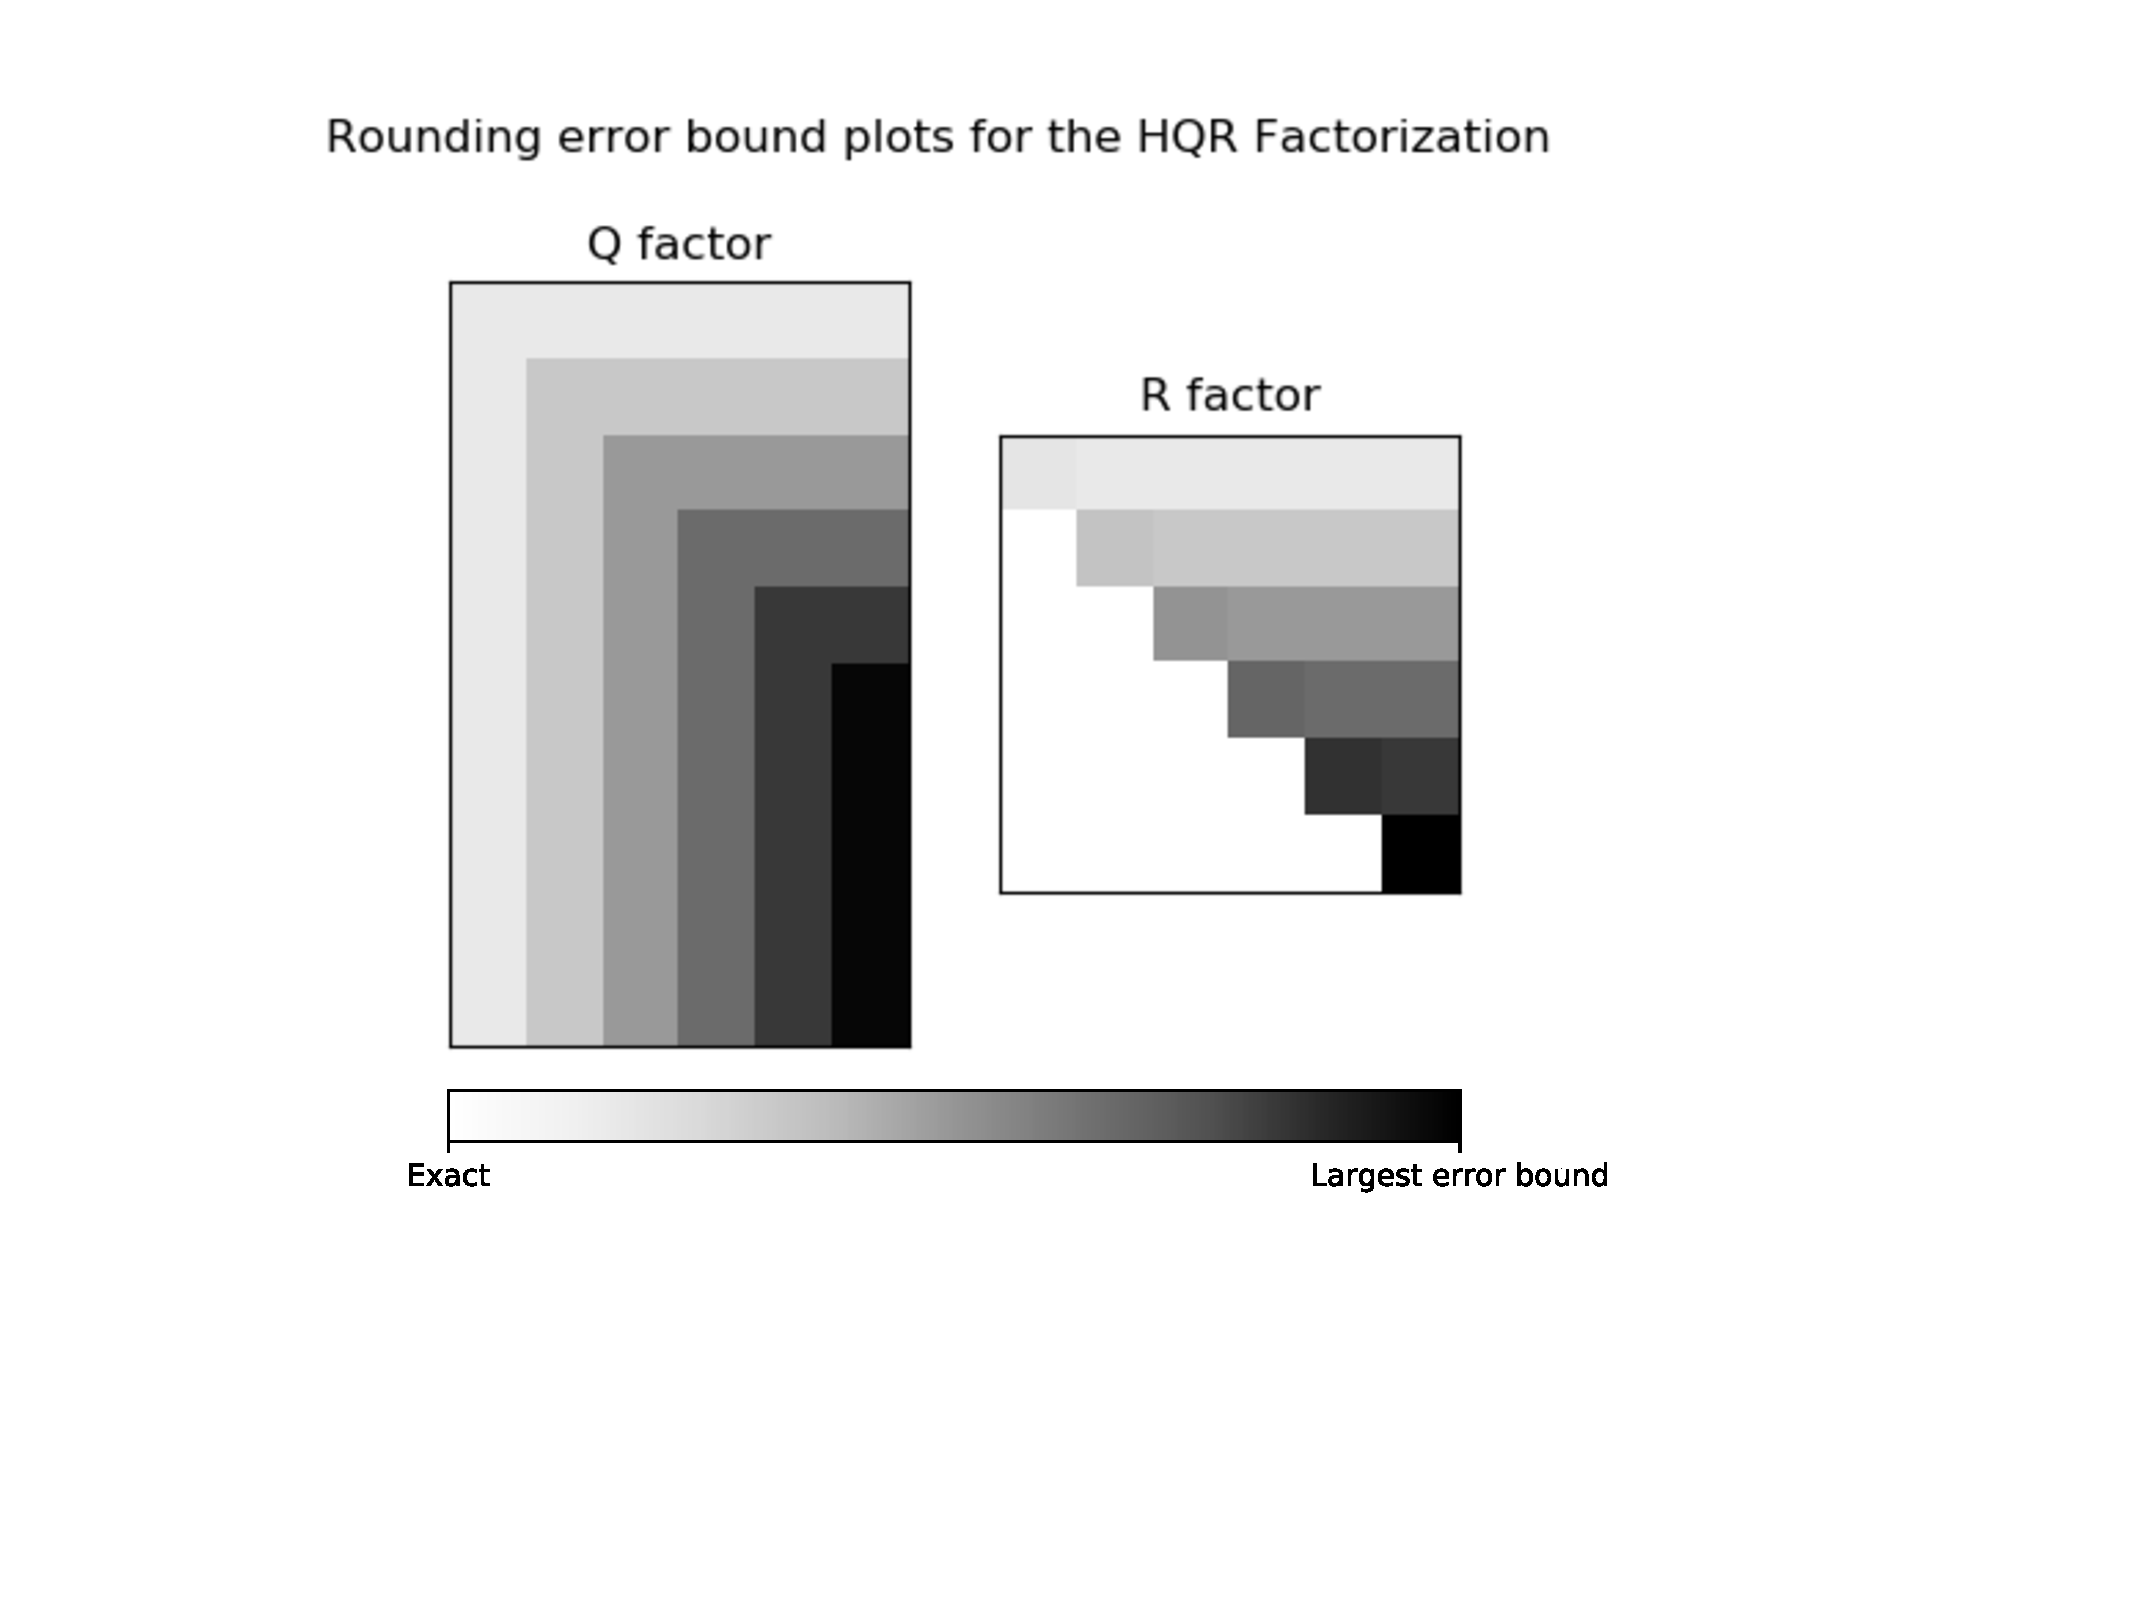
\includegraphics[width=0.5\textwidth]{./figures/figure2.pdf}
%%% 	\end{center}
%%% 	\caption{\label{fig:QRerr} Grayscale representation of distribution of rounding errors bounds for the HQR algorithm.}% Elements $\hat{\bb{R}}_{ij}=(1+\tth_w^{(r_{ij})})\bb{R}_{ij}$ and $\hat{\bb{Q}}_{ij}=(1+\tth_w^{(q_{ij})})\bb{Q}_{ij}$, where $r_{ij}$ and $q_{ij}$ are represented by grayscale.}	
%%% 	%\end{figure}
%%% \end{wrapfigure}

Consider a thin QR factorization where $\bb{A}\in\R^{m\times n}$ for $m\geq n$, we have $\bb{Q}\in\R^{m\times n}$ and $\bb{R}\in\R^{n\times n}$.
The pseudo-algorithm in Section \ref{sec:HQRf} shows that each succeeding Householder transformation is applied to a smaller lower right submatrix each time. \par
%For the $\bb{R}$ factor, everything beneath the diagonal is set to zero and therefore is exact, but all other elements incur rounding errors.
%These elements ($\hat{\bb{R}_{ii}}$ for $i\leq j$) go through $i-1$ Householder transformations designed to zero out $A^{(0)}[1:m, 1], A^{(1)}[2:m, 2], \cdots, A^{(i-2)}[i-1:m, i-1]$ that correspond to vectors of length $m, \cdots, m-(i-1)$.
%In addition, diagonal elements ($\hat{\bb{R}_{ii}}$) are then assigned $\hat{\sigma}$ from the process of zeroing out $A^{(i-1)}[i:m, i]$.
%Rounding errors for the $\bb{Q}$ factor can be formulated similarly. 
%Since the $i^{th}$ Householder transformation in building $\bb{Q}$ is performed on the $[i:m, i:n]$ lower-right submatrix, elements in $Q[i:m,i]$ and $Q[i,i:n]$ go through $i$ Householder transformations corresponding to vectors of sizes $m-(n-1), \cdots, m-(n-i)$ for $i = 1, \cdots, n$.

%Consequently, rounding error bounds for each element of $\bb{R}$ and $\bb{Q}$ can be specifically computed by its location within the matrices, as is displayed in Figure~\ref{fig:QRerr} for a $10$-by-$6$ example.
Instead of continuing with a componentwise analysis of how accumulated rounding errors are distributed by HQR, we transition into normwise error analyses.
To do this, we use the analysis from the preceding section (summarized in Equation~\ref{eqn:applyP}) to implicitly form the matrix norm error of the Householder transformation matrix, $\bb{P_v}$.
Then, we use the result of Lemma 3.7 in \cite{Higham2002} to get a normwise bound on the perturbation effect of multiple matrix multiplications.
This result is summarized in Theorem~\ref{thm:feHQR}, and the proof is detailed extensively in \ref{Appendix:HQR}.
%Then, we use the number of Householder transformations a column of $\bb{A}$ goes through to be transformed into a column of $\bb{R}$, and implicitly find the matrix norm error of the $\bb{Q}^{\top}$ that is formed in the process.
%Note that columnwise norms are easily converted to matrix norms (c.f. Lemma 6.6 in\cite{Higham2002}). 

\begin{theorem}
	\label{thm:feHQR}
	Let $\bb{A}\in\R^{m\times n}$ with $m\geq n$ have full rank, $n$. 
	Let $\hat{\bb{Q}}\in\R^{m\times n}$ and $\hat{\bb{R}}\in\R^{n\times n}$ be the thin QR factors of $\bb{A}$ obtained via the HQR algorithm with a mixed-precision scheme as is outlined in Assumption~\ref{assump:mp}.
	Let $d=\lfloor\frac{(m-1) u_s}{u_w}\rfloor$, and $z=1$ or $z=2$. 
	Then we have normwise forward error bounds
	\begin{align}
	\hat{\bb{R}} &= \bb{R} + \bb{\Delta R} = \hat{\bb{P}}_n\cdots\hat{\bb{P}}_1 \bb{A},\\
	\hat{\bb{Q}} &= \bb{Q} + \bb{\Delta Q} = \hat{\bb{P}}_1\cdots\hat{\bb{P}}_n \bb{I},
	\end{align}
	where
	\begin{equation}
	  \|\bb{\Delta Q}\|_F \leq n^{3/2} \tilde{\gamma}_w^{(6d+6z+13)},
	\end{equation}
	and for column $j$ in $\{1, \cdots, n\}$,
	\begin{equation}
	\|\bb{\Delta R}[:,j]\|_2 \leq j\tilde{\gamma}_w^{(6d+6z+13)}\|\bb{A}[:,j]\|_2.
	\end{equation}
	We also form a backward error.
	Let $\bb{A}+\bb{\Delta A} = \hat{\bb{Q}}\hat{\bb{R}}$, where $\hat{\bb{Q}}$ and $\hat{\bb{R}}$ are obtained via Algorithm~\ref{algo:hhQR}.
	Then,
	\begin{equation}
	\|\bb{\Delta A}\|_F \leq n^{3/2}\tilde{\gamma}_w^{(6d+6z+13)}\|\bb{A}\|_F.
	\end{equation}
\end{theorem}

\subsubsection{HQR Comparison to Uniform Precision Analysis}
\label{sec:mpupHQRcomparison}
%Contributions from the mixed-precision inner product scheme on the results from Theorem~\ref{thm:feHQR} are shown directly at the level of a single Householder transformation, as shown in Equation~\ref{eqn:applyP}.
The mixed-precision segments of the analysis behind Theorem~\ref{thm:feHQR} derive from the mixed-precision inner product scheme outlined in Assumption~\ref{assump:mp} and are propagated to form the error bounds for a single Householder transformation as is shown in Equation~\ref{eqn:applyP}.
All steps to form the error bounds in Theorem~\ref{thm:feHQR} from the error bound for a single Householder transformation (Equation~\ref{eqn:applyP}) directly follow the analyses in Section 19.3 of \cite{Higham2002}.
In these steps, we generalize the single Householder transformation error bound, 
\begin{equation}
\fl(\bb{P}_{\bb{v}}\bb{x})= (\bb{P}_{\bb{v}} + \bb{\Delta P_{v}})\bb{x},\qquad \|\bb{\Delta P_v}\|_F \leq \epsilon,\label{eqn:applyPgen}
\end{equation}
for some small quantity $0<\epsilon\ll 1$, and propagate it through the for-loop in Algorithm~\ref{algo:hhQR}. 
This process then results in forward error bound coefficients $n\epsilon$ or $n^{3/2}\epsilon$.
Since this $\epsilon$ value remains constant, the rounding error analysis for both mixed-precision and uniform-precision schemes are essentially the same with different values for $\epsilon$.
The uniform precision equivalent of Equation~\ref{eqn:applyP} is shown in Equation~\ref{eqn:applyPup},
\begin{equation}
\fl(\bb{P}_{\bb{v}}\bb{x})= (\bb{P}_{\bb{v}} + \bb{\Delta P_{v}})\bb{x},\qquad \|\bb{\Delta P_v}\|_F \leq \tilde{\gamma}^{(m)},
\label{eqn:applyPup}
\end{equation}
which is derived in detail in \cite{Higham2002}.
Therefore, we only need to compare $\gamma^{(6d+6z+13)}$ against $\gamma^{(cm)}$, where $c$ is a small integer. 
Although $d$ relies on both $m$ and the precisions $w$ and $s$, we can generally assume that $cm\gg (6d+6z+13)$ in most mixed-precision settings.
%, where $c$ is a small integer constant. 
Therefore, the new bounds in Theorem~\ref{thm:feHQR} are much tighter than the existing ones and more accurately describe the kind of rounding error accumulated in mixed-precision computational settings.
%up to the level of a single Householder transformation as is shown in Equation~\ref{eqn:applyP}.
%
%All steps to form the error bounds in Theorem~\ref{thm:feHQR} from the error bound for a single Householder transformation (c.f. Equation~\ref{eqn:applyP}) result in coefficients of $\tilde{\gamma}_w^{(6d+6z+13)}$, and these steps directly follow the analyses in Section 19.3 of \cite{Higham2002}.
%In these steps, we generalize the single Householder transformation error bound, 
%\begin{equation}
%\fl(\bb{P}_{\bb{v}}\bb{x})= (\bb{P}_{\bb{v}} + \bb{\Delta P_{v}})\bb{x},\qquad \|\bb{\Delta P_v}\|_F \leq \epsilon,\label{eqn:applyPgen}
%\end{equation}
%for some small quantity $0<\epsilon\ll 1$, and propagate it through the for-loop in Algorithm~\ref{algo:hhQR}. 
%Since this $\epsilon$ value remains constant, the rounding error analysis for both mixed-precision and uniform-precision schemes are essentially the same with different values for $\epsilon$.
%Therefore, we only need to compare $\gamma^{(6d+6z+13)}$ against $\tilde{\gamma}^{(m)}$. 
%Although $d$ relies on both $m$ and the precisions $w$ and $s$, we can generally assume that $m\gg (6d+6z+13)$ in most mixed-precision settings. 
%Therefore, new bounds in Theorem~\ref{thm:feHQR} are much tighter than the existing ones, and more accurately describe the kind of rounding error accumulated in mixed-precision computational settings.
%\section{Tall-and-Skinny QR}
\label{sec:TSQR}
	Some important problems that require QR factorizations of overdetermined systems include least squares problems, eigenvalue problems, low rank approximations, as well as other matrix decompositions.
	Although Tall-and-Skinny QR (TSQR) broadly refers to row-block QR factorization methods, we will discuss a specific variant of TSQR which is also known as the AllReduce algorithm \cite{Mori2012}.
	In this paper, the TSQR/AllReduce algorithm refers to the most parallel variant of all row-block QR factorization algorithms discussed in \cite{Demmel2012}.
	A detailed description and rounding error analysis of this algorithm can be found in \cite{Mori2012}, and we present a pseudocode for the algorithm in Algorithm~\ref{algo:par_tsqr}.
	Our initial interest in this algorithm came from its parallelizable nature, which is particularly suitable to implementation on GPUs. 
	Additionally, our numerical simulations (discussed in Section~\ref{sec:NE}) show that TSQR can not only increase the speed but also outperform the traditional HQR factorization in low precisions.
	\subsection{TSQR/AllReduce Algorithm}
		Algorithm~\ref{algo:par_tsqr} takes a tall-and-skinny matrix, $\bb{A}$, and organizes it into row-blocks. 
		HQR factorization is performed on each of those blocks, and pairs of $\bb{R}$ factors are combined  to form the next set of $\bb{A}$ matrices to be QR factorized. 
		This process is repeated until only a single $\bb{R}$ factor remains, and the $\bb{Q}$ factor is built from all of the Householder constants and vectors stored at each level.
		The most gains from parallelization can be made in the initial level where the maximum number of independent HQR factorizations occur. 
		Although more than one configuration of this algorithm may be available for a given tall-and-skinny matrix, the number of nodes available and the shape of the matrix eliminate some of those choices. 
		For example, a 1600-by-100 matrix can be partitioned into 2, 4, 8, or 16 initial row-blocks but may be restricted by a machine with only 4 nodes, and a 1600-by-700 matrix can only be partitioned into 2 initial blocks.
		%The choice in the initial partition determine the recursion depth which we call level.
		Our numerical experiments show that the choice in the initial partition, which directly relates to the recursion depth of TSQR, has an impact in the accuracy of the QR factorization. \par
		%Our numerical experiments provide some insight into how to make this decision in an optimal way.  \par
		
		We refer to \emph{level} as the number of recursions in a particular TSQR implementation. 
		An $L$-level TSQR algorithm partitions the original matrix into $2^L$ submatrices in the initial or $0^{th}$ level of the algorithm, and $2^{L-i}$ QR factorizations are performed in level $i$ for $i = 1 , \cdots, L$. 
		The set of matrices that are QR factorized at each level $i$ are called $\bb{A}_j^{(i)}$ for $j = 1, \cdots, 2^{L-i}$, where superscript $(i)$ corresponds to the level and the subscript $j$ indexes the row-blocks within level $i$.
		%Note that each $\bb{A}_i^{(j)}$ is created from combining two $\bb{R}$ factors in the previous level, $i-1$.
		%,  $\bb{A}$ matrices that are QR factorized.
		%The initial row-blocks that partition the original matrix is the initial or $0^{th}$ level of the algorithm, and each successive set of $\bb{A}_i^{(j)}$ matrices (created from combining $\bb{R}$ factors of the previous level) are referred to as first level, second level, and so forth.
		%The subscript, $i$ corresponds to the level, and the superscript $(j)$ indexes the row-blocks within level $i$.
		In the following sections, Algorithm~\ref{algo:par_tsqr} ({\tt tsqr}) will find a TSQR factorization of a matrix $A\in\R^{m\times n}$ where $m \gg n$. 
		The inline function {\tt qr} refers to Algorithm~\ref{algo:hhQR}, {\tt hh\_mult} is Algorithm~\ref{algo:hh_mult}, and we use Algorithm ~\ref{algo:hh_v2} as a subroutine of {\tt qr}.

%		performs a HQR factorization and returns $\bb{V} \in \R^{m\times n}$, $\bm{\beta}\in\R^{n}$, and $\bb{R} \in R^{n\times n}$.
%		For $i=1,\cdots,n$, the $i^{th}$ column of $\bb{V}$ and $\bm{\phi}_i$ are the Householder vector and constant that defines the $i^{th}$ Householder transformation matrix, $\bb{P}_i$ for the QR decomposition of the input matrix. 
%		The columns of $\bb{V}$ are the Householder vectors (first component normalized to $1$) that can form the matrix $\bb{Q}_{\text{thin}} = \bb{P}_1 \cdots \bb{P}_nI_{m\times n}$.
%		Note that a full $\bb{Q}$ can be constructed via $\bb{Q}_{\text{full}}=\bb{P}_1\cdots \bb{P}_n$. 
%		
%		
%		Algorithm~\ref{algo:hh_mult} is the implementation of multiplying  $\bb{Q}:= \bb{P}_1 \cdots \bb{P}_n$ to another matrix or vector, when only the householder vectors to construct $\bb{P}_i$'s are given. This takes advantage of the special property of householder matrices-- $\bb{P}_i$'s are rank-one updates of the identity. let $\bb{B}\in\R^{m\times d}$. The straightforward mod of  computing $\bb{Q}\bb{B}$ costs $\mathcal{O}(m^2d)$ where the costs of constructing $\bb{Q}$ itself is ignored. However,  Algorithm ~\ref{algo:hh_mult} describes a method that is only $\mathcal{O}(mnd)$. 

		\subsubsection{TSQR Notation}
		We will introduce new notation due to the multi-level nature of the TSQR algorithm.
		In the final task of constructing $\bb{Q}$, $\bb{Q}_j^{(i)}$ factors are aggregated from each block at each level.
		Each $\bb{Q}_j^{(i)}$ factor from level $i$ is partitioned such that two corresponding $\bb{Q}^{(i-1)}$ factors from level $i-1$ can be applied to them. 
		The partition (approximately) splits $\bb{Q}_{j}^{(i)}$ into two halves, $[\tilde{\bb{Q}}_{j, 1}^{(i)\top} \tilde{\bb{Q}}_{j, 2}^{(i)\top}]^{\top}$.
		% \(\bb{Q}_{j}^{(i)} = \begin{bmatrix}
		%\tilde{\bb{Q}}_{j, 1}^{(i)}\\ 
		%\tilde{\bb{Q}}_{j, 2}^{(i)} 
		%\end{bmatrix},\)
		The functions $\alpha(j)$ and $\phi(j)$ are defined such that $\bb{Q}_j^{(i)}$ is applied to $\tilde{\bb{Q}}_{\alpha(j), \phi(j)}^{(i+1)}$.
		For $j = 1 , \cdots, 2^{L-i}$ at level $i$, we need $j = 2(\alpha(j)-1) + \phi(j)$, where $\alpha(j) = \lceil \frac{j}{2}\rceil$ and $\phi(j) = 2 + j - 2\alpha(j)$.
%		\begin{itemize}
%			\item $\alpha(j) = \lceil \frac{j}{2}\rceil $ and
%			\item $\phi(j) = 2 + j - 2\alpha(j)$.
%		\end{itemize} 
		Section~\ref{Qdetails} shows full linear algebra details for a single-level ($L=1$, $2$ initial blocks) example.
		The reconstruction of $\bb{Q}$ can be implemented more efficiently (see \cite{BDGJNS2014}), but the reconstruction method in Algorithm~\ref{algo:par_tsqr} is presented for a clear, straightforward explanation.
		
		\subsubsection{Single-level Example}
		\label{Qdetails}
		In the single-level version of this algorithm, we first bisect $\bb{A}$  into $\bb{A}_1^{(0)}$ and $\bb{A}_2^{(0)}$ and compute the QR factorization of each of those submatrices.
		We combine the resulting upper-triangular matrices , i.e.,  \(\bb{A}_{1}^{(1)} =\begin{bmatrix}
		\bb{R}_{1}^{(0)}\\ 
		\bb{R}_{2}^{(0)} 
		\end{bmatrix},\)   which is QR factorized, and the process is repeated:
		\[
		\bb{A} = \begin{bmatrix}
		\bb{A}_1^{(0)}\\
		\bb{A}_2^{(0)}
		\end{bmatrix} = \begin{bmatrix}
		\bb{Q}_1^{(0)}\bb{R}_1^{(0)}\\
		\bb{Q}_2^{(0)}\bb{R}_2^{(0)}
		\end{bmatrix} = \begin{bmatrix}
		\bb{Q}_1^{(0)} & \bb{0}\\
		\bb{0} & \bb{Q}_2^{(0)}
		\end{bmatrix} \begin{bmatrix}
		\bb{R}_1^{(0)} \\
		\bb{R}_2^{(0)}
		\end{bmatrix} =\begin{bmatrix}
		\bb{Q}_1^{(0)} & \bb{0}\\
		\bb{0} & \bb{Q}_2^{(0)}
		\end{bmatrix} \bb{A}_1^{(1)} =\begin{bmatrix}
		\bb{Q}_1^{(0)} & \bb{0}\\
		\bb{0} & \bb{Q}_2^{(0)}
		\end{bmatrix} \bb{Q}_1^{(1)}\bb{R}.%_1^{(1)}
		\] 
		The $\bb{R}$ factor of $\bb{A}_1^{(1)}$ is the final $\bb{R}$ factor of the QR factorization of the original matrix, $\bb{A}$. 
		However, the final $\bb{Q}$ still needs to be constructed.
		Bisecting  $\bb{Q}_1^{(1)}$ into two submatrices, i.e. $\tilde{\bb{Q}}_{1,1}^{(1)}$ and $\tilde{\bb{Q}}_{1,2}^{(1)}$, allows us to write and compute the product more compactly,  \[
	    \bb{Q}:=\begin{bmatrix}
		\bb{Q}_1^{(0)} & \bb{0}\\
		\bb{0} & \bb{Q}_2^{(0)}
		\end{bmatrix} \bb{Q}_1^{(1)} =    \begin{bmatrix}
		\bb{Q}_1^{(0)} & \bb{0}\\
		\bb{0} & \bb{Q}_2^{(0)}
		\end{bmatrix} \begin{bmatrix}
		\tilde{\bb{Q}}_{1,1}^{(1)}\\
		\tilde{\bb{Q}}_{1,2}^{(1)}
		\end{bmatrix}= \begin{bmatrix}
		\bb{Q}_1^{(0)}\tilde{\bb{Q}}_{1,1}^{(1)} \\ 
		\bb{Q}_2^{(0)}\tilde{\bb{Q}}_{1,2}^{(1)}
		\end{bmatrix}. \]
		More generally, Algorithm~\ref{algo:par_tsqr} takes a tall-and-skinny matrix $\bb{A}$ and level $L$ and finds a QR factorization by initially partitioning $\bb{A}$ into $2^L$ row-blocks and includes the building of $\bb{Q}$.
		
		\begin{algorithm2e}[H]
			\DontPrintSemicolon % Some LaTeX compilers require you to use \dontprintsemicolon instead
			\KwIn{$\bb{A}\in\R^{m \times n}$ where $m \gg n$, $L\leq\lfloor\log_2\left(\frac{m}{n}\right)\rfloor$, and $2^L$ is the initial number of blocks. }
			
			\KwOut{$\bb{Q}\in\R^{m \times n}$, $\bb{R} \in\R^{n\times n}$ such that 	$\bb{Q}\bb{R} = \bb{A}$.}
			$h \gets \lfloor \frac{m}{2^L} \rfloor$ \tcp*{Number of rows for all but the last block.}
			$r \gets m - (2^L-1)h$ \tcp*{Number of rows for the last block ($h\leq r <2h$).}
			\tcc{Split $\bb{A}$ into $2^L$ blocks. Note that level $(i)$ has $ 2^{L-i}$ blocks.}
			\For {$j = 1 : 2^L-1$}{
				$\bb{A}_j^{(0)} \gets \bb{A}[(j-1)h+1: jh, :]$ %\bb{I}_{(j-1)h, jh}^{\top}\bb{A}$
			}
			$\bb{A}_{2^L}^{(0)} \gets \bb{A}[(2^L-1)h:m, :]$ \tcp*{Last block may have more rows.} %\bb{I}_{(2^L-1)h, m}^{\top}\bb{A}
			\tcc{Store Householder vectors as columns of matrix $\bb{V}_j^{(i)}$, Householder constants as components of vector $\bm{\beta}_j^{(i)}$, and set up the next level.}
			\For{$i = 0 : L-1$}{
				\tcc{The inner loop can be parallelized.}
				\For {$j = 1 : 2^{L-i}$ }{
					$\bb{V}_{2j-1}^{(i)}$, $\bm{\beta}_{2j-1}^{(i)}$, $\bb{R}_{2j-1}^{(i)} \gets{\tt qr}(\bb{A}_{2j-1}^{(i)})$ \;
					$\bb{V}_{2j}^{(i)}$, $\bm{\beta}_{2j}^{(i)}$, $\bb{R}_{2j}^{(i)} \gets{\tt qr}(\bb{A}_{2j}^{(i)})$\;
					% \tcp*{$\bb{V}_j^{(i)} \in \R^{2n\times n}$ for $i > 0$ and $\bb{R}_j^{(i)} \in \R^{n\times n}$ always.} 
					\(\bb{A}_{j}^{(i+1)} \gets \begin{bmatrix}
					\bb{R}_{2j-1}^{(i)}\\
					\bb{R}_{2j}^{(i)}
					\end{bmatrix}\)
				}
			}
			\tcc{At the bottom-most level, get the final $\bb{R}$ factor.}
			$\bb{V}_{1}^{(L)}$, $\bm{\beta}_1^{(L)}$, $\bb{R}  \gets{\tt qr}(\bb{A}_{1}^{(L)})$ \;
			$\bb{Q}_{1}^{(L)} \gets {\tt hh\_mult}(\bb{V}_{1}^{(L)}, I_{2n\times n})$\;
			\tcc{Compute $\bb{Q}^{(i)}$ factors by applying $\bb{V}^{(i)}$ to $\bb{Q}^{(i+1)}$ factors.}
			%\tcc{Combine $\bb{Q}$ factors from bottom-up-- look at Notation (4).}
			\For {$i = L-1 : -1 : 1$}{
				\For {$j = 1 : 2^{L-i}$}{
					\(\bb{Q}_{j}^{(i)} \gets {\tt hh\_mult}\left(\bb{V}_{j}^{(i)}, \begin{bmatrix}
					\tilde{\bb{Q}}_{\alpha(j), \phi(j)}^{(i+1)}\\
					\bb{0}_{n,n}
					\end{bmatrix}\right)\)
					%\bb{Q}_{j}^{(i)} \gets $ {\tt hh\_mult} $(\bb{V}_{j}^{(i)}, [\tilde{\bb{Q}}_{\alpha(j), \phi(j)}^{(i+1)}; O_{n,n}])$
				}
			}
			\tcc{At the top-most level, construct the final $\bb{Q}$ factor.}% from $\bb{Q}^{0}$ factors.}
			$\bb{Q} \gets [];$\;
			\For{$ j = 1 : 2^L $}{
				\(\bb{Q} \gets \begin{bmatrix}
				\bb{Q} \\
				{\tt hh\_mult}\left(\bb{V}_{j}^{(0)} , \begin{bmatrix}
				\tilde{\bb{Q}}_{\alpha(j), \phi(j)}^{(1)}\\
				O_{\tilde{h},n}
				\end{bmatrix} \right)
				
				\end{bmatrix}\)
			}
			\Return{$\bb{Q}$, $\bb{R}$}
			\caption{$\bb{Q},\bb{R}={\tt tsqr}(\bb{A}, L)$.  Finds a QR factorization of a tall, skinny matrix, $\bb{A}$. }
			\label{algo:par_tsqr}
		\end{algorithm2e}
	\subsection{TSQR Rounding Error Analysis}
	\label{sec:TSQRre}
The TSQR algorithm presented in Algorithm~\ref{algo:par_tsqr} is a divide-and-conquer strategy for the QR factorization that uses the HQR within the subproblems. 
Divide-and-conquer methods can naturally be implemented in parallel and accumulate less rounding errors.
For example, the single-level TSQR decomposition of a tall-and-skinny matrix, $\bb{A}$ requires 3 total HQRs of matrices of sizes $\lfloor\log_{2}(\frac{m}{n})\rfloor$-by-$n$, $\lceil\log_{2}(\frac{m}{n})\rceil$-by-$n$, and $2n$-by-$n$.
The single-level TSQR strictly uses more FLOPs, but the dot product subroutines may accumulate smaller rounding errors (and certainly have smaller upper bounds) since they are performed on shorter vectors, and lead to a more accurate solution overall.
These concepts are elucidated in \cite{Mori2012}, where the rounding error analysis of TSQR is shown in detail in \cite{Mori2012}.
We summarize the main results from \cite{Mori2012} in Theorem~\ref{thm:moriTSQR}.
	
%		\begin{figure}[ht]
%			\centering
%			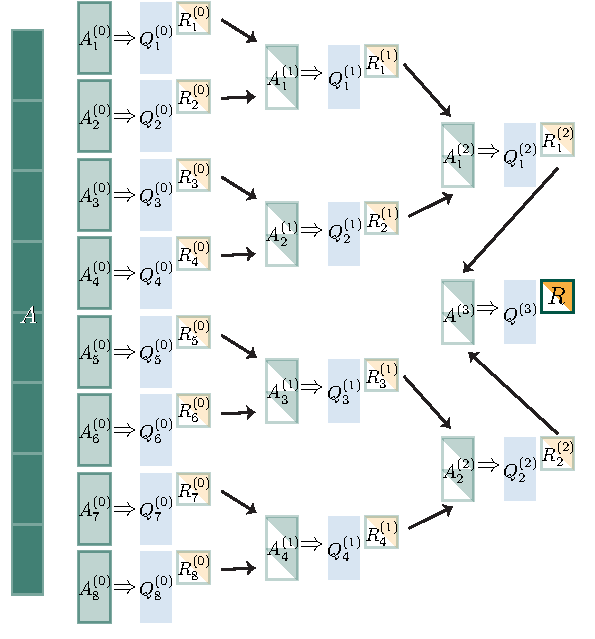
\includegraphics{./figures/TSQR.pdf}
%			\caption{\label{fig:TSQR} Visualization of the TSQR factorization (AllReduce) algorithm.}	
%		\end{figure}
		
		%\subsubsection{Variants of TSQR}
			


%Since the subroutine with leading order FLOPs of an HQR implementation is the dot product, and we will use it to approximate the computational complexity of the TSQR algorithm.
%For a tall-and-skinny matrix $\bb{A}\in\R^{m\times n}$ where $m\gg n$, the deepest possible TSQR scheme has $\lfloor\log_{2}(\frac{m}{n})\rfloor$ levels of recursion. 
%The general idea is that deeper levels of recursion lead to shorter dot products, but more FLOPs over all, and both of these factors contribute to the accumulation of rounding errors and its effect on the accuracy of the QR factorization.
\begin{theorem}
	\label{thm:moriTSQR}
	Let $\bb{A}\in\R^{m\times n}$ with $m\geq n$ have full rank, $n$, and $\hat{\bb{Q}}\in\R^{m\times n}$ and $\hat{\bb{R}}\in\R^{n\times n}$ be the thin QR factors of $\bb{A}$ obtained via Algorithm~\ref{algo:par_tsqr}. 
	Then we have normwise forward error bounds
	\begin{align*}
	\hat{\bb{A}} = \bb{A} +\bb{\Delta A} &=  \bb{Q}(\bb{R} + \bb{\Delta R}),\\
	\hat{\bb{Q}} &= \bb{Q} + \bb{\Delta Q},
	\end{align*}
	where
	\begin{align}
	\|\bb{\Delta R}\|_F, \|\bb{\Delta A}\|_F &\leq \left[n\tilde{\gamma}_{ \frac{m}{2^L}}+(1+n\tilde{\gamma}_{ \frac{m}{2^L}})\left\{(1+n\tilde{\gamma}_{ 2n})^L-1\right\}\right]\|\bb{A}\|_F, \text{ and} \label{eqn:tsqrRA}\\
	\|\bb{\Delta Q}\|_F &\leq \sqrt{n}\left[(1+n\tilde{\gamma}_{ \frac{m}{2^L}})(1+n\tilde{\gamma}_{ 2n})^L -1\right].\label{eqn:tsqrQ}
	%& \leq \left[n\tilde{\gamma}_{ \frac{m}{2^L}}+(1+n\tilde{\gamma}_{ \frac{m}{2^L}})\left\{(1+n\tilde{\gamma}_{ 2n})^L-1\right\}\right]\|\bb{A}\|_F,\label{eqn:tsqrA}
	\end{align}
	Furthermore, if we assume $n\tilde{\gamma}_{ \frac{m}{2^L}}, n\tilde{\gamma}_{ 2n} \ll 1$, the coefficient for $\|\bb{A}\|_F$ in Equations~\ref{eqn:tsqrRA} can be approximated as
	\begin{equation}
	\left[n\tilde{\gamma}_{ \frac{m}{2^L}}+(1+n\tilde{\gamma}_{ \frac{m}{2^L}})\left\{(1+n\tilde{\gamma}_{ 2n})^L-1\right\}\right] \simeq n\tilde{\gamma}_{ \frac{m}{2^L}} + Ln\tilde{\gamma}_{ 2n}, %(46) in Mori
	\end{equation}
	and the right hand side of Equation~\ref{eqn:tsqrQ} can be approximated as
	\begin{equation}
	 \sqrt{n}\left[(1+n\tilde{\gamma}_{ \frac{m}{2^L}})(1+n\tilde{\gamma}_{ 2n})^L -1\right]\simeq \sqrt{n}\left(n\tilde{\gamma}_{ \frac{m}{2^L}} + Ln\tilde{\gamma}_{ 2n}\right). %(67) in Mori
	\end{equation}
	We can also form a backward error, where $\bb{A}+\bb{\Delta \bb{A}_{\text{TSQR}}} = \hat{\bb{Q}}\hat{\bb{R}}$, and both $\hat{\bb{Q}}$ and $\hat{\bb{R}}$ are obtained via Algorithm~\ref{algo:par_tsqr}.
	Then,
	\begin{equation}
	\|\bb{\Delta \bb{A}_{\text{TSQR}}}\|_F =\|\bb{Q \Delta R} + \bb{\Delta Q}\hat{\bb{R}}\|_F \simeq \sqrt{n}\left(n\tilde{\gamma}_{ \frac{m}{2^L}} + Ln\tilde{\gamma}_{ 2n}\right)\|\bb{A}\|_F.
	\end{equation}
\end{theorem}

In Section~\ref{sec:mpupHQRcomparison}, the steps of the HQR algorithm resulted in an error bound of  $\mathcal{O}(\epsilon)$, where the constant is some function with respect to $n$ and where $\epsilon$ is the error bound for a single Householder transformation, described in Equation~\ref{eqn:applyPgen} .
% MATH QUESTION: Can n\epsilon and n^{3/2}\epsilon both be considered as O(\epsilon)?
Similarly, the analysis behind Theorem~\ref{thm:moriTSQR} can be generalized via defining $\epsilon_1$ to be the error bound for a single Householder transformation corresponding to the vector length at the initial level $0$, $\frac{m}{2^L}$, and defining $\epsilon_2$ to be the error bound for a Householder transformation corresponding to vector length in all deeper levels,  $2n$.
This generalization leads to the error bound coefficients
\begin{align}
 n\epsilon_1 + Ln\epsilon_2& \qquad\text{for}\quad  \|\bb{\Delta Q}\|_F, \|\bb{\Delta \bb{A}_{\text{TSQR}}}\|_F,\\
 \sqrt{n}(n\epsilon_1+Ln\epsilon_2)& \qquad\text{for}\quad \|\bb{\Delta R}\|_F, \|\bb{\Delta A}\|_F.
\end{align}

In a uniform-precision setting, these correspond to
\begin{equation}
\epsilon_1 = \tilde{\gamma}^{(\frac{m}{2^L})}\quad \text{and}\quad \epsilon_2 = \tilde{\gamma}^{(2n)},
\end{equation}
and in the mixed-precision setting outlined in Assumption~\ref{assump:mp}, they correspond to
\begin{equation}
\epsilon_1 = \gamma_w^{(6d_1+6z+13)}, \quad \text{and } \epsilon_2 = \gamma_w^{(6d_2+6z+13)},
\end{equation}
where $d_1 := \lfloor{(\frac{m}{2^L}-1)\frac{u_s}{u_w}\rfloor}$ and $d_2 :=\lfloor \frac{(2n-1)u_s}{u_w}\rfloor$ respectively.
In both settings, we see that increasing $L$ may decrease $\epsilon_1$, but may still increase the overall bounds; the larger $L$ still could have an adverse effect on the coefficients in Theorem~\ref{thm:moriTSQR}.
This trade-off is precisely the balance between the sizes of initial blocks and the number of levels in the TSQR algorithm, and an optimal TSQR scheme would ideally minimize $\epsilon_1$ and $\epsilon_2$ with the choice of $L$.
These error bounds are studied in detail in the following section. %Section ~\ref{sec:HTSQR}.
%, resulting in some sort of a trade-off balance between , 
%While the original problem required forming the QR decomposition of a $m$-by-$n$ matrix, an $L$-level TSQR solves $2^L$ QR factorizations of $\lfloor\frac{m}{2^L}\rfloor$-by-$n$ matrices in Level $0$, followed by $2^{L-1}, \cdots, 2^{0}$ QR factorizations of $2n$-by-$n$ matrices in levels $1$ to $L$, which sums to $2^{L}-1$ QR factorizations of $2n$-by-$n$ matrices. 

\subsubsection{HQR and TSQR error bound comparison}
\label{sec:HTSQR}
We compare the error bounds for HQR and TSQR algorithms. 
\paragraph{Uniform precision comparison}Consider the larger error bounds in the uniform precision equivalents of Theorems~\ref{thm:feHQR} and \ref{thm:moriTSQR}, which are the bounds of $\bb{\Delta Q}$ and $\bb{\Delta A}$. 
In order for the a meaningful TSQR error bound to outperform the bound for the HQR algorithm, we need integers $m, n > 0$, and $L\geq0$ such that,
\begin{equation*}
1\gg n^{3/2}\gamma^{(m)} \gg n^{3/2}(\gamma^{(\frac{m}{2^L})}+L\gamma^{(2n)}).
\end{equation*}
If we assume $\frac{m}{2^L}=2n$, the HQR bound is $\frac{L+1}{2^L}$ larger than the bound for TSQR with $L$ levels. 
For example, in single precision, a HQR of a $2^{15}$-by-$2^6$ matrix results in an upper bound relative backward error ($\|\bb{A}-\hat{\bb{Q}}\hat{\bb{R}}\|_F/\|\bb{A}\|_F$) of $\approx${\tt1.002}, but a TSQR with $L=8$ is bounded by $\approx${\tt 3.516e-02}. 
This case exemplifies a situation in which stability is not guaranteed in HQR, but the method is stable when using TSQR, even in the worst-case. 
Now consider some $2^{20}$-by-$2^{12}$ matrix and QR factorizations performed with double precision.
The error bound for HQR is {\tt 1.686e-7}, whereas the error bound for TSQR with 12 levels is {\tt 5.351e-10}.
In general, we can conjecture that values of $L$ that can make $m2^{-L}$ and $2Ln$ much smaller than $m$, should produce a TSQR that outperforms HQR in worst-case scenarios, at least in uniform precision settings.
However, the range of matrix sizes that TSQR can accommodate decreases as $L$ grows larger.
%, and the range is only half of that of HQR even for a single-level TSQR. 
Figure~\ref{fig:paramspace} shows the matrix sizes HQR, 2-level TSQR, and 4-level TSQR can accommodate as well as their respective error bounds.\par
\begin{wrapfigure}{l}{.45\textwidth}
	\centering
	%\vspace{-15pt}
	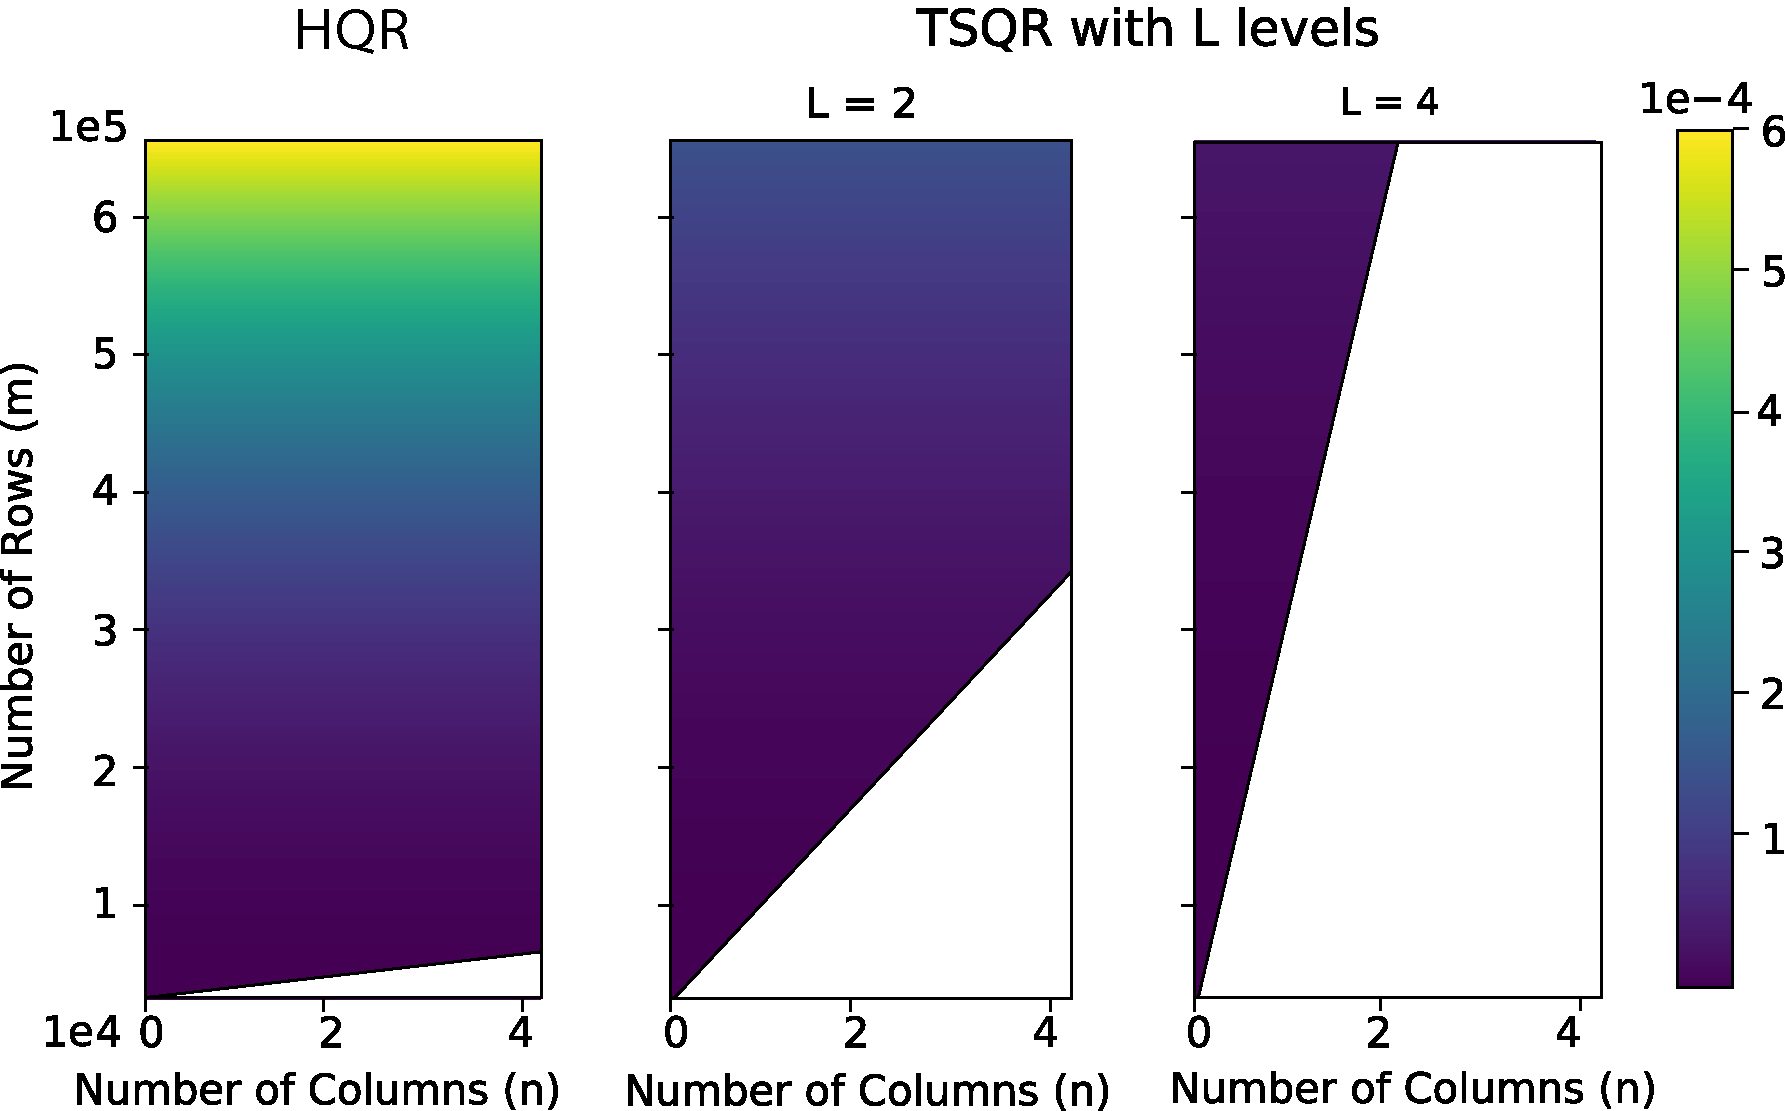
\includegraphics[width=.45\textwidth]{./figures/paramspace.png}
	\caption{\label{fig:paramspace} Non-white space indicates allowable matrix sizes for each scheme, and color map represents error bounds for $\|\bb{\Delta Q}\|_F$ for uniform precision error analysis when using double precision arithmetic.}
	\vspace{-10pt}	
\end{wrapfigure}
\paragraph{Mixed precision comparison}Consider a mixed-precision setting such as in Assumption~\ref{assump:mp}, and we assume $u_p=u_w$, so that $z=2$.
In order for the a meaningful TSQR error bound to outperform the bound for the HQR algorithm, we now need integers $m, n > 0$, and $L\geq 0$ such that
\begin{equation*}
1\gg n^{3/2}\gamma_w^{(6d + 25)} \gg n^{3/2}(\gamma_w^{(6d_1+ 25)}+L\gamma_w^{(6d_2+ 25)}),
\end{equation*}
where $d=\lfloor\frac{(m-1) u_s}{u_w}\rfloor$, $d_1 = \lfloor{(\frac{m}{2^L}-1)\frac{u_s}{u_w}\rfloor}$, and $d_2 =\lfloor \frac{(2n-1)u_s}{u_w}\rfloor$. 

In contrast to the analysis for uniform precision settings, large $L$ values do not necessarily reduce the error bounds of TSQR. 
While large $L$ can imply $m\gg m2^{-L}+2Ln$, it does not always lead to $d \gg d_1+Ld_2$.
Although the theoretical error bounds do not give a clear indication of the worst-case performances of HQR and TSQR in mixed-precision settings, TSQR outperformed HQR on ill-conditioned matrices within our numerical simulations.

These experiments are discussed in detail in the next section.%Section~\ref{sec:NE}.



\subsection{Numerical Experiment}
\label{sec:NE}
%\subsection{Single Precision}
In Section~\ref{sec:HTSQR}, we theorized that conditions exist where TSQR could outperform HQR and that these conditions were hard to identify in mixed-precision settings. 
An empirical comparison of these two QR factorization algorithms in double precision can be found in \cite{Mori2012}, where they conclude that deeper TSQR tends to produce more accurate QR factorizations than HQR.
However, using TSQR with deep levels (large $L$) can actually start to perform worse than TSQR with shallower levels (smaller $L$), since deeper levels require more FLOPs.
We instead focused on comparing HQR and TSQR performances in a mixed-precision setting.
Our numerical simulations show that TSQR can still outperform HQR in low, mixed-precision settings in practice even though the theoretical bounds do not guarantee stability.
%are all $\mathcal{O}(10)$ (c.f. Table~\ref{table:HTSQRerr}), and get larger as we go from HQR to TSQR, and larger as we increase $L$. 
Our empirical results do not behave as the theoretical bounds suggest, and even show opposite trends at times. 
This discrepancy highlights the shortcomings of deterministic error bounds that are too pessimistic. \par
%showed that there exists conditions in which the worst-case rounding error bound for TSQR can be expected to be smaller than that of HQR. 
%These conditions are met more easily in high, uniform-precision settings than low mixed-precision settings.
%The success of TSQR in high, uniform-precision settings is explored and discussed in \cite{Mori2012}, where they conclude that the computed relative error, $\|\hat{\bb{Q}}\hat{\bb{R}}-A\|_F$, tends to decrease as they increase $L$, but only up to a certain point.
%This may appear to contradict our conclusion in Section~\ref{sec:upHTSQR}, where we found that as long as $\frac{L}{2^{L-1}}\ll 1$, there e 
%\subsubsection{Experiment Details}
We used Julia v1.0.4 for all of the numerical simulations. 
This programming language allows half precision storage as well as {\tt castup} and {\tt castdown} operations to and from single and double precisions, but has no half precision arithmetic.
Therefore, we relied on using Algorithm~\ref{algo:simulate} for $f\in \text{OP} \cup\{{\tt dot\_product}\}$ to simulate half and mixed-precision arithmetic operations. 
%Specifically, we approximated , and 
%To simulate the mixed-precision setting described in Assumption~\ref{assump:mp} with $u_p = 0$ (which implies $z=1$), we used Algorithm~\ref{algo:simulate} for the dot product routine.
%That is, for $\bb{x}_{\text{half}},\bb{y}_{\text{half}}\in\F_{\text{half}}^m$, we approximated $\fl(\bb{x}_{\text{half}}^{\top}\bb{y}_{\text{half}})$ with {\tt simHalf}$(${\tt dot\_product} $, \bb{x}_{\text{half}}, \bb{y}_{\text{half}})$ to simulate mixed-precision dot products.
%We used Algorithm~\ref{algo:simulate} for all other operations as well to simulate half precision arithmetic.
For HQR, we created a mixed-precision version of the LAPACK routine xGEQRF, where the dot product subroutine was approximated by $\fl(\bb{x}_{\text{half}}^{\top}\bb{y}_{\text{half}})$ with {\tt simHalf}$(${\tt dot\_product} $, \bb{x}_{\text{half}}, \bb{y}_{\text{half}})$ to simulate the mixed-precision setting described in Assumption~\ref{assump:mp} with $u_p = 0$ (which implies $z=1$), and we used Algorithm~\ref{algo:simulate} on all other basic operations in OP to simulate half/storage precision arithmetic. 
%Using these simulated operations as subroutines for 
%By using these simulated half and mixed precision versions of basic operations at subroutines for our implementation of the LAPACK routine xGEQRF, we 
%To implement half and mixed-precision simulations within HQR, we wrote our own versions of it that almost replicates LAPACK routine xGEQRF, where the disparity only comes from the storage format of the information required to build the $\bb{Q}$ factor. 
This HQR was then used as a subroutine of TSQR as well. 
There are cases where the rounding will differ between the mixed-precision setting and the way we mimic it, i.e., basic operations that are meant to be in half/storage precision arithmetic, but are instead casted up to single and back down, as the tiebreaker within correct rounding may lead to different results than true half/storage precision arithmetic. 
All in all, our experiments nearly replicated the mixed-precision setting we assumed for the error analysis in Sections~\ref{sec:HQRre} and \ref{sec:TSQRre}.\par 
%Although we kept the matrix size constant, we varied the condition numbers of these matrices by the method described below.
%We speculated that matrices with larger condition numbers would behave closer to the ``worst-case scenario'' with respect to rounding errors.
%Table~\ref{table:HTSQRerr} shows the theoretical error bounds from Section~\ref{sec:HQRre} and \ref{sec:TSQRre} that correspond to the conditions of our experiment.
%Stability is not guaranteed for any of these QR factorization methods. 
%
%\begin{table}[h]
%	\centering
%	\begin{tabular}{||c|c|c|c|c|c|c|c||} 
%		\hline
%		$L$ & $0$ & $1$ & $2$ & $3$ & $4$ & $5$ & $6$ \\ \hline
%		$n^{3/2}(\gamma_w^{(6d_1+ 25)}+L\gamma_w^{(6d_2+ 25)})$ & {\tt 9.36} & {\tt 18.73} & {\tt 28.09} & {\tt 37.46} & {\tt 46.82} & {\tt 56.19} & {\tt 65.55}\\ \hline
%	\end{tabular}
%	\caption{Error bounds for when $m=4000$, $n=100$, $u_w=u_{\text{half}}$, $u_s={\text{single}}$, and $d_1,d_2$ are defined in Section~\ref{sec:TSQRre}. Error bound for HQR is recovered when $L=0$.}
%	\label{table:HTSQRerr}
%\end{table}

%\paragraph{Constructing Test Matrices}
Following example from \cite{Mori2012}, we used $m$-by-$n$ random matrices, $\bb{A}_{\alpha}$, constructed via
\begin{equation}
\bb{A}_{\alpha} = \bb{Q'}(\alpha \bb{E} + \bb{I})/\|\bb{Q'}(\alpha \bb{E} + \bb{I})\|_F,
\label{eqn:genRM}
\end{equation}
where $\bb{Q'}\in\mathbb{R}^{m\times n}$ is a random orthogonal matrix and $\bb{E}\in\R^{n\times n}$ is the matrix of $1$'s. 
The random orthogonal matrix $\bb{Q'}$ is generated by taking a QR factorization of an iid $4000$-by-$100$ matrix sampled from $Unif(0,1)$, and we used the built-in QR factorization function in Julia.
By construction, $\bb{A}_{\alpha}$ has 2-norm condition number $n\alpha+1$. 
By varying $\alpha$ from {\tt 1e-4} to {\tt 1}, we varied the condition number from $1.1$ to $101$, and we generated $10$ samples for each value of $\alpha$.

%\subsubsection{Results}


We generated random matrices of size $4000$-by-$100$ using Equation~\ref{eqn:genRM} and computed their HQR and TSQR for $L=1, \cdots, 6$ in a mixed-precision setting that simulates Assumption~\ref{assump:mp} with $z=1$.
The relative backward error, $\|\hat{\bb{Q}}\hat{\bb{R}}-\bb{A}\|_F/\|\bb{A}\|_F$, was computed by casting up $\hat{\bb{Q}}$, $\hat{\bb{R}}$, and $\bb{A}$ to double precision to compute the Frobenius norms.
Note that the mixed-precision HQR error bounds $n\tilde{\gamma}_{w}^{(6d+6z+13)}$ and $n^{3/2}\tilde{\gamma}_{w}^{(6d+6z+13)}$ for $m=4000$ and $n=100$ are {\tt 0.936} and {\tt 9.364} respectively, and the mixed-precision TSQR bounds for $L=1,\cdots, 5$  are even larger, which indicates that our error bounds do not guarantee stability.\par

\begin{wrapfigure}{l}{.4\textwidth}
	\centering
	\vspace{-10pt}
	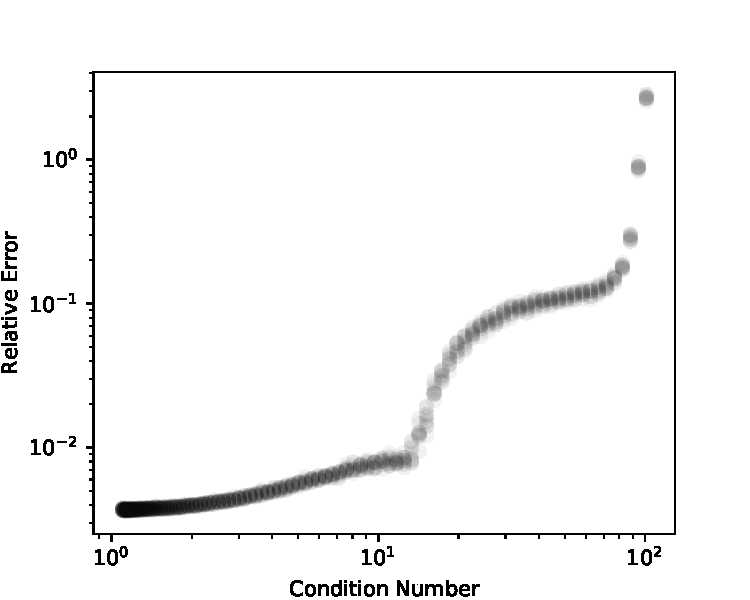
\includegraphics[width=.4\textwidth]{./figures/unblocked.pdf}
	\caption{\label{fig:unblocked} HQR errors for matrices with varying condition numbers.}
	%\vspace{-10pt}	
\end{wrapfigure}
Figure~\ref{fig:unblocked} shows the backward errors of mixed precision HQR increasing as the theoretical condition numbers of the generated random matrices increase, and these errors correspond to the error data on the vertical axis, $L=0$, of Figure~\ref{fig:allTSQR}.
In addition to the errors from HQR, Figure~\ref{fig:allTSQR} shows the errors from mixed precision TSQR of levels varying from $L=1$ to $L=5$, where each line represents the errors of HQR and variants of TSQR calculated from the same random test matrix.
Figure~\ref{fig:allTSQR} reveals two different trends for the errors as we deepen the complexity of the QR algorithm from HQR to TSQR with 5 levels. 
One trend occurs for matrices with smaller condition numbers, where HQR and all levels of TSQR are stable, but deepening the levels of TSQR worsens the errors. 
The other trend occurs for matrices with higher condition numbers, where single-level and 2-level TSQR yield smaller errors than HQR. 
In these cases, TSQR with 3 or more levels have errors similar to or worse than 2-level TSQR, but those errors tend to not rise above the HQR errors.
These results suggests that TSQR can significantly outperform HQR even in mixed-precision settings, and particularly when HQR is unstable due to larger condition numbers.
Although this experiment focused on condition numbers, identifying other properties that point to better performance of TSQR than HQR can further broaden the potential use of mixed-precision TSQR in applications.
%The first trend When the error is low enough for the unblocked QR factorization, TSQR performs worse for these matrices.
%Recall that machine precision for half-precision is about $10^{-3}$. 
%This shows that the traditional QR factorization had been very good to begin with.
%Finally, even when TSQR is \textit{successful} initially, we can see that too many initial blocks can become a problem as well. 
%
%Overall, this figure shows a variety of results that encourage further exploration. 
%We have shown that TSQR can improve on certain matrices where the unblocked HQR algorithm was highly unstable in half-precision.
%Identifying which matrix properties correlate to TSQR and why can help broaden the possibility of using lower precision arithmetic for QR factorizations.

\begin{figure}[h!]%{r}{.53\textwidth}
	\centering
	%\vspace{-10pt}
	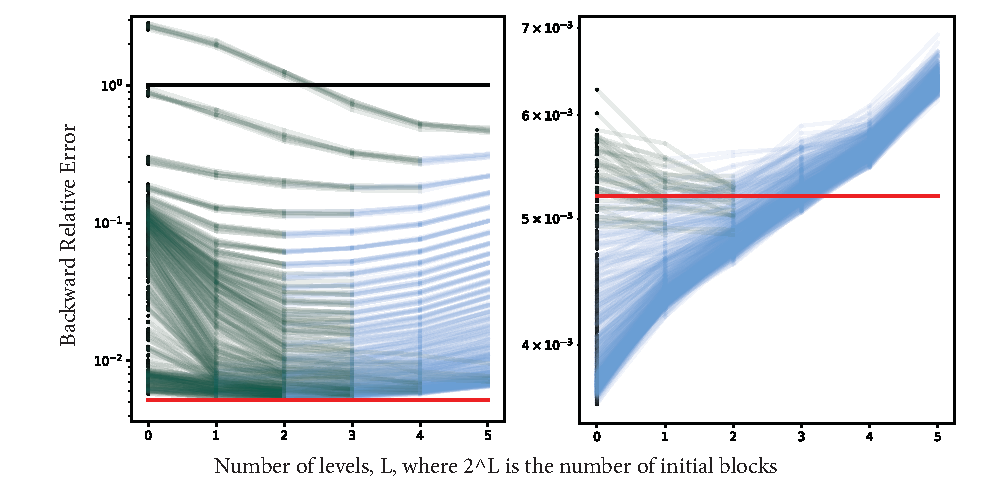
\includegraphics[width=0.8\textwidth]{./figures/allTSQR2.pdf}
	\caption{\label{fig:allTSQR} Left plot shows the relative error of QR factorization for matrices with condition numbers ranging from 5.3 to 101, and the right plot shows the errors for matrices with condition numbers ranging from 1.1 to 5.3. }
	\vspace{-10pt}
\end{figure} 

%\section{Applications}
\label{sec:Apps}
Many applications in scientific computing typically employ double precision when lower precision may actually be sufficient. 
Due to the advances in processors, FLOPs are now considered free, causing bandwidth and storage to be the computational bottleneck. 
With the emergence of new technology that supports low precision and the need to reduce bandwidth and storage concerns, interest in mixed-precision algorithms has reemerged. 
%However, identifying which applications can tolerate lower precision and still achieve sufficient results is a challenging task that wasn't particularly relevant prior to the emergence of new technology that supports low precision.

Since low and mixed precision settings benefit from speed-up and reduced storage, applications that process large amounts of data are potential candidates for this research.
Here, we discuss our results from applying our mixed-precision HQR as a subroutine of an iterative eigensolver in the context of spectral clustering.\par

\paragraph{Graph partitioning} A graph is defined by a set of nodes and a set of edges between the nodes.
Partitioning, or clustering, is a task that seeks communities within a graph such that nodes within a community are \emph{more similar} to each other than to nodes outside of that community. 
In datasets where the true communities are known, we can use pairwise-precision and pairwise-recall (see \cite{GraphChallenge})  which are defined in Definition~\ref{def:P&R}) to evaluate the accuracy of a clustering task.
\begin{definition}
	\label{def:P&R}
	%Some relevant evaluation metrics of classification of clustering tasks are precision and recall. 
	%Precision is the fraction of relevant instances among the retrieved instances.
    Pairwise-precision and pairwise-recall are measured by checking for every pair of nodes if the pair is classified into the same cluster (positive), or else (negative).
	\begin{equation}
	\text{Precision} = \frac{\#\text{True Positive}}{\#\text{True Positive}+\#\text{False Positive}}, 
	\qquad
	%%% \end{equation} 
	%Recall is the fraction of relevant instances that have been retrieved over the total amount of relevant instances.
	%%% \begin{equation}
	\text{Recall} = \frac{\#\text{True Positive}}{\#\text{True Positive}+\#\text{False Negative}}.
	\end{equation}
\end{definition}

\subsection{Spectral Graph Clustering}
\label{sec:cluster}
Some spectral clustering methods utilize identifying $k$ dominant eigenvectors of a similarity matrix of a graph, which then can be used to identify $k$ clusters. 
Another potential use of iterative eigensolvers for spectral clustering is in identifying the second smallest eigenvalue and its eigenvector pair, called the Fiedler value and vector.
%Whether convergence to the Fiedler vector is quick or not is more uncertain than in identifying dominant eigenvectors.
In addition, many eigenproblems outside of spectral clustering only require finding a few eigen pairs.
This family of problems tends to admit tall-and-skinny matrix structures and could utilize TSQR as well. 
We will use subspace iteration, a variant of the power method defined in Algorithm~\ref{algo:subIter} that uses a QR factorization of a tall-and-skinny matrix at each iteration and that quickly converges to the dominant eigenvectors.
Although we only experimented with comparing mixed-precision HQR to uniform precision HQR, TSQR could also be used in this application. 
\par

\subsubsection{Subspace Iteration}
Subspace iteration is a modification of the power method, which computes an invariant subspace with dimension $p > 1$ (see \cite{Bai2000}).
A variant of this algorithm is shown below in Algorithm~\ref{algo:subIter}.

\begin{algorithm2e}
	\DontPrintSemicolon % Some LaTeX compilers require you to use \dontprintsemicolon instead
	\KwIn{Adjacency matrix $\bb{A}\in\{0, 1\}^{m \times m}$ where $m \geq n$, {\tt max\_iter}, the maximum number of iterations, $\tau$ the threshold for the eigenspace error, and $k$, the suspected number of clusters.}
	\KwOut{$\bb{Q}$}
	Initialize $\bb{Y}\in \mathbb{R}^{m\times k}$, a random matrix.
	\tcp{$Y$ would likely be full-rank.} 
	$\bb{Q}, \bb{R}\gets \tt{qr}(\bb{Y})$ 
	\For{$i=1, \cdots,$ {\tt max\_iter}}{
		$\bb{Y} \gets \bb{AQ}$\;
		\If{$\frac{\|\bb{Y}-\bb{QQ}^{\top}\bb{Y}\|_2}{\|\bb{Y}\|_2} < \tau$}{exit loop. \tcp{$\|\bb{Y}-\bb{QQ}^{\top}\bb{Y}\|_2$ is the eigenspace error.}}
		$\bb{Q, R} \gets {\tt qr}(\bb{Y})$
	}
	\Return $\bb{Q}$
	\caption{$\bb{Q}=$ {\tt subIter}$(\bb{A}, \text{\tt max\_iter}, \tau, k)$. Find orthogonal basis (given by columns of output matrix $Q$) of an invariant subspace of the input adjacency matrix, $A$.}
	\label{algo:subIter}
\end{algorithm2e}
This algorithm is an iterative method with two possible stopping criteria: 1) the maximum number of iterations to complete before exiting the loop is declared as max\_iter, or 2) if the eigenspace error is smaller than $\tau$, then exit the loop.
In practice, we added a third stopping criterion in the case that the declared $\tau$ value was too small, which would force an exit from the loop when the eigenspace error began to increase.

\subsubsection{Density-based Spatial clustering of Applications with Noise (DBSCAN)}
DBSCAN is a density-based spatial clustering algorithm introduced in \cite{EKSX1996} and is widely used in practice.
This algorithm only requires input data, location of nodes, and two parameters, radius of neighborhoods and minimum number of points required to form a dense region. 
The two parameters for the DBSCAN algorithm were tuned to provide the best result, given that we used the same set of parameters for the entire experiment.

\subsection{Experiment Details and Results}
Our main goal in this experiment was to test if the eigenspaces identified by lower precision HQR could produce sufficient graph partitioning. 
We used subspace iteration (Algorithm~\ref{algo:subIter}) to identify eigenspaces, DBSCAN to partition the embedding of the nodes onto these eigenspaces, and precision and recall to evaluate clustering performances. 
We used a static graph of $5000$ nodes  with $19$ known true partitions for the Graph Challenge \cite{GraphChallenge}, which are derived from block stochastic matrices. 
The graphs we used were undirected and unweighted; the only elements in the adjacency matrices were $0$'s and $1$'s, which can easily be represented in half, single, and double precision floats. 
For $i=1, \cdots, 10$, let $\bb{Y}_{\text{half},i}\in\F_{\text{half}}^{5000\times 19}$ be the half precision storage of the $i^{th}$ random matrix.
Since any half precision float can be exactly represented in single and double precisions, $\bb{Y}_{\text{half},i}$'s can be easily cast up to single and double precisions, $\bb{Y}_{\text{single},i}$ and $\bb{Y}_{\text{double},i}$.
We performed mixed-precision HQR within subspace iteration initialized by $\bb{Y}_{\text{half},i}$'s, and uniform-precision HQR for subspace iteration initialized by $\bb{Y}_{\text{single},i}$'s  and $\bb{Y}_{\text{double},i}$'s.
For trial $i = 1, \cdots, 10, $ we repeated the following steps.
\begin{enumerate}[Step 1.]
	\item Identify an orthogonal basis of dimension 19 (number of known true partitions) with subspace iteration using the appropriate HQR routine for $\bb{Y}_{\text{half},i}$, $\bb{Y}_{\text{single},i}$ and $\bb{Y}_{\text{double},i}$.
	\item Apply DBSCAN to the output matrices of previous step to cluster most nodes into communities and the remaining nodes as outliers. 
	\item Measure clustering performances of DBSCAN on the three different precision subspace iteration embeddings using precision and recall.
\end{enumerate}

\paragraph{Subspace Iteration Results} 
\begin{wrapfigure}{r}{.5\textwidth}
	\centering
	%\vspace{-10pt}
	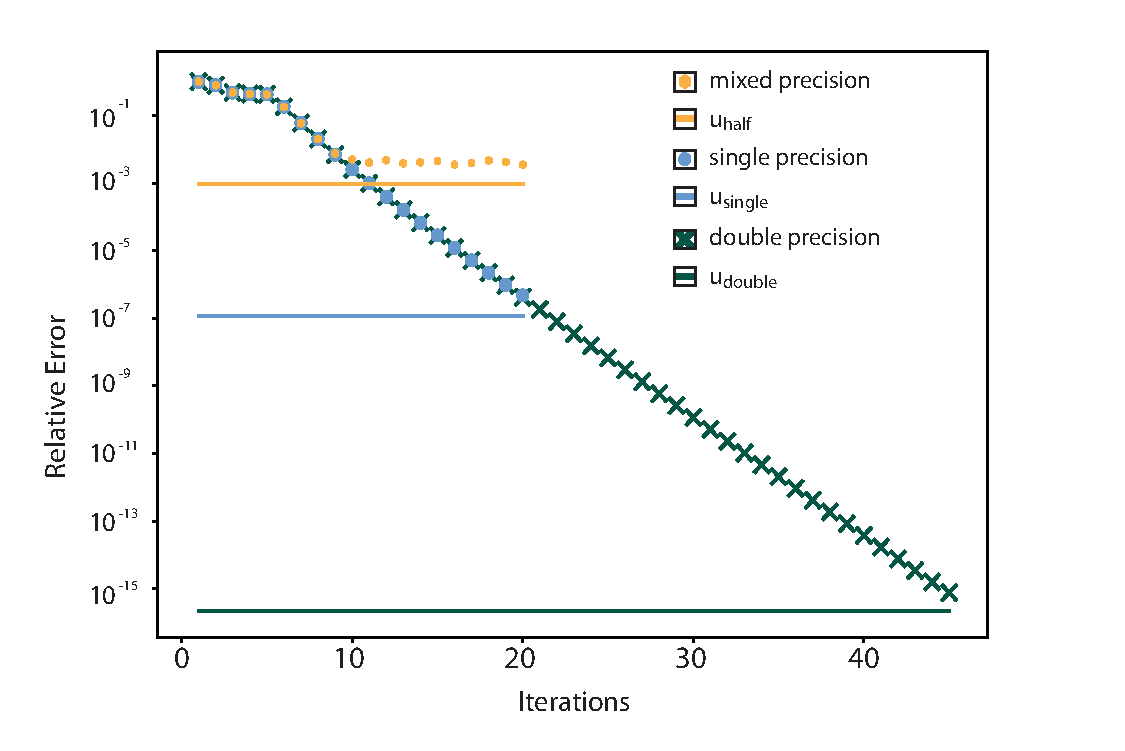
\includegraphics[width=.5\textwidth]{./figures/5000-19subIter.pdf}
	\caption{\label{fig:subIter} Eigenspace Error for subspace iteration with using double-, single-, and half- precision traditional Householder QR factorizations.}
	\vspace{-20pt}	
\end{wrapfigure}
Figure~\ref{fig:subIter} shows the eigenspace error, $\|\bb{Y}-\bb{QQ}^{\top}\bb{Y}\|_2/\|\bb{Y}\|_2$, from the subspace iteration step of one trial.
The stopping criteria, $\tau$, were set to $5u_{\text{single}}$ and $5u_{\text{double}}$ for the uniform precision HQRs and $5u_{\text{half}}$ for the mixed-precision HQR.
The solid lines are plotted to show the unit round-off values. 
The uniform precision implementations of subspace iterations reached their stopping criterion set by $\tau$, and the mixed-precision implementation fluctuated close to but never dipped below $\tau$. 
The convergence rate was approximately the same across the three different implementations, which suggests that the lower precision routines (mixed-precision HQR or uniform single precision HQR) can be used as a preconditioner for the double precision solution, and if paired with appropriate hardware could lead to increased computational efficiency.
In addition, if double precision eigenspace error is not necessary to achieve sufficient clustering results, we can simply use the lower precision HQR subspace iterations as full eigensolvers. 

\paragraph{Clustering Results} 
Table~\ref{table:PR} shows the worst-case precision and recall results from the $10$ trials for each subspace iteration implementation. 
The DBSCAN algorithm and the calculation of precision and recall were computed in double precision, and the variance in precision and recall values for these $10$ trials were in the range of {\tt 1e-6}.
Subspace iteration that employs lower precision HQR results in a suboptimal solution to the basis, which has a larger loss in orthogonality when compared to the solution from subspace iteration that uses higher precision HQR. 
However, clustering results show minimal difference in the precision and recall and suggests that a lower precision HQR within subspace iteration can still lead to a sufficiently accurate clustering. 
%Possible future works include trying different clustering methods for Step 2. 
\begin{table}[h!]
	\centering
%%% 	\begin{tabular}{ |c|c|c| } 
%%% 		\hline
%%% 		HQR scheme & Precision & Recall \\ \hline 
%%% 		mixed-precision & {\tt 0.9822} & {\tt 0.9393} \\ 
%%% 		single-precision & {\tt 0.9817} & {\tt 0.9407} \\ 
%%% 		double-precision &{\tt 0.9822} & {\tt 0.9405}\\
%%% 		\hline
%%% 	\end{tabular}
\begin{tabular}{ |c|c|c|c| }
\hline
HQR Scheme & Mixed Precision & Single Precision & Double Precision \\ \hline
Prec / Recall & 
{\tt 0.9822} / {\tt 0.9393} &
{\tt 0.9817} / {\tt 0.9407} &
{\tt 0.9822} / {\tt 0.9405} \\
\hline
\end{tabular}
	%%% \caption{\label{table:PR} Minimum (worst-case) precision and recall values for $10$ trials of DBSCAN on graph with $5000$ nodes and $19$ true clusters.}
	\caption{\label{table:PR} Minimum (worst-case) precision and recall for $10$ trials on graph with $5000$ nodes and $19$ true clusters.}
\end{table}
% and calls for further investigations into a variable precision approach to other spectral clustering methods as well.
%The mixed-precision implementation approached its best performance close to $10$ iterations, and continued to fluctuate near there without hitting the $\tau$ value. 
%Nonetheless, we can see that the first $9$ iterations of the subspace iteration technique yielded the same eigenspace errors for all three precisions. 
%The same pattern continued for single- and double- precision implementations until they reached single-precision unit round-off near $10^{-7}$, and the double-precision unit round-off near $10^{-15}$. 
%Therefore, we can do with lower-precision QR factorizations that require less storage and faster computation time if low-precision eigenspace error is sufficient for spectral clustering.
%Due to the random element of the initial matrix $\bb{Y}$ at the beginning of subspace iteration, there is some variability to its performance in identifying an invariant subspace. 
%In addition, we chose the number of columns of $\bb{Y}$ to be the number of true clusters, which is usually unknown in practice.
%\subsubsection{Results}
%We used the $5000$ node static graph from \cite{GraphChallenge}, but varied the clustering results by using $10$ different random matrices as the initial $\bb{Y}$.
%Therefore, for each HQR scheme (uniform double, uniform single, and mixed-precision) $10$ different initializations

\section{Conclusion}
Though the use of lower precision naturally reduces the bandwidth and storage needs, the development of GPUs to optimize low precision floating point arithmetic have accelerated the interest in half precision and mixed-precision algorithms. 
%the interest in half precision and mixed-precision algorithms that demonstrate speedier times, lower energy consumption, and lower memory usage. 
Loss in precision, stability, and representable range offset for those advantages, but these shortcomings may have little to no impact in some applications.
It may even be possible to navigate around those drawbacks with algorithmic design. \par 

The existing rounding error analysis cannot accurately bound the behavior of mixed-precision arithmetic.
We have developed a new framework for mixed-precision rounding error analysis and applied it to HQR, a widely used linear algebra routine, and implemented it in an iterative eigensolver in the context of spectral clustering. 
The mixed-precision error analysis builds from the inner product routine, which can be applied to many other linear algebra tools as well.
The new error bounds more accurately describe how rounding errors are accumulated in mixed-precision settings.
We also found that TSQR, a communication-avoiding, easily parallelizable QR factorization algorithm for tall-and-skinny matrices, can outperform HQR in mixed-precision settings for ill-conditioned, extremely overdetermined cases, which suggests that some algorithms are more robust against lower precision arithmetic.
As QR factorizations of tall-and-skinny matrices are common in spectral clustering, we experimented with introducing mixed-precision settings into graph partitioning problems.
In particular, we applied DBSCAN to the spectral basis of a graph identified via subspace iteration that used our simulated mixed-precision HQR, which yielded clustering results tantamount to results from employing double-precision entirely.\par

Although this work is focused on QR factorizations and applications in spectral clustering, the mixed precision round-off error analysis can be applied to other tasks and applications that can benefit from employing low precision computations. 
While the emergence of technology that support low precision floats combats issues dealing with storage, now we need to consider how low precision affects stability of numerical algorithms. 
%TODO: Talk about stability?

Future work is needed to test larger, more ill-conditioned problems with different mixed-precision settings, and to explore other divide-and-conquer methods like TSQR that can harness parallel capabilities of GPUs while withstanding lower precisions. 

%\appendix
%%Then, $$ \hat{\bb{Q_k}}^{(j)} =  \fl(\hat{\bb{Q_k}}^{(j-1)} \hat{\bb{P}}_{\bb{(k-1)r+j}})= \hat{\bb{Q_k}}^{(j-1)} (\hat{\bb{P}}_{\bb{(k-1)r+j}} +\bb{\Delta}\hat{\bb{P}}_{\bb{(k-1)r+j}}) = \hat{\bb{Q_k}}^{(j-1)}-\fl(\hat{\bb{z_k}}^{(j)})\hat{\bb{v_k}}^{(j)\top}.$$
%%$$ \bb{I} - \hat{\bb{W_k}}^{(j)}\hat{\bb{Y_k}}^{(j)\top} = \bb{I} - \hat{\bb{W_k}}^{(j-1)}\hat{\bb{Y_k}}^{(j-1)\top}-\hat{\bb{z_k}}^{(j)\top}\hat{\bb{v_k}}^{(j)} = (\bb{I} - \hat{\bb{W_k}}^{(j-1)}\hat{\bb{Y_k}}^{(j-1)\top}) \hat{\bb{P}}_{\bb{(k-1)r+j}}$$
%If we can bound $\bb{\Delta P}_{\bb{(k-1)r+j}}$ componentwise, we can use the arguments in the fashion of \cref{eqn:rPs,eqn:rPs-uniform} to quantify the errors accumulated from building the WY representation with the perturbed Householder vectors and constants that result from \cref{algo:hhQR}. 
%
%The only new quantities introduced in the WY representation is the $\bb{W_k}$ factor since $\bb{Y_k}$ is exactly $\bb{V_k}$. 
%Therefore, we only consider  $\bb{z_k}^{(j)} = \beta_k^{(j)}\bb{Q_k}^{(j-1)}\bb{v_j}^{(k)}$.
%We will form  $\tilde{\bb{z_k}}^{(j)} = \fl(\hat{\bb{z_k}}^{(j)})$, the floating point operation computation of $\hat{\bb{z_k}}^{(j)} = \hat{\beta}_k^{(j)}\hat{\bb{Q_k}}^{(j-1)}\hat{\bb{v_j}}^{(k)}$. 
%For now, we assume that $\hat{\bb{Q_k}}^{(j)}$ is a slight perturbation of $\bb{Q_k}^{(j)}$ quantified by $|\bb{\Delta Q_k}^{(j)}|\leq d_1 |\bb{Q_k}^{(j)}|$, $d_1\ll 1$.
%%Since the errors for each column of $\bb{Y_k}$ are represented in \cref{eqn:vbound}, we only need to consider the columns of $\bb{W_k}$, which are 
%%$\bb{z_k}^{(j)} =\beta_k^{(j)}(\bb{I}-\bb{W_k}^{(j-1)}\bb{Y_k}^{(j-1)\top})\bb{v_k}^{(j)}$.
%%An implementation of this computes
%$$\tilde{\bb{z_k}}^{(j)}=\fl\left(\hat{\beta}_k^{(j)}\left(\hat{\bb{v_k}}^{(j)} - \hat{\bb{W_k}}^{(j-1)}\hat{\bb{Y_k}}^{(j-1)\top}\hat{\bb{v_k}}^{(j)}\right)\right),$$
%and we first study the computation of the intermediate term, $\hat{\bb{W_k}}^{(j-1)}(\hat{\bb{Y_k}}^{(j-1)\top}\hat{\bb{v_k}}^{(j)})$.]
%For simplicity, we assume $\hat{\bb{v_k}}^{(j)}$, $\hat{\bb{W_k}}^{(j)}$, and $\hat{\bb{Y_k}}^{(j)}$ all have $m-(k-1)r$ rows. 
%The rounding error incurred in this step is a componentwise error that results from inner products of two different lengths, $m-(k-1)r$ and $j$:
%\begin{align}
%\fl(\hat{\bb{W_k}}^{(j-1)}(\hat{\bb{Y_k}}^{(j-1)\top}\hat{\bb{v_k}}^{(j)})) &=
%(\hat{\bb{W_k}}^{(j-1)}+\bb{\Delta}\tilde{\bb{W_{k}}})(\hat{\bb{Y_k}}^{(j-1)}+\bb{\Delta}\tilde{\bb{Y_{k}}})^{\top}\hat{\bb{v_k}}^{(j)} \\
%&= \hat{\bb{W_k}}^{(j-1)}\hat{\bb{Y_k}}^{(j-1)\top}\hat{\bb{v_k}}^{(j)} + \bb{\Delta d_2} := \tilde{\bb{w_k}} %(1+\tth_{m-(k-1)r})(1+\tth_{j})\hat{\bb{W_k}}^{(j-1)}(\hat{\bb{Y_k}}^{(j-1)\top}\hat{\bb{v_k}}^{(j)}), \\ 
%%&= (1+\tth_{m-(k-2)r})\hat{\bb{W_k}}^{(j-1)}(\hat{\bb{Y_k}}^{(j-1)\top}\hat{\bb{v_k}}^{(j)}).\label{eqn:FLOPwy} \\
%%&= \hat{\bb{W_k}}^{(j-1)}\hat{\bb{Y_k}}^{(j-1)\top}\left(\hat{\bb{v_k}}^{(j)}) + \bb{\Delta}\tilde{\bb{v_{k}}}\right),
%\end{align}
%where $|\bb{\Delta}\tilde{\bb{W_{k}}}| \leq \gamma_{r} |\hat{\bb{W_k}}^{(j-1)}|$ and $|\bb{\Delta}\tilde{\bb{Y_{k}}}| \leq \gamma_{m-(k-1)r} |\hat{\bb{W_k}}^{(j-1)}|$ since $j\leq r$, and $$|\bb{\Delta d_2}|\leq\gamma_{m-(k-2)r} |\hat{\bb{W_k}}^{(j-1)}||\tilde{\bb{Y_k}}{(j-1)\top}| |\hat{\bb{v_k}}^{(j)}|.$$
%Then, 
%\begin{align*}
%\tilde{\bb{z_k}}^{(j)} &= (1+\dd) \hat{\beta}_k^{(j)}\left(\hat{\bb{v_k}}^{(j)} -\tilde{\bb{w_k}}+ \bb{\Delta d_2} \right),\;\; |\bb{\Delta d_3}| \leq u |\hat{\bb{v_k}}^{(j)} -\tilde{\bb{w_k}}| \\
%%&=(1+\dd)\hat{\beta}_k^{(j)}\left(\hat{\bb{v_k}}^{(j)} -\hat{\bb{W_k}}^{(j-1)}\hat{\bb{Y_k}}^{(j-1)\top}\hat{\bb{v_k}}^{(j)} - \bb{\Delta d_1} + \bb{\Delta d_3} \right).  
%%\hat{\bb{W_k}}^{(j-1)}\hat{\bb{Y_k}}^{(j-1)\top}\hat{\bb{v_k}}^{(j)} - \bb{\Delta}\tilde{\bb{w_{k}}}\right)
%\end{align*}
%Since $|- \bb{\Delta d_2} + \bb{\Delta d_3} |\leq u|\hat{\bb{v_k}}^{(j)}
%| +\gamma_{m-(k-2)r} |\hat{\bb{W_k}}^{(j-1)}||\tilde{\bb{Y_k}}{(j-1)\top}| |\hat{\bb{v_k}}^{(j)}|$, we have
%\begin{equation}
%\tilde{\bb{z_k}}^{(j)} = \hat{\bb{z_k}}^{(j)} + \tilde{\Delta}\bb{z_k}^{(j)},\;\; |\tilde{\Delta}\bb{z_k}^{(j)}|\leq \tilde{\gamma}_{m-(k-2)r}|\hat{\bb{z_k}}^{(j)}|.
%\end{equation}
%
%We can finally construct the outer product, $\tilde{\bb{z_k}}^{(j)}\hat{\bb{v_k}}^{(j)\top}$.
%\begin{align*}
%\fl(\tilde{\bb{z_k}}^{(j)}\hat{\bb{v_k}}^{(j)\top}) &= \tilde{\bb{z_k}}^{(j)}(\hat{\bb{v_k}}^{(j)} +\tilde{\Delta}\bb{v_k}^{(j)})^{\top}, \\
%&= \bb{z_k}^{(j)}\bb{v_k}^{(j)\top} + (\tilde{\Delta}\bb{z_k}^{(j)} + \Delta\bb{z_k}^{(j)}) (\hat{\bb{v_k}}^{(j)} +\tilde{\Delta}\bb{v_k}^{(j)})^{\top},
%\end{align*}
%where $|\tilde{\Delta}\bb{v_k}^{(j)})|\leq u|\hat{\bb{v_k}}^{(j)}|$ and $|\Delta\bb{z_k}^{(j)}+\tilde{\Delta}\bb{z_k}^{(j)}| \leq (d_1+\tilde{\gamma}_{m-(k-2)r})|\bb{z_k}^{(j)}|$. 
%Let 
%\begin{align*}
%\Delta \bb{D} &= \fl(\tilde{\bb{z_k}}^{(j)}\hat{\bb{v_k}}^{(j)\top}) - \bb{z_k}^{(j)}\bb{v_k}^{(j)\top}  \\
%&= (\tilde{\Delta}\bb{z_k}^{(j)} + \Delta\bb{z_k}^{(j)}) (\bb{v_k}^{(j)} + \Delta\bb{v_k}^{(j)} +\tilde{\Delta}\bb{v_k}^{(j)})^{\top}.
%\end{align*}
%Since $|\bb{\Delta v_k}^{(j)}|\leq \tilde{\gamma}_{m-(k-1)r}|\bb{v_k}^{(j)}|$, $|\tilde{\Delta}\bb{v_k}^{(j)})+\bb{\Delta v_k}^{(j)}|\leq \tilde{\gamma}_{m-(k-1)r}|\bb{v_k}^{(j)}|$, and we can write 
%$$|\bb{\Delta D}| \leq (\tilde{\gamma}_{m-(k-1)r}+\tilde{\gamma}_{m-(k-2)r}+d_1)|\bb{z_k}^{(j)}||\bb{v_k}^{(j)}|^{\top} = (\tilde{\gamma}_{m-(k-2)r}+d_1)|\bb{z_k}^{(j)}||\bb{v_k}^{(j)}|^{\top}.  $$
%
%
%
%
%
%
%
%
%
% and form $$\hat{\bb{Q_k}}^{(j)} =  \fl(\hat{\bb{Q_k}}^{(j-1)} \hat{\bb{P}}_{\bb{(k-1)r+j}})= \hat{\bb{Q_k}}^{(j-1)} (\hat{\bb{P}}_{\bb{(k-1)r+j}} +\bb{\Delta}\hat{\bb{P}}_{\bb{(k-1)r+j}}) = \hat{\bb{Q_k}}^{(j-1)}-\hat{\bb{z_k}}^{(j)\top}\hat{\bb{v_k}}^{(j)} $$
%
%Therefore, the FLOPs alone from constructing $\fl(\hat{\bb{z_k}}^{(j)})$ with perturbed $\bb{W_k}^{(j-1)}$, $\bb{Y_k}^{(j-1)}$, and $\bb{v_k}^{(j)}$
%Now we delve into how the errors from constructing the previous updates, $\hat{\bb{W_k}}^{(j-1)}$ and $\hat{\bb{Y_k}}^{(j-1)}$, are carried onto the current updates in exact arithmetic.
%We compute
%\begin{align*}
%	\hat{\bb{W_k}}^{(j-1)}(\hat{\bb{Y_k}}^{(j-1)\top}\hat{\bb{v_k}}^{(j)}) &= \sum_{j'=1}^{j-1} \hat{\bb{z_k}}^{(j')}\hat{\bb{v_k}}^{(j')\top}\hat{\bb{v_k}}^{(j)}, \\
%	&= \sum_{j'=1}^{j-1} (\bb{z_k}^{(j')} + \bb{\Delta z_k}^{(j')})(\bb{v_k}^{(j')} + \bb{\Delta v_k}^{(j')})^{\top}(\bb{v_k}^{(j)} + \bb{\Delta v_k}^{(j)}), 
%\end{align*}
%where $|\bb{\Delta v_k}^{(j')}|\leq\tilde{\gamma}_{m-(k-1)r+j'}|\bb{v_k}^{(j')}|$ and $|\bb{\Delta v_k}^{(j)}|\leq\tilde{\gamma}_{m-(k-1)r+j}|\bb{v_k}^{(j)}|$.
%Since $j' < j$, we use \cref{lem:up} and that $j<r$ to result in 
%$$\hat{\bb{v_k}}^{(j')\top}\hat{\bb{v_k}}^{(j)} = \bb{v_k}^{(j')\top}\bb{v_k}^{(j)} + \Delta \bb{v_{k,j}},$$
%where $|\Delta \bb{v_{k,j}}|\leq \tilde{\gamma}_{m-(k-2)r}|\bb{v_k}^{(j')}|^{\top}|\bb{v_k}^{(j)}|$.
%Then, we are left only with the errors in $z_k^{(j')}$'s as shown below:
%\begin{equation}
%\hat{\bb{W_k}}^{(j-1)}(\hat{\bb{Y_k}}^{(j-1)\top}\hat{\bb{v_k}}^{(j)}) = (1+\tilde{\tth}_{m-(k-2)r})\sum_{j'=1}^{j-1} (\bb{z_k}^{(j')} + \bb{\Delta z_k}^{(j')})\bb{v_k}^{(j')\top}\bb{v_k}^{(j)}.
%\end{equation}
%Since the rounding errors from FLOPs shown in \cref{eqn:FLOPwy} are of order only $\tilde{\tth}_{m-(k-1)r}$ and only 2 additional rounding errors are added from the multiplication of $\hat{\beta}_k^{(j)}$ and the vector subtraction, we can state 
%\begin{equation}
%\fl(\bb{z_k}^{(j)}) = (1+\tilde{\tth}_{m-(k-2)r})\beta_k^{(j)}\left(\bb{v_k}^{(j)} - \sum_{j'=1}^{j-1} (\bb{z_k}^{(j')} + \bb{\Delta z_k}^{(j')})\bb{v_k}^{(j')\top}\bb{v_k}^{(j)}\right)\label{eqn:recursiveZ}.
%\end{equation}
%The errors for $\bb{z_k}^{(j')}$'s remain, and we solve for these recursively.
%Note that $\bb{z_k^{(1)}}$ only incurs a single rounding error since it is initialized with $\hat{\beta}_k^{(1)}\hat{\bb{v_k}}^{(1)}$.
%That is, $$\hat{\bb{z_k}}^{(1)}=\bb{z_k}^{(1)}+\bb{\Delta z_k}^{(1)},\;\; |\bb{\Delta z_k^{(1)}}| \leq \tilde{\gamma}_{m-(k-1)r}|\bb{z_k^{(1)}}|,$$
%accounting for $\Delta\beta_k^{(1)}$, $\bb{\Delta v_k}^{(1)}$, and the multiplication operation.
%Using \cref{eqn:recursiveZ} for $j=2$ yields 
%\begin{align}
%\bb{z_k}^{(2)} +\bb{\Delta z_k}^{(2)}  &= (1+\tilde{\tth}_{m-(k-2)r})\beta_k^{(2)}\left(\bb{v_k}^{(2)} -  (\bb{z_k}^{(1)} + \bb{\Delta z_k}^{(1)})\bb{v_k}^{(1)\top}\bb{v_k}^{(2)}\right) \\
%&=(1+\tilde{\tth}_{m-(k-2)r})(1+\tilde{\tth}_{m-(k-2)r})\bb{z_k}^{(2)},
%\end{align}
%where we do not consolidate the two $\tilde{\tth}_{m-(k-2)r}$'s into just one $\tilde{\tth}_{m-(k-2)r}$ under the small integer rule of the tilde notation, since we will continue this recursive relation. 
%At $j=r$, we have 
%\begin{equation}
%\bb{z_k}^{(r)} +\bb{\Delta z_k}^{(r)}= (1+\tilde{\tth}_{m-(k-2)r})^r \bb{z_k}^{(r)}.
%\end{equation}
%
%For simplicity, we assume that the WY representation from the $j-1^{st}$ step is exact to account for only the error accrued in a single update.
%Recall that the $j-1^{st}$ WY representation is
% $$\hat{\bb{Q_k}}^{(j-1)}:=\bb{I}-\hat{\bb{W_k}}^{(j-1)}\hat{\bb{Y_k}}^{(j-1)}=\bb{P_{(k-1)r+1}}\cdots\bb{P_{(k-1)r+j-1}}.$$
%Then, the new update in exact arithmetic is 
%\begin{align*}
%		\bb{I}-\left[\bb{W_k}^{(j)}\fl(\bb{z_k}^{(j)})\right] \left[\bb{Y_k}^{(j)} \hat{\bb{v_k}}^{(j)}\right]^{\top}  & = \bb{Q_k}^{(j-1)} - \fl(\bb{z_k}^{(j)})\hat{\bb{v_k}}^{(j)\top} \\ 
%		&=\bb{Q_k}^{(j-1)}  - \fl(\beta^{(j)}\bb{Q_k}^{(j-1)} \hat{\bb{v_k}}^{(j)})\hat{\bb{v_k}}^{(j)\top},\\
%		&=\bb{Q_k}^{(j-1)} (\bb{P_{(k-1)r+j}} + \Delta \bb{P_{(k-1)r+j}})
%\end{align*}
%which applies the Householder update to the right by applying a rank-1 update.
%We adapt the single left Householder update presented in \cref{lem:19.2} for 
%
%Error accumulated from forming $\bb{v_k}^{(j)}$ is represented in \cref{eqn:vbound} and we only need to consider $\bb{z_k}^{(j)} =\beta_k^{(j)}(\bb{I}-\bb{W_k}^{(j-1)}\bb{Y_k}^{(j-1)})\bb{v_k}^{(j)}$, the $j^{th}$ update for $\bb{W}_k$.
%We do this with induction.\\
%\textbf{Base case: $j=1,2$}
%Note that $\bb{z_k^{(1)}}$ only incurs a single rounding error since it is initialized with $\hat{\beta}_k^{(1)}\hat{\bb{v_k}}^{(1)}$.
%That is, $$\fl(\bb{z_k}^{(1)}) = (1+\bm{\dd})\bb{z_k^{(1)}}.$$
%Let us study $j=2$, the first nontrivial step.
%\begin{align*}
%	\fl(\bb{z_k}^{(2)}) &= \fl(\hat{\beta}_k^{(2)}(\bb{I}-\bb{W_k}^{(1)}\bb{Y_k}^{(1)})\hat{\bb{v_k}}^{(2)})  \\
%	&= (1+\bm{\dd})\beta_k^{(1)} \left(\hat{\bb{v_k}}^{(2)} - \hat{\bb{z_k}}^{(1)}\bb{v_k}^{(1)\top}\hat{\bb{v_k}}^{(2)}\right)
%\end{align*}
%This is exactly how we apply a single Householder transformation as shown in \cref{eqn:applyP} as $\bb{z_k}^{(1)} = \hat{\beta}_k^{(1)}\hat{\bb{v_k}}^{(1)}$. 
%Since $\bb{v_k}^{(1)}\in\R^{m-(k-1)r}$, we conclude with $$\fl(\bb{z_k}^{(2)}) = (1+\tilde{\bm{\tth}}_{m-(k-1)r})\bb{z_k}^{(2)}.$$
%
%\textbf{Induction step:} Suppose that $\hat{\bb{z_k}}^{(j')} = \bb{z_k}^{(j')} +\Delta \bb{z_k}^{(j')}$ for $j'=1,\cdots,j-1$ where $|\Delta \bb{z_k}^{(j')}|\leq \tilde{\gamma}_{m_{k,j'}}|\bb{z_k}^{(j')}|$ for some $m_{k,j'}\leq m-(k-1)r$.
%Let's first consider $\fl(\bb{W_k}^{(j-1)}(\bb{Y_k}^{(j-1)\top}\bb{v_k}^{(j)}))$.
%This ordering indicates that every element of the resulting vector is a result of two inner products, where the first is of length $j-1$, and the second is of length $(m-(k-1)r)$.
%Then, 
%\begin{align*}
%	\fl\left(\hat{\bb{W_k}}^{(j-1)}(\hat{\bb{Y_k}}^{(j-1)\top}\hat{\bb{v_k}}^{(j)})\right) &=(1+\tth_{m-(k-1)r})(1+\tth_{j-1})\sum_{j'=1}^{j-1}\hat{\bb{z_k}}^{(j')}\hat{\bb{v_k}}^{(j')\top}\hat{\bb{v_k}}^{(j)},\\
%	&=(1+\tilde{\tth}_{m-(k-1)r})\sum_{j'=1}^{j-1}\hat{\bb{z_k}}^{(j')}\hat{\bb{v_k}}^{(j')\top}\hat{\bb{v_k}}^{(j)}\\
%	&= (1+\tilde{\tth}_{m-(k-1)r})\sum_{j'=1}^{j-1}(1+\tilde{\bm{\tth}}_{m_{k,j'}})\bb{z_k}^{(j')}\hat{\bb{v_k}}^{(j')\top}\hat{\bb{v_k}}^{(j)} \\
%	& = (1+\tilde{\tth}_{m-(k-1)r})\sum_{j'=1}^{j-1}\bb{z_k}^{(j')}\hat{\bb{v_k}}^{(j')\top}\hat{\bb{v_k}}^{(j)} \\
%\end{align*}
%%TODO: add vector theta to notation and explain before. 
%
%We first consider the errors accumulated from computing $\fl(\bb{W_k}^{(\tilde{j})}\bb{Y_k}^{(\tilde{j})}\bb{x})$.
%\begin{equation}
%	\fl(\bb{W_k}^{(\tilde{j})}\bb{Y_k}^{(\tilde{j})}\bb{x}) = \sum_{j = 1}^{\tilde{j}}\bb{z_k}^{(j)}\bb{v_k}^{(j)\top}\bb{x}
%\end{equation}
%
%We use these two essential facts:
%\begin{enumerate}
%	\item The WY update shown in \cref{algo:buildWY} applies Householder transformations using the effective implementation of the rank-1 update.\\ Let us write $\bb{I}-\bb{W_k}^{(\tilde{j})}\bb{Y_k}^{(\tilde{j})\top}:=\bb{P_{(k-1)r+1}}\cdots\bb{P_{(k-1)r+\tilde{j}}}$.
%	\begin{align*}
%		\bb{I}-\bb{W_k}^{(j)}\bb{Y_k}^{(j)\top} & = \bb{I}-\bb{W_k}^{(j-1)}\bb{Y_k}^{(j-1)\top} - \bb{z_k}^{(j)}\bb{v_k}^{(j)\top} \\ 
%		&=\bb{I}-\bb{W_k}^{(j-1)}\bb{Y_k}^{(j-1)\top} - (\beta^{(j)}(\bb{I}-\bb{W_k}^{(j-1)}\bb{Y_k}^{(j-1)\top})\bb{v_k}^{(j)})\bb{v_k}^{(j)\top}\\
%		&=(\bb{I}-\bb{W_k}^{(j-1)}\bb{Y_k}^{(j-1)\top})(\bb{I}-\beta_k^{(j)}\bb{v_k}^{(j)}\bb{v_k}^{(j)}\top)\\
%		&=\bb{P_{(k-1)r+1}}\cdots\bb{P_{(k-1)r+j-1}}\bb{P_{(k-1)r+j}}
%	\end{align*}
%\end{enumerate}
%Note that $(\bb{I}-\bb{W_k}^{(j-1)}\bb{Y_k}^{(j-1)})\bb{v_k}^{(j)} = \bb{P_{r(k-1)+1}}\cdots\bb{P_{r(k-1)+j-1}}$, and we can use lemma 3.7 of \cite{Higham2002} once again. 
%
%
%In general, we can write
%\begin{equation*}
%\bb{z}_k^{(j)} + \bb{\Delta z}_k^{(j)} = \fl\left((\beta_k^{(j)} +\Delta \beta_k^{(j)})\left( \hat{\bb{v_k}}^{(j)} - (\bb{W_k}^{(j-1)} + \bb{\Delta W_k}^{(j-1)})(\bb{Y_k}^{(j-1)}+\bb{\Delta Y_k}^{(j-1)})^{\top}\hat{\bb{v_k}}^{(j)}\right)\right), 
%\end{equation*}
%where $\hat{\bb{v}}_k^{(j)}$ is expressed in \cref{eqn:vbound}, $\Delta \beta_k^{(j)}$ in \cref{eqn:beta3}, and $\bb{\Delta W}^{(j)}$ and $\bb{\Delta Y}^{(j)}$ each represent the error accumulated from the previous steps. 
%%Since $\bb{Y_k} = \bb{V_k}$, $\Delta \bb{Y_k}[:,j] = \Delta \bb{v_k}^{(j)}$.
%% backward rounding errors from $m-(k-1)r$-length and $j$-length dot products.
%First consider $\bb{W}^{(j-1)}\bb{Y}^{(j-1)\top}\bb{v}^{(j)}$ where we left-multiply the matrices.
%In uniform precision, this yields
%\begin{align}
%	\fl(\hat{\bb{W}}^{(j-1)}\hat{\bb{Y}}^{(j-1)\top}\hat{\bb{v}}^{(j)})&= (1+\tilde{\tth}_{m-(k-1)r})(1+\tilde{\tth}_{j})\hat{\bb{W}}^{(j-1)}\hat{\bb{Y}}^{(j-1)\top}\hat{\bb{v}}^{(j)} \label{eqn:WYgen}\\
%	&= (1+\tilde{\tth}_{j+m-(k-1)r})\hat{\bb{W}}^{(j-1)}\hat{\bb{Y}}^{(j-1)\top}(\bb{v}^{(j)} +\bb{\Delta v}^{(j)}).
%\end{align}
%The subtraction and the multiplication by $\beta$ only add in $\dd$ each to the errors, so we simplify via $j+m-(k-1)r+2 \approx m-rk$ since $j\leq r$.
%Since $|\bb{\Delta v}| \leq \tilde{\gamma}_{m-(k-1)r}|\bb{v}|$ in uniform precision and has a slightly larger bound, we increase the approximation to $m-(r-1)k$.
%Thus, we result in
%\begin{align*}
%	\fl(\bb{z}^{(j+1)}) &= (1+\tilde{\tth}_{m-(r-1)k})\bb{z}^{(j+1)},
%\end{align*}
%and the final update, $\hat{\bb{W}} = [\hat{\bb{z}}^{(1)} \cdots \hat{\bb{z}}^{(r)} ]$, is bound componentwise and normwise via
%\begin{equation*}
%	\fl(\bb{W}) = \bb{W} + \bb{\Delta W},\;\; |\bb{\Delta W}| \leq \tilde{\gamma}_{m-(r-1)k}|\bb{W}|, \|\bb{\Delta W}\|_F\leq \tilde{\gamma}_{m-(r-1)k} \|\bb{W}\|_F.
%\end{equation*}
%In section \cref{sec:mpanalysis}, we will modify \cref{eqn:WYgen} so that $\tilde{\tth}_{m-(k-1)r}$ and $\tilde{\tth}_{j}$ are replaced by mixed precision inner product error bounds for vectors of length $m-(k-1)r$ and $j$.
%\paragraph{Update blocks to the right: line 6 of \cref{algo:blockHQR}}
%The WY representation from the $i^{th}$ block, $\bb{C_i}$, is applied to $[\bb{C_{i+1}} \cdots \bb{C_N}]$.
%An efficient implementation will utilize that the top $(i-1)r$ rows are left alone.
%% and therefore the block that is transformed is actually $\bb{A}[(i-1)r+1:m, ri+1:n]$, an  $(m-(i-1)r)$-by-$(n-ri)$ matrix. 
%Let us refer this block as $\bb{A}^{(i)}:=\bb{A}[(i-1)r+1:m, ri+1:n]$ and $\bb{W_i}$ and $\bb{Y_i}$ are the WY representation of the Householder transformation for $\bb{C_i}$.
%%The computed WY factors, $\hat{\bb{W_i}} = \bb{W_i} + \bb{\Delta W_i}$ and $\hat{\bb{Y_i}} = \bb{Y_i} + \bb{\Delta Y_i}$, have perturbations bounded componentwise by $\tilde{\gamma}_{m-(i-1)r}$.
%The two matrix-matrix multiplication operations incur errors from $m-(i-2)r$ and $r$ length inner products as shown below.
%\begin{align*}
%	\fl\left(\hat{\bb{Y_i}} \fl\left(\hat{\bb{W_i}}^{\top}\bb{A}^{(i)}\right)\right) &= \fl(\hat{\bb{Y_i}} \left(1+\tilde{\tth}_{r}\right)\left(\hat{\bb{W_i}}^{\top}\bb{A}^{(i)}\right)). \\
%	&= \left(1+\tilde{\tth}_{m-(i-1)r}\right)\left(1+\tilde{\tth}_{r}\right)\hat{\bb{Y_i}}\hat{\bb{W_i}}^{\top}\bb{A}^{(i)},\\
%	&= \left(1+\tilde{\tth}_{m-(i-2)r}\right)(\bb{Y_i} + \bb{\Delta Y_i})(\bb{W_i} + \bb{\Delta W_i})^{\top}\bb{A}^{(i)}.
%\end{align*}
%Using that $\bb{\Delta W_i}, \bb{\Delta Y_i}$ are both bounded componentwise by $\tilde{\gamma}_{m-(i-1)r}$ and that the subtraction only adds a $\dd$, we conclude with a componentwise bound
%\begin{equation}
%	\fl(\bb{A}^{(i)}) = \fl((\bb{I}-\hat{\bb{Y_i}}\hat{\bb{W_i}}^{\top})\bb{A}^{(i)}) = \bb{A}^{(i)} +\bb{\Delta A}^{(i)}, \;\; |\bb{\Delta A}^{(i)}|\leq \tilde{\gamma}_{m-(i-2)r} |\bb{\Delta A}^{(i)}|.
%\end{equation}
%The normwise bound can be easily computed. 
%
%Now let us convert these block-wise errors to a matrix norm bound. 
%Clearly, $\bb{C_N}$ goes through the most transformations: $N-1$ WY updates as well as a final HQR. 
%We use the error for this block as a blanket bound for the entire QR factorization, which is a similar approach to the error analysis for HQR in \cite{Higham2002}.
%Let $\bb{C_N}^{(i)}$ denote  $\bb{C_N}$ after $i$ WY updates. Then,
%\begin{equation*}
%	\fl(\bb{C_N}^{(N-1)}) =\prod_{i=N-1}^1 \left(\bb{I}-\hat{\bb{Y_{i}}}\hat{\bb{W_{i}}}^{\top}\right) \bb{C_N} = \bb{C_N}^{(N-1)} + \bb{\Delta C_N}^{(N-1)},
%\end{equation*}
%where 
%\begin{equation*}
%	|\bb{\Delta C_N}^{(N-1)}| = \left(\prod_{i=N-1}^1 (1+\tilde{\tth}_{m-(i-2)r})\right) |\bb{C_N}^{(N-1)}| = (1+\tth_{(N-1)(m+2r-rN/2)}) |\bb{C_N}^{(N-1)}|.
%\end{equation*}
%We use $rN \approx n$ to simplify the bound via $$ (N-1)(m+2r-rN/2) \approx N(m+2r-n/2) \approx N(m+2r) +2n \leq mN+2n$$
%and conclude with $|\bb{\Delta C_N}^{(N-1)}|\leq \tilde{\gamma}_{N(m-n/2) +2n}|\bb{C_N}^{(N-1)}|$.
%This block then goes through a HQR, which adds rounding error as shown in \cref{thm:feHQR}. 
%Let $\bb{R_N}$ denote the $[(i-1)r+1:m, ri+1:n]$ block of the $\bb{R}$ factor computed via HQR. 
%Then the upper triangular elements of $\fl(\bb{R_N})$ are bounded by 
%\begin{equation*}
%	\fl(\bb{R_N}) = \bb{R_N} + \bb{\Delta R_N}, |\bb{\Delta R_N} |\leq \tilde{\gamma}_{mN+2n} |\bb{R_N}|.
%\end{equation*}
%Let us define $\bb{Q}_{BQR},\bb{R}_{BQR}$ to be the QR factorization of $\bb{A}$ computed by BQR with FLOPs.
%Then, and the 2-norm errors for the columns of the $\bb{R}_{BQR}$ factor are also bounded above by $\tilde{\gamma}_{mN+2n}$, and we show the result for the $n^{th}$ column:
%\begin{align*}
%	\|\bb{R}_{BQR}[:,n]\|_2 &\leq \tilde{\gamma}_{mN+2n} \|\bb{R}[:,n]\|_2 \leq  \tilde{\gamma}_{mN+2n} \|\bb{A}[:,n]\|_2 ,
%\end{align*}
%since $\|\bb{R}[:,n]\|_2 =\|\bb{Q}^{\top}\bb{A}[:,n]\|_2 \leq \|\bb{A}[:,n]\|_2$.
%
%Furthermore, defining and $\bb{Q},\bb{R}$ to be the exact solution allows us to formulate the backward error via $\bb{\Delta Q}_{BQR}'$ in the following way:
%\begin{align*}
%	\bb{R}_{BQR} = \bb{R} + \bb{\Delta R}_{BQR} &= (\bb{Q} + \bb{\Delta Q}_{BQR}')\bb{A},\quad |\bb{\Delta R}_{BQR}| \leq \tilde{\gamma}_{N(m-n/2) +2n} |\bb{R}|
%\end{align*}
%\begin{equation*}
%	\|\bb{\Delta R}_{BQR}\|_F =\tilde{\gamma}_{N(m-n/2)} \|\bb{R}\|_F =\tilde{\gamma}_{N(m-n/2)} \|\bb{Q}^{\top}\bb{A}\|_F \leq \tilde{\gamma}_{N(m-n/2)}\|\bb{A}\|_F
%\end{equation*}
%TODO: conclude
%\subsection{Lemma \ref{lem:mp} (Equation \ref{lem:mp1})}
\begin{proof}
	We wish to round up to the lower precision, $p$, since $1\gg u_p \gg u_s$.  
	Recall that $d := \left\lfloor k_s u_s  / u_p \right\rfloor$ and $r \leq \left\lfloor u_p  / u_s \right\rfloor$,
	and note
	%%% \begin{equation*}
	$ k_pu_p+k_su_s = (k_p+d)u_p + r u_s \leq (k_p+d+1)u_p$. Then,
	%%% \end{equation*}
	\begin{align*}
	\gamma_{p}^{(k_p)}+\gamma_{s}^{(k_s)}+\gamma_{p}^{(k_p)}\gamma_{s}^{(k_s)} 
&= \frac{k_pu_p}{1-k_pu_p} + \frac{k_su_s}{1-k_su_s} + \frac{k_pu_p}{1-k_pu_p}\frac{k_su_s}{1-k_su_s} \\
	= \frac{k_pu_p+k_su_s-k_pk_su_pu_s}{1-(k_pu_p+k_su_s)+k_pk_su_pu_s} %%% \\
	&\leq \frac{(k_p+d+1)u_p-k_pk_su_pu_s}{1-(k_p+d+1)u_p+k_pk_su_pu_s} \\
	&< \frac{(k_p+d+1)u_p}{1-(k_p+d+1)u_p} = \gamma_{p}^{(k_p+d+1)}
	\end{align*}
\end{proof}

\subsection{Inner Products}
\label{appendix:IP}
\subsubsection{Lemma \ref{lem:ip_a}}
Let $\dd_p$ and $\dd_s$ be rounding error incurred from products and summations.
They are bounded by $|\dd_p| < u_p$ and $|\dd_s| < u_s$, following the notation in \cite{Higham2002}. Let $s_k$ denote the $k^{th}$ partial sum, and let $\hat{s_k}$ denote the floating point representation of the calculated $s_k$.
Then,
\begin{align*}
	\hat{s_1} &= \fl (\bb{x}_1\bb{y}_1) = \bb{x}_1\bb{y}_1(1 + \dd_{p,1}),\\
	\hat{s_2} &= \fl(\hat{s_1} + \bb{x}_2\bb{y}_2), \\
	&= \left[\bb{x}_1\bb{y}_1(1 + \dd_{p,1}) + \bb{x}_2\bb{y}_2(1 + \dd_{p,2})\right](1+\dd_{s,1}),\\
	\hat{s_3} &= \fl(\hat{s_2}+\bb{x}_3\bb{y}_3), \\
	&= \left(\left[\bb{x}_1\bb{y}_1(1 + \dd_{p,1}) + \bb{x}_2\bb{y}_2(1 + \dd_{p,2})\right](1+\dd_{s,1})  + \bb{x}_3\bb{y}_3(1+\dd_{p,3})\right)(1+\dd_{s,2}).
\end{align*}
We can see a pattern emerging. 
The error for a general length $m$ vector dot product is then:
\begin{equation}
\label{eqn:dperr_1}
\hat{s_m} = (\bb{x}_1\bb{y}_1+\bb{x}_2\bb{y}_2)(1+ \dd_{p,1})\prod_{k=1}^{m-1}(1+\dd_{s,k}) + \sum_{i=3}^n \bb{x}_i\bb{y}_i(1+\dd_{p,i})\left(\prod_{k=i-1}^{m-1}(1+\dd_{s,k})\right),
\end{equation}
where each occurrence of $\dd_p$ and $\dd_s$ are distinct, but are still bound by $u_p$ and $u_s$.

Using Lemma \ref{lem:gamma}, we further simplify:
\begin{align*}
\fl(\bb{x}^{\top}\bb{y}) &= \hat{s_m} = (1+\tth_p^{(1)})(1+\tth_s^{(m-1)})\bb{x}^{\top}\bb{y}%%%\\
%%%&
= (\bb{x}+\Delta\bb{x})^{\top}\bb{y} = \bb{x}^{\top}(\bb{y}+\Delta\bb{y})
\end{align*}
Here $\Delta\bb{x}$ and $\Delta\bb{y}$ are vector perturbations.

By using Lemma \ref{lem:mp}, Equation \ref{lem:mp1}, we can bound the perturbations componentwise.
Let $d:=\lfloor\frac{(m-1)u_s}{u_p}\rfloor$ such that $(m-1)u_s = d u_p + r u_s$. Then,
\begin{align*}
|\Delta \bb{x}| &\leq \gamma_p^{(d+2)}|\bb{x}| %%% \\
\qquad \mbox{and} \qquad
|\Delta \bb{y}| %%%&
\leq \gamma_p^{(d+2)}|\bb{y}|.
\end{align*}
Furthermore, these bounds lead to a forward error result as shown in Equation \ref{eqn:ipforward},
\begin{equation}
\label{eqn:ipforward}
|\bb{x}^{\top}\bb{y}-\fl(\bb{x}^{\top}\bb{y})| \leq \gamma_p^{(d+2)}|\bb{x}|^{\top}|\bb{y}|.
\end{equation}
%
%While this result does not guarantee a high relative accuracy when $|\bb{x}^{\top}\bb{y}| \ll |\bb{x}|^{\top}|\bb{y}|$, high relative accuracy is expected in some special cases.
%For example, let $\bb{x}=\bb{y}$.
%Then we have exactly $|\bb{x}^{\top}\bb{x}| = |\bb{x}|^{\top}|\bb{x}|=\|\bb{x}\|_2^2$.
%This leads to
%\begin{equation}
%\left|\frac{\|\bb{x}\|_2^2 - \fl(\|\bb{x}\|_2^2)}{\|\bb{x}\|_2^2}\right| \leq \gamma_p^{(d+2)}
%\end{equation}
%

\subsubsection{Corollary \ref{lem:ip_b}}
This proof follows similarly to the proof for Lemma \ref{lem:ip_a}.
Since no error is incurred in the multiplication portion of the inner products, $\dd_s$ and $\dd_{st}$ are rounding error incurred from summations and storage.
The error for a general $m$-length vector dot product is then
\begin{equation}
\label{eqn:dperr_2}
\hat{s_m} = (\bb{x}_1\bb{y}_1+\bb{x}_2\bb{y}_2)\prod_{k=1}^{m-1}(1+\dd_{s,k}) + \sum_{i=3}^n \bb{x}_i\bb{y}_i\left(\prod_{k=i-1}^{m-1}(1+\dd_{s,k})\right).
\end{equation}
Using Lemma \ref{lem:gamma}, we further simplify, 
\begin{equation*}
\fl(\bb{x}^{\top}\bb{y}) = \hat{s_m} = (1+\tth_s^{(m-1)})\bb{x}^{\top}\bb{y}= (\bb{x}+\Delta\bb{x})^{\top}\bb{y} = \bb{x}^{\top}(\bb{y}+\Delta\bb{y}).
\end{equation*}
Here $\Delta\bb{x}$ and $\Delta\bb{y}$ are vector perturbations.

By using Lemma \ref{lem:mp} equation \ref{lem:mp1}, we can bound the perturbations componentwise.
Let $d:=\lfloor\frac{(m-1)u_s}{u_p}\rfloor$ such that $(m-1)u_s = d u_p + r u_s$. 
\begin{align*}
|\Delta \bb{x}| &\leq \gamma_p^{(d+1)}|\bb{x}| %%%\\
\qquad \mbox{and} \qquad
|\Delta \bb{y}| %%%&
\leq \gamma_p^{(d+1)}|\bb{y}| 
\end{align*}
Furthermore, these bounds lead to a forward error result as shown in Equation \ref{eqn:ipforward2},
\begin{equation}
\label{eqn:ipforward2}
|\bb{x}^{\top}\bb{y}-\fl(\bb{x}^{\top}\bb{y})| \leq \gamma_p^{(d+1)}|\bb{x}|^{\top}|\bb{y}|.
\end{equation}

\subsection{Proof for Mixed-Precision HQR result}
\label{Appendix:HQR}
Here, we show a few results that are necessary for the proof for Theorem~\ref{thm:feHQR}.
Lemma~\ref{lem:19.2} shows normwise results for a single mixed-precision Householder transformation performed on a vector, and Lemma~\ref{lem:19.3} builds on Lemma~\ref{lem:19.2} to show normwise results for multiple mixed-precision Householder transformations on a vector. 
We build column-wise results for HQR based on these lemmas and then compute the matrix norms at the end.
\begin{lemma}
	\label{lem:19.2}
	Let $\bb{x}\in\R^m$ and consider the computation of $\bb{y}=\hat{\bb P_v}\bb{x} = \bb{x}-\hat{\beta}\hat{\bb{v}}\hat{\bb{v}}^{\top}\bb{x}$, where $\hat{\bb{v}}$ has accumulated error shown in Lemma~\ref{lem:HQRv}.
	Then, the computed $\hat{\bb{y}}$ satisfies 
	\begin{equation}
	\hat{\bb y} = (\bb{P}+\bb{\Delta P}) \bb{x},\quad \|\bb{\Delta P}\|_F\leq\gamma_w^{(6d+6z+13)},
	\end{equation}
	where $\bb{P} = \bb{I}-\beta\bb{v}\bb{v}^{\top}$ is a Householder transformation.
\end{lemma}
\begin{proof}
	Recall that the computed $\hat{\bb y}$ accumulates component-wise error shown in Equation~\ref{eqn:applyP}.
	Even though we do not explicitly form $\bb{P}$, forming the normwise error bound for this matrix makes the analysis simple.
	First, recall that any matrix $\bb{A}$ with rank $r$ has the following relations between its 2-norm and Frobenius norm,
	%%%\begin{equation}
	$\|\bb{A}\|_2\leq\|\bb{A}\|_F\leq\sqrt{r}\|\bb{A}\|_2$.
	%%%\end{equation}
	Then, we have 
	\begin{equation}
	\label{eqn:19.2a}
	\|\bb{y}\|_2 = \|\bb{P x}\|_2 \leq \|\bb{P}\|_2 \|\bb{x}\|_2 = \|\bb{x}\|_2,
	\end{equation}
	since $\bb{P}$ is orthogonal and $\|\bb{P}\|_2=1$.
	We now transition from the componentwise error to normwise error for $\bb{\Delta y}$, and write $\tilde{z} = 6d+6z+13$:
	\begin{equation}
	\label{eqn:19.2b}
	\|\bb{\Delta y}\|_2 = \left(\sum_{i=1}^m \bb{\Delta y}_i^2\right)^{1/2} \leq \gamma_w^{(\tilde{z})}\left(\sum_{i=1}^m \bb{y}_i^2\right)^{1/2} =  \gamma_w^{(\tilde{z})}\|\bb{y}\|_2
	\end{equation}
	Combining Equations~\ref{eqn:19.2a} and \ref{eqn:19.2b}, we find
	\begin{equation}
	\frac{\|\bb{\Delta y}\|_2}{\|\bb{x}\|_2} \leq \gamma_w^{(\tilde{z})}. \label{eqn:19.2c}
	\end{equation}
	Now, notice that $\bb{\Delta P}$ is exactly $\frac{1}{\bb{x}^{\top}\bb{x}}\bb{\Delta y}\bb{x}^{\top}$; thus, 
	\begin{align*}
	(\bb{P}+\bb{\Delta P}) \bb{x} &= (\bb{P}+\frac{1}{\bb{x}^{\top}\bb{x}}\bb{\Delta y}\bb{x}^{\top})\bb{x}    %%%\\
	%%%&
=\bb{P}\bb{x}  + \frac{\bb{x}^{\top}\bb{x}}{\bb{x}^{\top}\bb{x}}\bb{\Delta y} = \bb{y} + \bb{\Delta y}
	\end{align*}
	We can compute the Frobenius norm of $\bb{\Delta P}$ by using $\bb{\Delta P}_{ij} = \frac{1}{\|\bb{x}\|_2^2}\bb{\Delta y}_i\bb{x}_j$.
	\begin{align*}
	\|\bb{\Delta P}\|_F %%&= \left(\sum_{i=1}^m\sum_{j=1}^m\Delta \bb{P}_{ij}^2\right)^{1/2} 
	= \left(\sum_{i=1}^m\sum_{j=1}^m\left(\frac{1}{\|\bb{x}\|_2^2}\bb{\Delta y}_i\bb{x}_j\right)^2\right)^{1/2} %%%\\
	%%%&= \left(\frac{1}{\|\bb{x}\|_2^4}\sum_{i=1}^m\sum_{j=1}^m\bb{\Delta y}_i^2\bb{x}_j^2\right)^{1/2} 
	%%%=\frac{1}{\|\bb{x}\|_2^2}\left(\sum_{i=1}^m \bb{\Delta y}_i^2\left( \sum_{j=1}^m\bb{x}_j^2\right)\right)^{1/2}\\
	%%%&=\frac{1}{\|\bb{x}\|_2^2}\left(\|\bb{x}\|_2^2\sum_{i=1}^m\bb{\Delta y}_i^2 \right)^{1/2}
	%%%=  \frac{\|\bb{x}\|_2\|\bb{\Delta y}\|_2}{\|\bb{x}\|_2^2} 
        =  \frac{\|\bb{\Delta y}\|_2}{\|\bb{x}\|_2}
	\end{align*}
	Finally, using Equation~\ref{eqn:19.2c}, we find $\|\bb{\Delta P}\|_F \leq \gamma_w^{(\tilde{z})}$.
\end{proof}

%\begin{lemma}
%	\label{lem:3.7}
%	If $\bb{P}_j + \bb{\Delta P}_j\in\R^{m\times m}$ satisfies $\|\bb{\Delta P}_j\|_F\leq\delta_j\|\bb{P}_j\|_2$ for all $j$, then
%	\begin{equation}
%	\left|\left|\prod_{j=0}^m \left(\bb{P}_j + \bb{\Delta P}_j\right) - \prod_{j=0}^m \bb{P}_j\right|\right|_F\leq \left(\prod_{j=0}^m(1+\delta_j)-1\right)\prod_{j=0}^m\|\bb{P}_j\|_2
%	\end{equation}
%\end{lemma}

\begin{lemma}
	\label{lem:19.3}
	Consider applying a sequence of transformations in the set $\{\bb{P}_j\}_{j=1}^r\subset\R^{m\times m}$ to $\bb{x}\in\R^m$, where $\bb{P}_j$'s are all Householder transformations and where we will assume that $r\gamma_w^{(\tilde{z})}<\frac{1}{2}.$ 
	Let $\bb{y} = \bb{P}_r\bb{P}_{r-1}\cdots\bb{P}_1\bb{x} = \bb{Q}^{\top}\bb{x}$.
	Then, $\hat{\bb{y}} = (\bb{Q}+\bb{\Delta Q})^{\top}\bb{x}$, where 
	\begin{equation}
	\|\bb{\Delta Q}\|_F \leq r\gamma_w^{(\tilde{z})},\quad  \|\bb{\Delta y}\|_2 \leq r \gamma_w^{(\tilde{z})} \|\bb{y}\|_2.\label{eqn:19.3}
	\end{equation}
	In addition, if we let $\hat{\bb{y}} =\bb{Q}^{\top}(\bb{x} + \bb{\Delta x})$, then 
	\begin{equation}
	\|\bb{\Delta x}\|_2 \leq r \gamma_w^{(\tilde{z})} \|\bb{x}\|_2.\label{eqn:19.3c}
	\end{equation}
\end{lemma}

\begin{proof}
	As was for the proof for Lemma~\ref{lem:19.2}, we know $\bb{\Delta Q}^{\top} = \frac{1}{\|\bb{x}\|_2^2}\bb{\Delta y}\bb{x}^{\top}$.
	Recall that the HQR factorization applies a series of Householder transformations on $\bb{A}$ to form $\bb{R}$, and applies the same series of Householder transformations in reverse order to $\bb{I}$ to form $\bb{Q}$.
	Therefore, it is appropriate to assume that $\bb{x}$ is exact in this proof, and we form a forward bound on $\hat{\bb{y}}$.
	However, we can still easily switch between forward and backward errors in the following way:
	\begin{align*}
	\hat{\bb{y}} &= \bb{y} + \bb{\Delta y} = \bb{Q}^{\top} (\bb{x}+\bb{\Delta x}) = (\bb{Q}+\bb{\Delta Q})^{\top} \bb{x},\\
	\bb{\Delta y} &= \bb{\Delta Q}^{\top} \bb{x} = \bb{Q}^{\top}\bb{\Delta x}.
	\end{align*}
	In addition, we can switch between $\bb{\Delta y}$ and $\bb{\Delta x}$ by using the fact that $\|\bb{Q}\|_2 = 1$.
	%So another way of formulating $\bb{\Delta Q}$ is given by $\frac{1}{\|\bb{x}\|_2^2}(\bb{Q}\bb{\Delta x})\bb{x}^{\top}$, where $\bb{\Delta x}$ can be understood as the backward error.\par	
	\paragraph{Error bound for $\|\bb{\Delta y}\|_2$}
	We will first find $\|\bb{\Delta Q}\|_2$, where this is NOT the forward error from forming $\bb{Q}$ with Householder transformations, but rather a backward error in accumulating Householder transformations. 
	From Lemma~\ref{lem:19.2}, we have$ \|\bb{\Delta P}\|_F\leq\gamma_w^{(\tilde{z})} = \gamma_w^{(\tilde{z})} \|\bb{P}\|_2$ for any Householder transformation $\bb{P}\in\R^{m\times m}$, where $\tilde{z} = 6d+6z+13$ and $d=\lfloor\frac{(m-1)u_s}{u_w}\rfloor$, $z\in\{1,2\}$.
	Therefore, this applies to the sequence of $\bb{P}_i$'s that form $\bb{Q}$ as well.
	
	We will now use Lemma 3.7 from \cite{Higham2002} to bound $\bb{\Delta Q}$:
	\begin{align*}
	\bb{\Delta Q}^{\top}& = \left(\hat{\bb{Q}} - \bb{Q}\right)^{\top}= \prod_{i=r}^{1}\left(\bb{P}_i +\bb{\Delta P}_i\right) - \prod_{i=r}^{1}\bb{P}_i,\\
	 \|\bb{\Delta Q}\|_F = \|\bb{\Delta Q}^{\top}\|_F  &= \left|\left| \prod_{i=r}^{1}\left(\bb{P}_i +\bb{\Delta P}_i\right) - \prod_{i=r}^{1}\bb{P}_i \right|\right|_F,\\
	&\leq \left(\prod_{i=r}^1(1+\gamma_w^{(\tilde{z})})-1\right)\prod_{i=r}^1\|\bb{P}_i\|_2 = \prod_{i=r}^1(1+\gamma_w^{(\tilde{z})})-1.
	\end{align*}
	The last equality results from the orthogonality of Householder matrices.\par
	
	Consider the constant, $(1+\gamma_w^{(\tilde{z})})^r-1$.
	From the very last rule in Lemma~\ref{lem:up}, we can generalize the following:
	\begin{equation*}
	(1+\gamma_w^{(\tilde{z})})^r = (1+\gamma_w^{(\tilde{z})})^{r-2}(1+\gamma_w^{(\tilde{z})})(1+\gamma_w^{(\tilde{z})}) \leq  (1+\gamma_w^{(\tilde{z})})^{r-2}(1+\gamma_w^{(2\tilde{z})}) \leq \cdots \leq (1+\gamma_w^{(r\tilde{z})}).
	\end{equation*}
	So, our quantity of interest can be bound by $(1+\gamma_w^{(\tilde{z})})^r-1 \leq \gamma_w^{(r\tilde{z})}$.
	
	Now we will use the following equivalent algebraic inequalities to get the final result.
	\begin{equation}
	0<a<b<1 \Leftrightarrow 1-a > 1-b \Leftrightarrow \frac{1}{1-a} <\frac{1}{1-b} \Leftrightarrow \frac{a}{1-a} < \frac{b}{1-b}
	\label{eqn:algebra}
	\end{equation}
	In addition, we assume $r\gamma_w^{(\tilde{z})}< \frac{1}{2}$, such that 
	\begin{align*}
	(1+\gamma_w^{(\tilde{z})})^r-1 &\leq \gamma_w^{(r\tilde{z})} = \frac{r\tilde{z}u_w}{1-r\tilde{z}u_w}\qquad\text{(by definition)}\\
	&\leq \frac{r\gamma_w^{(\tilde{z})}}{1-r\gamma_w^{(\tilde{z})}},\text{ since } r\tilde{z}u_w < r\gamma_w^{(\tilde{z})}\qquad\text{(by Equation \ref{eqn:algebra})}\\
	&\leq 2 r \gamma_w^{(\tilde{z})}\qquad\text{(since $r\gamma_w^{(\tilde{z})}< \frac{1}{2}$ implies  $\frac{1}{1-r\gamma_w^{(\tilde{z})}} < 2$)}\\
	&= r\tilde{\gamma}_w^{(\tilde{z})},
	\end{align*}
	where $\tilde{\gamma^{(m)}}:= \frac{cmu}{1-cmu}$ for some small integer, $c$.
	If we had started with $(1+\tilde{\gamma}_w^{(\tilde{z})})^r-1$, we can still find $r\tilde{\gamma}_w^{(\tilde{z})}$ assuming that $2c$ is still a small integer. 
	In conclusion, we have 
	$$
	(1+\gamma_w^{(\tilde{z})})^r-1 \leq r\tilde{\gamma}_w^{(\tilde{z})},
	$$
	which results in the bound for $\bb{\Delta Q}$ as shown in Equation~\ref{eqn:19.3}, $\|\bb{\Delta Q}\|_2 \leq \|\bb{\Delta Q}\|_F \leq r\gamma_w^{(\tilde{z})}$.

	Next, we bound $\|\bb{\Delta y}\|_2 = \|\bb{\Delta Q x}\|_2 \leq \|\bb{\Delta Q}\|_2 \|\bb{x}\|_2 \leq  r\tilde{\gamma}_w^{(\tilde{z})}\|\bb{x}\|_2$.
	
	\paragraph{Bound for $\|\bb{\Delta x}\|_2$}
	We use the above result,
	\begin{equation}
	\|\bb{\Delta x}\|_2 = \|\bb{Q \Delta y}\|_2\| \leq \|\bb{Q}\|_2\|\bb{\Delta y}\|_2 = \|\bb{\Delta y}\|_2 \leq  r\tilde{\gamma}_w^{(\tilde{z})}\|\bb{x}\|_2.
	\end{equation}
	While $r\gamma^{(k)} = r\frac{ku}{1-ku} < \frac{rku}{1-rku} =\gamma^{(rk)}$ holds true when $r>0$ and $rku< 1$ are satisfied, the strict inequality implies that $r\gamma^{(k)}$ is a tighter bound than $\gamma^{(rk)}$.
	However, $\gamma^{(rk)}$ is easier to work with using the rules in Lemma~\ref{lem:gamma}.
\end{proof}

\subsubsection{Proof for Theorem \ref{thm:feHQR}}
First, we use Lemma~\ref{lem:19.3} directly on columns of $\bb{A}$ and $\bb{I}_{m\times n}$ to get a result for columns of $\hat{\bb{R}}$ and $\hat{\bb{Q}}$.
%Figure~\ref{fig:QRerr} shows that each elements of $\hat{\bb{Q}}$ and $\hat{\bb{R}}$ each go through different numbers of Householder transformations and Householder transformations for different lengths of vectors as well. 
We will use the maximum number of transformations and the length of the longest vector on to which we perform a Householder transformation, that is, $n$ transformations of vectors of length $m$. 
%Also, note that $n\gamma^{(k)} = \frac{nku}{1-ku}<\frac{nku}{1-nku} = \gamma^{(nk)}$ as long as $nku <1$.
For $j$ in $\{1, \cdots, n\}$, the $j^{th}$ column of $\bb{R}$ and $\bb{Q}$ are the results of $j$ Householder transformations on $\bb{A}$ and $\bb{I}$:
\begin{align}
\|\bb{\Delta Q}[:,j]\|_2 &\leq j\tilde{\gamma}_w^{(\tilde{z})}\|\hat{e}_{j}\|_2 < \tilde{\gamma}_w^{(j\tilde{z})}, \\
\|\bb{\Delta R}[:,j]\|_2 &\leq j\tilde{\gamma}_w^{(\tilde{z})}\|\bb{A}[:,j]\|_2 < \tilde{\gamma}_w^{(j\tilde{z})}\|\bb{A}[:,j]\|_2.
\end{align}

Finally, we relate columnwise 2-norms to matrix Frobenius norms.
%\begin{lemma}
%	Let $\bb{A}=[\bb{c}_1 \cdots \bb{c}_n]\in\R^{m\times n}$, where $\bb{c_i}\in\R^m$ for $i=1, \cdots, n$. 
%	If $\max_{i \in\{1, \cdots, n\}}\|\bb{c}_i\| = \epsilon$, then
%	\begin{equation}
%	\|\bb{A}\|_F \leq \sqrt{n}\epsilon
%	\end{equation}
%\end{lemma}
%\begin{proof}
%	The Frobenius norm is exactly the 2-norm for vectors. 
%	\begin{equation*}
%	\|\bb{A}\|_F = \left(\sum_{i=1}^n \sum_{j=1}^m \bb{A}_{ij}^2\right)^{1/2} = \left(\sum_{i=1}^n\|\bb{c}_i\|_2^2\right)^{1/2}\leq \left(\sum_{i=1}^n \epsilon^2\right)^{1/2} = \sqrt{n}\epsilon
%	\end{equation*}
%\end{proof}
It is straightforward to see the result for the $\bb{Q}$ factor,
\begin{equation}
\|\bb{\Delta Q}\|_F = \left(\sum_{j=1}^n \|\bb{\Delta Q}[:,j]\|_2^2\right)^{1/2} \leq \left(\sum_{j=1}^n (j\tilde{\gamma}_w^{(\tilde{z})})^2 \|\hat{e}_j\|_2^2\right)^{1/2} \leq n^{3/2}\tilde{\gamma}_w^{(\tilde{z})}.
\end{equation}
Note that we bound $\sum_{j=1}^n j^2$ by $n^3$, but the summation is actually exactly $\frac{n(n+1)(2n+1)}{6}$. 
Therefore, a tighter bound would replace $n^{3/2}$ with $\left(\frac{n(n+1)(2n+1)}{6}\right)^{1/2}$.\par 
We can bound the $\bb{R}$ factor in a similar way,
\begin{equation}
\|\bb{\Delta R}\|_F = \left(\sum_{j=1}^n \|\bb{\Delta R}[:,j]\|_2^2\right)^{1/2} \leq \left(\sum_{j=1}^n (j\tilde{\gamma}_w^{(\tilde{z})})^2 \|\bb{A}[:,j]\|_2^2\right)^{1/2} \leq n\tilde{\gamma}_w^{(\tilde{z})} \|\bb{A}\|_F.
\end{equation}

Obtaining the backward error from the HQR factorization,
$$\bb{\Delta A}=\bb{A}-\hat{\bb{Q}}\hat{\bb{R}}
= \bb{A}-\bb{Q}\hat{\bb{R}} + \bb{Q}\hat{\bb{R}} - \hat{\bb{Q}}\hat{\bb{R}}
= \bb{Q \Delta R} + \bb{\Delta Q} \hat{\bb{R}}.$$
	
A columnwise result for $\hat{\bb{A}}$ is shown by
\begin{align*}
\|\bb{\Delta A}[:,j]\|_2 & = \|(\bb{Q \Delta R} + \bb{\Delta Q} \hat{\bb{R}} )[:,j]\|_2,\\
&\leq \|\bb{Q \Delta R}[:,j]\|_2  + \|\bb{\Delta Q}\hat{\bb{R}}[:,j]\|_2,\\
&\leq \|\bb{\Delta R}[:,j]\|_2 + \|\bb{\Delta Q}\|_2\|\hat{\bb{R}}[:,j]\|_2,\\
&\leq \|\bb{\Delta R}[:,j]\|_2 + \|\bb{\Delta Q}\|_F\|(\bb{R} +\bb{\Delta R})[:,j]\|_2,\\
&\leq j\tilde{\gamma}_w^{(\tilde{z})}\|\bb{A}[:,j]\|_2 + n^{3/2}\tilde{\gamma}_w^{(\tilde{z})} \|(\bb{Q}^{\top}\bb{A} +\bb{\Delta R})[:,j]\|_2,\\
&\leq j\tilde{\gamma}_w^{(\tilde{z})}\|\bb{A}[:,j]\|_2 + n^{3/2}\tilde{\gamma}_w^{(\tilde{z})} \left(\|\bb{A}[:,j]\|_2 +\|\bb{\Delta R}[:,j]\|_2\right),\\
&\leq \left(j\tilde{\gamma}_w^{(\tilde{z})} + n^{3/2}\tilde{\gamma}_w^{(\tilde{z})}  (1+j\tilde{\gamma}_w^{(\tilde{z})})\right)\|\bb{A}[:,j]\|_2,\\
&=n^{3/2}\tilde{\gamma}_w^{(\tilde{z})}  \|\bb{A}[:,j]\|_2,
\end{align*}
where we assume $n\tilde{\gamma}_w^{(\tilde{z})}\ll 1$ and where the last equality sweeps all non-leading order terms into the arbitrary constant $c$ within the definition of $\tilde{\gamma}$,
\begin{equation}
\|\bb{\Delta A}\|_F = \left(\sum_{j=1}^n \|\bb{\Delta A}[:,j]\|_2^2\right)^{1/2} \leq \left(\sum_{j=1}^n (n^{3/2}\tilde{\gamma}_w^{(\tilde{z})})^2 \|\bb{A}[:,j]\|_2^2\right)^{1/2} \leq n^{3/2}\tilde{\gamma}_w^{(\tilde{z})} \|\bb{A}\|_F.
\end{equation}


\bibliography{../../../../../library.bib,../../../../../sans_library.bib,./report.bib}
\bibliographystyle{siamplain}%ieeetr
\end{document}
